\documentclass[12pt,twoside]{report}
\usepackage{setspace}
\usepackage{amsmath}
\usepackage[pdftex]{graphicx}
\usepackage{suthesis-2e}
\usepackage{hyperref}
\usepackage{multirow}
\usepackage{todonotes}
\usepackage{pgf,tikz}
\usetikzlibrary{trees}
\usetikzlibrary{arrows,shapes}
\usepackage{xcolor}
\usepackage{tikz}
\usepackage{tikz}
\usepackage{xcolor}
\usepackage{pgfplots, pgfplotstable}
\usepackage{gantt}
\usepackage{listings}
%\usepackage[usenames,dvipsnames]{xcolor}
\usepackage{calc}
\usepackage{array}
\usepackage{rotating}
\usepackage{url}
\usepackage{pgf,tikz}
\usetikzlibrary{snakes,arrows,shapes}
\usepackage{adjustbox}
\usepackage{dot2texi}
\usepackage[normal]{subfigure}
\usepackage{multirow}
\usepackage{todonotes}
\usepackage{pgfplots, pgfplotstable}
\usepackage{amsmath}
\usetikzlibrary{snakes,arrows,shapes}
\usepackage{caption}
\usepackage{mdwlist}

\usepackage{wrapfig}
\usepackage{float}
\usepackage{titlesec}
\usepackage{courier}
\usepackage{booktabs, colortbl, tabularx}
\definecolor{gainsboro}{rgb}{0.96,0.94,0.93}
\makeatletter
\newif\if@restonecol
\makeatother
\let\algorithm\relax
\let\endalgorithm\relax
\usepackage[ruled]{algorithm2e}
\usepackage{multirow}
%\usepackage[center]{caption}
\usepackage{calc}
%\def\checkmark{\tikz\fill[scale=0.4](0,.35) -- (.25,0) -- (1,.7) -- (.25,.15) -- cycle;} 
%\def\scalecheck{\resizebox{\widthof{\checkmark}*\ratio{\widthof{x}}{\widthof{\normalsize x}}}{!}{\checkmark}}
\usetikzlibrary{arrows,backgrounds}
\usetikzlibrary{arrows,automata,calc,shapes,positioning,shadows,trees}

\pgfplotsset{compat=newest}


\tikzset{
  basic/.style  = {draw, text width=2cm, font=\sffamily, rectangle},
  root/.style   = {basic, rounded corners=2pt, thin, align=center,
                   fill=white!90},
  level 2/.style = {basic, rounded corners=6pt, thin,align=center, fill=white!90,
                   text width=8em},
  level 3/.style = {basic, thin, align=left, fill=white!90, text width=6.5em}
}


%\usepackage{acro}



% class `abbrev': abbreviations:
%\DeclareAcronym{HLS}{
%	short = HLS ,
%	long  = High Level Synthesis ,
%	class = abbrev
%}
%\DeclareAcronym{MOPS}{
%	short = MOPS ,
%	long  = Million Operations Per Second ,
%	class = abbrev
%}
%\DeclareAcronym{NN}{
%	short = NN ,
%	long  = Nearest Neighbor ,
%	class = abbrev
%}
%\DeclareAcronym{COTS}{
%	short = COTS ,
%	long  = Commercial Off-the-shelf ,
%	class = abbrev
%}
%\DeclareAcronym{FU}{
%	short = FU ,
%	long  = Functional Unit ,
%	class = abbrev
%}
%\DeclareAcronym{IR}{
%	short = IR ,
%	long  = Intermediate Representation ,
%	class = abbrev
%}
%\DeclareAcronym{FPU}{
%	short = FPU ,
%	long  = Floating Point Unit ,
%	class = abbrev
%}
%\DeclareAcronym{IF}{
%	short = IF ,
%	long  = Intermediate Fabric ,
%	class = abbrev
%}
%\DeclareAcronym{DFG}{
%	short = DFG ,
%	long  = Data Flow Graph ,
%	class = abbrev
%}
%\DeclareAcronym{ASAP}{
%	short = ASAP ,
%	long  = As Soon As Possible ,
%	class = abbrev
%}
%\DeclareAcronym{ALAP}{
%	short = ALAP ,
%	long  = As Late As Possible ,
%	class = abbrev
%}
%\DeclareAcronym{PS}{
%	short = PS ,
%	long  = Processing system ,
%	class = abbrev
%}
%\DeclareAcronym{PL}{
%  short = PL ,
%  long  = Programmable Logic ,
%  class = abbrev
%}
%\DeclareAcronym{DSP}{
%  short = DSP ,
%  long  = Digital signal processing ,
%  class = abbrev
%}
%\DeclareAcronym{OS}{
%  short = OS ,
%  long  = Operating system ,
%  class = abbrev
%}
%
%\DeclareAcronym{AXI}{
%  short = AXI ,
%  long  =  Advanced eXtensible Interface  ,
%  class = abbrev
%}
%\DeclareAcronym{BRAM}{
%  short = BRAM ,
%  long  = Block random access memory  ,
%  class = abbrev
%}
%
%\DeclareAcronym{DMA}{
%  short = DMA ,
%  long  =  Direct Memory Access  ,
%  class = abbrev
%}
%\DeclareAcronym{PIO}{
%  short = PIO ,
%  long  = Programmable Input Output  ,
%  class = abbrev
%}
%\DeclareAcronym{GP}{
%  short = GP ,
%  long  =  General purpose  ,
%  class = abbrev
%}
%\DeclareAcronym{HP}{
%  short = HP ,
%  long  = High Performance ,
%  class = abbrev
%}
%\DeclareAcronym{ACP}{
%  short = ACP ,
%  long  =  Accelerator Coherency Port  ,
%  class = abbrev
%}
%\DeclareAcronym{SCU}{
%  short = SCU ,
%  long  =  Snoop Control unit  ,
%  class = abbrev
%}
%\DeclareAcronym{FIFO}{
%  short = FIFO ,
%  long  =  First In First Out  ,
%  class = abbrev
%}
%\DeclareAcronym{QoS}{
%  short = QOS ,
%  long  = Quality of service  ,
%  class = abbrev
%}
%\DeclareAcronym{OCM}{
%  short = OCM ,
%  long  = On-Chip Memory  ,
%  class = abbrev
%}
%\DeclareAcronym{DDR}{
%  short = DDR ,
%  long  =  Double data rate  ,
%  class = abbrev
%}
%\DeclareAcronym{JTAG}{
%  short = JTAG ,
%  long  =  Joint Test Action Group  ,
%  class = abbrev
%}
%\DeclareAcronym{SoC}{
%  short = SoC ,
%  long  = System on Chip ,
%  class = abbrev
%}
%\DeclareAcronym{FPGA}{
%  short = FPGA ,
%  long  =  Field Programmable Gate Array  ,
%  class = abbrev
%}
%\DeclareAcronym{PE}{
%  short = PE ,
%  long  = Processing Element  ,
%  class = abbrev
%}
%
%\DeclareAcronym{API}{
%  short = API ,
%  long  =  Application Processing Interface  ,
%  class = abbrev
%}
%\DeclareAcronym{ASIC}{
%  short = ASIC ,
%  long  = Application Specific Integrated Circuit  ,
%  class = abbrev
%}
%\DeclareAcronym{ADC}{
%  short = ADC ,
%  long  = Analog-to-Digital Converter  ,
%  class = abbrev
%}
%\DeclareAcronym{CDMA}{
%  short = CDMA ,
%  long  = Central Direct Memory Access  ,
%  class = abbrev
%}
%\DeclareAcronym{MSps}{
%  short = MSps ,
%  long  = Mega-samples per second  ,
%  class = abbrev
%}
%\DeclareAcronym{MBps}{
%  short = MBps ,
%  long  = Mega-bytes per second  ,
%  class = abbrev
%}
%\DeclareAcronym{Mbps}{
%  short = Mbps ,
%  long  = Mega-bits per second  ,
%  class = abbrev
%}
%\DeclareAcronym{KSps}{
%  short = KSps ,
%  long  = Kilo-samples per second  ,
%  class = abbrev
%}
%\DeclareAcronym{KBps}{
%  short = KBps ,
%  long  = Kilo-bytes per second  ,
%  class = abbrev
%}
%\DeclareAcronym{Kbps}{
%  short = Kbps ,
%  long  = Kilo-bits per second  ,
%  class = abbrev
%}
%\DeclareAcronym{HDL}{
%  short = HDL ,
%  long  =  Hardware description language ,
%  class = abbrev
%}
%\DeclareAcronym{LUT}{
%  short = LUT ,
%  long  = lookup table ,
%  class = abbrev
%}
%\DeclareAcronym{BSP}{
%  short = BSP ,
%  long  = Board Support Package ,
%  class = abbrev
%}
%\DeclareAcronym{dtb}{
%  short = DTB ,
%  long  = Device Tree Binary ,
%  class = abbrev
%}
%\DeclareAcronym{dts}{
%  short = DTS ,
%  long  = Device Tree Source ,
%  class = abbrev
%}
%\DeclareAcronym{EDK}{
%  short = EDK ,
%  long  = Embedded Development Kit ,
%  class = abbrev
%}
%\DeclareAcronym{MIO}{
%  short = MIO ,
%  long  = Multiplexed Input Output ,
%  class = abbrev
%}
%\DeclareAcronym{FSBL}{
%  short = FSBL ,
%  long  = First Stage Boot Loader ,
%  class = abbrev
%}
%\DeclareAcronym{GPP}{
%  short = GPP ,
%  long  =General Purpose Processor ,
%  class = abbrev
%}
%\DeclareAcronym{ISE}{
%  short = ISE ,
%  long  = 		Integrated Software Environment ,
%  class = abbrev
%}
%\DeclareAcronym{RTL}{
%  short = RTL ,
%  long  = Register Transfer Level ,
%  class = abbrev
%}
%\DeclareAcronym{SDK}{
%  short = SDK ,
%  long  =Software Development Kit ,
%  class = abbrev
%}
%\DeclareAcronym{U-Boot}{
%  short = U-Boot ,
%  long  =Universal Boot ,
%  class = abbrev
%}
%\DeclareAcronym{XPS}{
%  short = XPS ,
%  long  =Xilinx Platform Studio ,
%  class = abbrev
%}

\usepackage{color}
\definecolor{lightgray}{rgb}{0.95, 0.95, 0.95}
\definecolor{darkgray}{rgb}{0.4, 0.4, 0.4}
\definecolor{purple}{rgb}{0.65, 0.12, 0.82}
\definecolor{ocherCode}{rgb}{1, 0.5, 0} % #FF7F00 -> rgb(239, 169, 0)
\definecolor{blueCode}{rgb}{0, 0, 0.93} % #0000EE -> rgb(0, 0, 238)
\definecolor{greenCode}{rgb}{0, 0.6, 0} % #009900 -> rgb(0, 153, 0) 
\usepackage{upquote}
\usepackage{listings}
\makeatletter
%\lstdefinelanguage{HTML5}{
%	sensitive=true,
%	keywords={%
%		% JavaScript
%		typeof, new, true, false, catch, function, return, null, catch, switch, var, if, in, while, do, else, case, break,
%		% HTML
%		html, title, meta, style, head, body, script, canvas,
%		% CSS
%		border:, transform:, -moz-transform:, transition-duration:, transition-property:,
%		transition-timing-function:
%	},
%	% http://texblog.org/tag/otherkeywords/
%	otherkeywords={<, >, \/},   
%	ndkeywords={class, export, boolean, throw, implements, import, this},   
%	comment=[l]{//},
%	% morecomment=[s][keywordstyle]{<}{>},  
%	morecomment=[s]{/*}{*/},
%	morecomment=[s]{<!}{>},
%	morestring=[b]',
%	morestring=[b]",    
%	alsoletter={-},
%	alsodigit={:}
%}
\pagestyle{plain}
%\usepackage{fancyhdr}
\usepackage{fancyhdr}
\renewcommand{\headrulewidth}{0pt}
\fancyfoot{}
\pagestyle{fancy}
\fancyhead[RO,LE]{\thepage}
\fancyhead[LO]{\leftmark}
\fancyhead[RE]{\leftmark}
\pagestyle{fancy}
\usepackage{nomencl}
\makenomenclature
\renewcommand{\nomname}{List of Abbreviations}
\usepackage{acronym}

\usepackage{listings} 
\usepackage{booktabs}
\usepackage{array}
\usepackage{caption}
%\usepackage{subcaption}
\usepackage{multirow}
\usepackage{rotating}
\usepackage{url}
\usepackage{tikz}
%\usetikzlibrary{dsp,chains}
\usepackage{pgf,tikz}
\usetikzlibrary{calc,arrows}
\usepackage{amsmath}
%\usepackage{titlesec}
%\usepackage{ulem}
%\usepackage{subfigure}
%\usepackage{subcaption}
\setcounter{secnumdepth}{3}
\setcounter{tocdepth}{3}
%\setcounter{secnumdepth}{4}
%\setcounter{tocdepth}{4}
\renewcommand{\topfraction}{0.9}	% max fraction of floats at top
\renewcommand{\bottomfraction}{0.8}	% max fraction of floats at bottom
%Parameters for TEXT pages (not float pages):
\setcounter{topnumber}{2}
\setcounter{bottomnumber}{2}
\setcounter{totalnumber}{4}     % 2 may work better
\setcounter{dbltopnumber}{2}    % for 2-column pages
\renewcommand{\dbltopfraction}{0.9}	% fit big float above 2-col. text
\renewcommand{\textfraction}{0.07}	% allow minimal text w. figs
%Parameters for FLOAT pages (not text pages):
\renewcommand{\floatpagefraction}{0.7}	% require fuller float pages
%N.B.: floatpagefraction MUST be less than topfraction !!
\renewcommand{\dblfloatpagefraction}{0.7}	% require fuller float pages
%remember to use [htp] or [htpb] for placement

\newenvironment{packed_enum}{
\begin{enumerate}
  \setlength{\itemsep}{1pt}
  \setlength{\parskip}{0pt}
  \setlength{\parsep}{0pt}
}{\end{enumerate}}


\begin{document}



\begin{titlepage}
\begin{center}
{\LARGE {NANYANG TECHNOLOGICAL UNIVERSITY}}
\begin{figure}[!t]
\centering
\includegraphics[width= 8 cm]{images/NTU_logo.pdf}
\end{figure} 
\vspace*{0.7in}
{\large EVALUATING THE PERFORMANCE OF COMPUTING PLATFORMS USING A SET OF COMPUTE KERNELS}
\par
\vspace{0.4 in}
{\large by\\}
\vspace{0.2 in}
{\large ADHIKARI SAURABH

(G1601326D)}
\vspace{0.1 in}
\par
\vfill
A Dissertation Submitted in partial fulfillment of \\ the requirements for the degree of \\ Master of Science in Embedded Systems
\par
\vspace{0.4in}
Supervised by\\
%\par
\vspace{0.1in}
{\large Assoc. Prof. Douglas L. Maskell \\}
\par
\vspace{0.15in}
July 2017
\end{center}
\end{titlepage}
%\onehalfspacing
\pagenumbering{roman}
\tableofcontents

\addcontentsline{toc}{chapter}{List of Figures}
\listoffigures
\listoftables
\addcontentsline{toc}{chapter}{List of Tables}


\newpage
\chapter*{Abbreviations}
\addcontentsline{toc}{chapter}{Abbreviations}
\begin{acronym}[MPC] % Give the longest label here so that the list is nicely aligned
\acro{ACP}{Accelerator Coherency Port}
\acro{API}{Asymmetric Multiprocessing}
\acro{BRAM}{Block Random Access Memory}
\acro{BCSR}{Blocked Compressed Sparse Row}
%\acro{CPU}{Central Processing Unit}
\acro{CSR}{Compressed Sparse Row}
\acro{CSC}{Compressed Sparse Column}
\acro{DFG}{Data Flow Graph}
\acro{DMA}{Direct Memory Access}
\acro{FPGA}{Field Programmable Gate Arrays}
\acro{FSBL}{First Stage Boot Loader}
%\acro{GP}{General Purpose}
%\acro{HP}{High Performance}
\acro{MXP}{Matrix Processor}
%\acro{OS}{Operating system}
\acro{PL}{Programmable Logic}
\acro{PS}{Processing system}
\acro{SpMV}{Sparse Matrix Vector}
\end{acronym}

% \newpage
% \thispagestyle{plain}
% \printacronyms[include-classes=abbrev,name=Abbreviations]
%  \thispagestyle{plain}



\begin{abstract}
	
Research efforts have shown strength of hardware accelerators in a wide range of application domains where compute kernels can execute efficiently on an accelerator. One such example is NEON hard vector engine coupled with ARMv7 32-bit processor on Xilinx Zynq Platform where both of these can run at 667 MHz. For byte-level operations, ARMv7 processor is able to provide a peak performance of 0.66 Giga-operations per second (GOPS). Despite the fact that NEON can perform 8 byte-level operations every clock cycle and able to provide a peak performance of 5.3 GOPS, most compute kernels suffer to take advantage of the performance of NEON engine. For example, ARMv7 and NEON can provide a performance of only 325 MOPS and 990 MOPS, respectively for quadratic polynomial (from~\cite{kapre2016optimizing}). On the other hand, 64-lane MXP soft processor (a carefully designed vector-engine) running at 110 MHz can provide a peak performance of 7 GOPS and while executing quadratic polynomial it can provide a performance of 1.3 GOPS, which is much faster than ARMv7 ($4\times$) and NEON ($1.3\times$).

In this report, we first analyze compute kernels by extracting data flow graphs and then evaluate the performance of computing platforms such as ARMv7, NEON, Intel processor, and MXP soft vector-engine. The goal is to quatify the gap between peak performance of the platform and achievable performance for a set of compute kernels. Major focus of this report is on MXP soft vector-engine which we instantiate on Zynq device available on Zedboard platform. Apart from using compute kernels to evaluate the performance, we also use a simple image processing application and a complex benchmark (SpMV) to better understand the performance gap.	

%Adaptive or Custom Computing using reconfigurable platforms is going mainstream.  Reconfigurable platforms have made a massive impact on the efficiency of computing as it provides high performance and low power consumption. Also, they provide speedup factors and electric energy budget reduction. The applications can be accelerated by combining high performance computing fabrics like Field Programmable Gate Arrays (FPGAs) such that control-intensive part can be run on the processor side and the computational intensive part can be run on the Programmable Logic (PL) side. However, due to the lack of suitable abstraction level and poor design productivity, hardware design experts find it difficult to use. Other issues include consistency, routing, development tools and design space. FPGA virtualization using Overlay architecture offers the advantage of fast compilation, run-time management and software-like programmability due to their improved design productivity and high-level design abstraction. Overlays exhibit features independent from the host FPGA, providing the flavour of FPGA overlay fundamentals and the efficiency with which they operate. In this thesis, Vectorblox MXP Matrix processor is instantiated on the Xilinx Zynq-7000 programmable logic for the performance analysis. MXP soft processor is configured with Xilinx ZedBoard for analysing the speed up and acceleration obtained. Data-parallel software algorithm is performed at hardware like speed using MXP, which is programmed entirely in C/C++.  Linux setup is done for MXP to support the processing of data from files. Performance analysis of some standard benchmarks using MXP APIs on Linux are compared with Intel i3, Arm-A9 and SIMD Neon unit. Image processing application is also built using MXP and runtime analysis of images with different dimensions are computed. Moreover, structure and distribution of the non-zero elements in the Sparse Matrix Vector (SpMV) is exploited for accelerating the pre-existing benchmarking framework using the MXP overlay.

\end{abstract}


\chapter*{Acknowledgment} 
\label{ch0_Acknowledgement}
I would like to express my deep and sincere gratitude to Associate Professor Dr. Douglas Leslie Maskell, for his constant and continuous support, encouragement and guidance. I would also like to acknowledge the crucial role of mentor Dr. Abhishek Kumar Jain, for his continuous support, effective suggestions and professional guidance in the entire phase of my dissertation. I sincerely thank him for arranging weekly meeting which were helpful in discussing the project to find the right path to proceed. I would also like to thank my friends and classmates for helping me with technical issues regarding my practical work. My heartfelt appreciation goes to my beloved parents, Mr. Harsh Singh and Mrs. Bimla, for their support and love throughout my studies at the University. Finally, I would like to thank School of Computer Engineering, Nanyang Technological University, Singapore for their support.

\pagenumbering{arabic}
\chapter{Introduction}
\label{ch1_introduction}
\section{Motivation}
In a typical signal processing application, 20\% of the program code consumes 80\%
of the application execution time. This short section of code generally contains com-
pute intensive arithmetic operations which we refer to as compute kernel.
A General Purpose Processor (GPP) can be used for the execution of compute kernels by describing their functionality using C or C like programming languages. With
the advancements in technology, parallel processing architectures such as multi-cores
CPUs and DSPs, GPUs, Massively parallel processor arrays, FPGA based accelerators are gaining popularity for accelerated execution of kernels. Silicon technology will continue to provide an exponential increase in the availability of raw transistors. Effectively translating this resource into application performance, however, is an open challenge that conventional processor designs will not be able to meet.

Hardware accelerators, such as vector-engines and graphics processing units have been shown to be effective when paired with general purpose processors, offering software-like
programmability and improved performance.
One such example is NEON hard vector engine coupled with ARMv7 32-bit processor on Xilinx Zynq Platform where both of these can run at 667 MHz as shown in Figure~\ref{arm-neon-mxp}. It is possible to offload the execution of compute kernels from ARMv7 processor to NEON hard vector engine for efficient processing of data-parallel kernels.

\begin{figure}
	\centering
	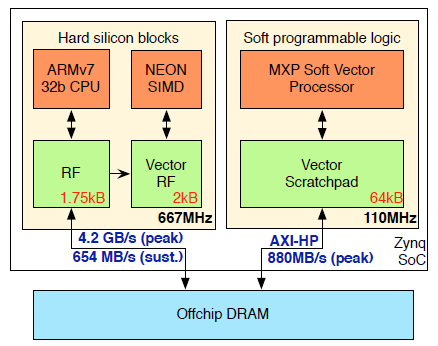
\includegraphics[width=0.67\textwidth]{images/arm-neon-mxp.png}
	\caption{Xilinx Zynq SoC Platform Compute Organization~\cite{kapre2016optimizing}}
	\label{arm-neon-mxp}
\end{figure}


As shown in Figure~\ref{table-arm-neon-mxp}, For byte-level operations, ARMv7 processor is able to provide a peak performance of 0.66 Giga-operations per second (GOPS).
Despite the fact that NEON can perform 8 byte-level operations every clock cycle and able to provide a peak performance of 5.3 GOPS, most compute kernels suffer to take advantage of the performance of NEON engine. 

\begin{figure}
	\centering
	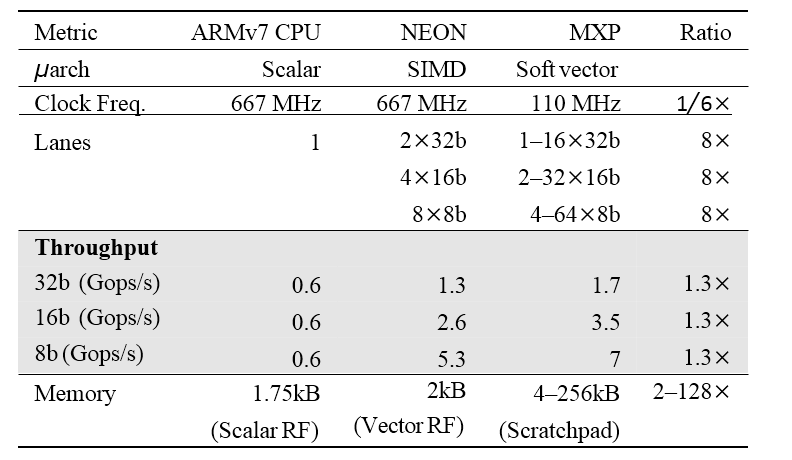
\includegraphics[width=0.67\textwidth]{images/table-arm-neon-mxp.png}
	\caption{Architecture Specifications~\cite{kapre2016optimizing}}
	\label{table-arm-neon-mxp}
\end{figure}



For example, ARMv7 and NEON can provide a performance of only 325 MOPS and 990 MOPS, respectively for quadratic polynomial (as shown in Figure~\ref{quad-poly}). On the other hand, 64-lane MXP soft processor (a carefully designed vector-engine) running at 110 MHz can provide a peak performance of 7 GOPS and while executing quadratic polynomial it can provide a performance of 1.51 GOPS, which is much faster than ARMv7 ($4.75\times$) and NEON ($1.56\times$).





\begin{figure}
	\centering
	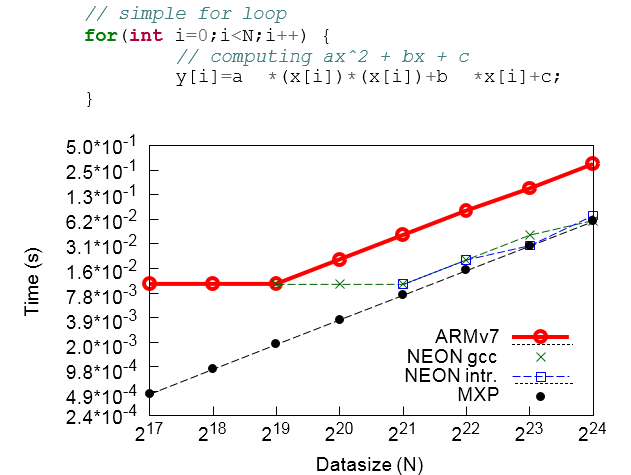
\includegraphics[width=0.9\textwidth]{images/quad-poly.png}
	\caption{Comparing runtime for $a*x^2 + b*x + c$~\cite{kapre2016optimizing}}
	\label{quad-poly}
\end{figure}


In this report, we first analyze compute kernels by extracting data flow graphs and then evaluate the performance of computing platforms such as ARMv7, NEON, Intel processor, and MXP soft vector-engine. The goal is to quatify the gap between peak performance of the platform and achievable performance for a set of compute kernels. 
Major focus of this report is on MXP soft vector-engine which we instantiate on Zynq device available on Zedboard platform.
Apart from using compute kernels to evaluate the performance, we also use a simple image processing application and a complex benchmark (SpMV) to better understand the performance gap.





\section{Contribution}
The main contributions can be summarized as follows:

\begin{itemize}
	\item Setting up Linux and accessing MXP overlay through it so that in future much more attention can be given on building up the MXP application rather than struggling to configure Linux for the MXP overlay.
	\item Comparing the MXP overlay performance against other processors like Intel I3, ARMv7 and NEON hard vector engine for a set of compute kernels.
	\item Accelerating image processing application and a complex benchmark (SpMV) using MXP APIs.
\end{itemize}

\section{Organization}
The remainder of the report is organized as follows:

Chapter 2 gives background information about different computing platforms and most importantly about the MXP vector processor, refer to as an overlay as well. In chapter 3, we describe about the MXP vector processor, it's architecture in detail and the concept of overlapping computation with communication that make it more effective in terms of throughput as compared to other embedded hard vector processors. In chapter 4, we discuss how we configure Linux for MXP on Xilinx ZedBoard so that we can provide OS support for MXP on the Xilinx ZedBoard. In chapter 5, we describe about our experimentation for the performance analysis of MXP vector processor while accelerating compute kernels. In chapter 6, we describe about our experimentation for runtime analysis of image processing application and SpMV computational kernel. We conclude in chapter 7 and discuss future work.








%Field-Programmable Gate Arrays (FPGAs) provides an easier way than Application Specific Integrated Circuits (ASICs) for the implementation of different computing platforms. FPGAs generally yield higher performance and lower power than optimized software running on high-end CPUs. However, designing hardware with FPGAs remains a difficult and time-consuming process. It requires specialized skills and hours-long CAD processing times \cite{1}. The slow place-and-route cycles while accelerating computations using programmable fabric (FPGAs) and non- availability of suitable abstractions prohibits commercial use of such platforms and thus restricting their effective usage to the hardware experts. FPGA virtualization, which is nothing but the use of the overlay architecture such as MXP soft-vector processor, has emerged as an attractive solution by providing fast compilation, run-time management and software-like programmability. These soft processors can extend the capability of embedded hard vector processors because of their improved design productivity and higher-level design abstraction. With the increasing complexity of FPGA platforms, it is being said that the use of overlay architecture will become mainstream \cite{2}. Moreover, the use of Operating system (OS) in a reconfigurable platform helps in managing various hardware tasks, better management of memory and management of the shared resources across the applications. Integrating an overlay architecture with memory subsystem and processor is very important to manage and enable sharing of limited overlay resources. Overlays exhibit features independent from the host FPGA.

\newpage
\chapter{Background}

\section{High Performance Computing}

Accelerated Computing also known as computational acceleration has led to an era of high performance computing (a.k.a HPC). Moore's law has been widely accepted as an industry standard and these industries were highly dependent on Moore's law for better performance and improved efficiency. It was cited by most of the semiconductor manufacturers as they strive to increase computational power. Every year, the transistors that were being added on the silicon area were very fast and consumed less amount of power. But, in recent years, Moore's Law has slowed down by a considerable amount since as the number of the transistor on the chip increases, the frequency stopped scaling. Hence, it became very difficult to extract the performance from a single core processor (sequential CPU). Moreover, single processor ran into memory wall and power wall issues. Thus, adding more CPU cores was a solution from where the multicore processor emerged. However, with multiple CPU cores, it became difficult to gain better performance out of these chips. The challenge was writing the code that can run across multiple cores simultaneously. Moreover, some instructions can't run simultaneously at all. So, the computing world ended up with multicore CPUs that could not accelerate all types of code. This made the designer’s job even harder. Simply adding cores resulted into waste of transistors and raised the cost to manufacture the processor without much benefit. Failure to improve the performance of CPU, without affecting power budgets or using extremely complicated design methods resulted in the industry hitting a brick wall.

“Accelerated Computing has reached a tipping point in the High-Performance Computing. Within a year or two, the majority of the system will be equipped with accelerators”. \cite{2}

Heterogenous computing refers to systems that make use of more than one kind of processors. Performance gain or energy efficiency is achieved in these systems by adding dissimilar coprocessors for handling multiple type of tasks using their specialized computational/processing capabilities. Accelerated computing is a computing model used for accelerating applications in engineering and scientific domains wherein the computations are performed on specialized processors accelerators. It makes use of heterogeneous computing systems for improving the performance of application in which a lot of data is executed in parallel. The basic idea is to execute the code that is suitable for a processor. For example, sequential code with a lot of control instructions and branches would be preferred to run over a CPU since they would provide better performance for this kind of code, whereas computation which is highly parallel with very less branching conditions would be well suited for execution on the accelerator.


\section{FPGA Virtualization for High Performance Computing}

Virtualization of FPGA using the FPGA overlays delivers high performance for application acceleration \cite{3}. With the increasing complexity of FPGA platforms, it is being said that the use of overlay architecture will become mainstream. Overlay architecture can enable widespread use of the FPGAs in accelerated computing. FPGAs make the full utilization and advantage of Moore's Law improvements in semiconductor technology \cite{4}. Reconfigurable platforms consisting of general-purpose processors along with the programmable logic have been introduced by the major FPGA vendors like Xilinx and Altera. FPGAs are used for high speed computations for the data parallel applications. However, it remains difficult to develop an accelerator using Hardware Description Language (HDL). It requires expertise in hardware designing performing implementation and debugging for building hardware. Hardware design, design productivity and long compilation times are few of the barriers that restricts the use of FPGA in general purpose computing.

FPGA virtualization using Overlay architecture offers the advantage of the fast compilation, run-time management and software-like programmability because of their improved design productivity and high-level design abstraction \cite{5}, \cite{6},\cite{7}. Other benefits include better design reuse, application portability across platforms and rapid reconfiguration that is much faster than partial reconfiguration on fine grained FPGAs. Integrating overlays with memory subsystem and processor is important to enable sharing and management of limited overlay resources. Overlays exhibit features independent from the host FPGA. Soft processors can extend the capability of embedded hard vector processors in FPGA like Xilinx Zynq.

In this thesis work, we are going to use an overlay architecture known as MXP soft-processor used for high performance computing in our experiments while analysing the runtime, speedup and throughput obtained. It is a soft vector processor developed by Vectorblox Computing Inc \cite{8} and is classified as Single Instruction, Multiple Data (SIMD) Stream processor. It is provided as an IP core which can be instantiated over the FPGA. It provides the acceleration of the data parallel operations. MXP Vectorblox can be programmed in C/C++ and provides different C/C++ APIs support. This helps to program it easily rather than struggling a lot with Hardware Description Languages like VHDL or Verilog. For using an accelerator over FPGA, the hardware designing flow requires to go through a long design cycle (taking up hours to weeks) whereas on the other hand using MXP, all we need to do is to alter the given software code. MXPs parameterized design helps user to specify the amount of parallelism needed, which can range from 1 to 128. It includes a parallel access local scratchpad memory which holds the data and a high-throughput Direct Memory Access (DMA). MXP can be easily instantiated in the existing Xilinx and Altera development boards, simplifying the development.

In our work we have used Xilinx Zynq 7020 SoC \cite{9} heterogeneous computing platform wherein the MXP soft-processor is instantiated on its programmable logic fabric. Now, we will discuss about the hardware platform which we have used in detail.


\section{Zynq-7000 SOC Board}

Xilinx ZedBoard is a SOC development board which is based on Xilinx Zynq-7000 All Programmable SoC (AP SoC) \cite{10}. ZedBoard is a platform which is partitioned into Processing system (PS) consisting of one or multiple processors along with memory interfaces, bus and peripherals and the Programmable Logic. It provides a way in which even a customized hardware can be instantiated. These two parts are connected via high throughput interconnect to maximize communication bandwidth. ZedBoard features are shown below in table~\ref{zz:123}.

\begin{table}[htbp]
	\centering
	\begin{adjustbox}{width=.6\textwidth}
		\small
	
	\begin{tabular}{rl}
		\toprule
		\multicolumn{1}{l}{\textbf{Feature }} & \textbf{Description} \\
		\midrule
	    \multicolumn{1}{l}{Processor } & Zynq-7000 AP SoC XC7Z020-CLG-484-1 \\
		\midrule
	    \multicolumn{1}{l}{Memory } & 512 MB DDR3 \\
	      & 256 MB Quad-SPI Flash \\
	      & 4.0 GB SD card \\
		\midrule
	    \multicolumn{1}{l}{Communication} & Onboard USB-JTAG Programming \\
	      & USB OTG 2.0 and USB-UART \\
	      & 10/100/1000 Ethernet \\
		\midrule
	    \multicolumn{1}{l}{Expansion Connectors} & Expansion connectors  \\
	      & FMC-LPC connector  \\
	      & Five Pmod compatible header(2x6) \\
	      & Agile Mixed Signalling (AMS) header \\
		\midrule
	    \multicolumn{1}{l}{Clocking } & 33.33 MHz clock source for PS \\
	      & 100 Mhz oscillator for PL  \\
		\midrule
	    \multicolumn{1}{l}{Display } & HDMI output supporting 1080p60 with 16-bit \\
	      & YCbCr \\
	      & 4:2:2 mode color  \\
	      & VGA output (12-bit resolution color) \\
		\midrule
	    \multicolumn{1}{l}{Configuration and Debug} & Onboard USB-JTAG interface \\
	      & Xilinx Platform Cable JTAG connector \\
		\midrule
	    \multicolumn{1}{l}{General Purpose I/O} & Eight user LEDs  \\
	      & Seven push buttons \\
	      & Eight DIP switches \\
		\bottomrule	
	\end{tabular}%
    \end{adjustbox}
  \caption{ZedBoard Features}
  \label{zz:123}%
   \end{table}%



Figure~\ref{zed:blk} represents ZedBoard block diagram \cite{11}. It gives a brief idea about the Zynq xc7z020-clg484 System On Chip Development Board.

\begin{figure}
	\centering
	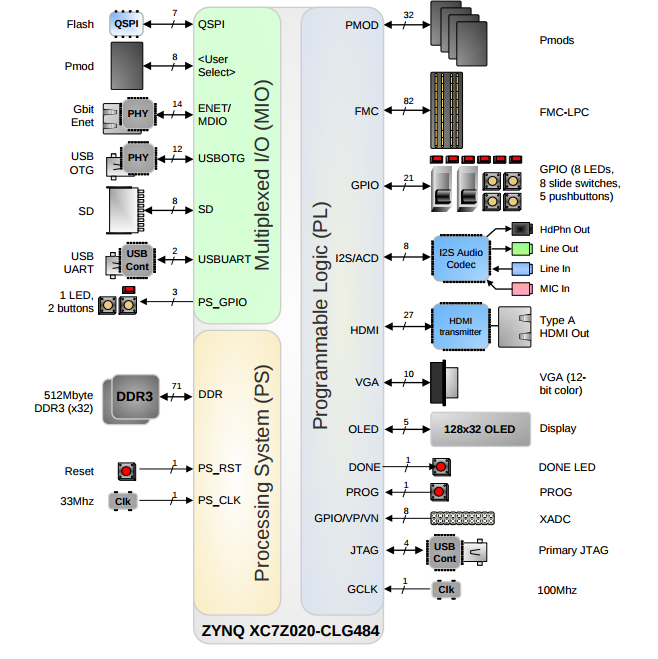
\includegraphics[width=0.9\textwidth]{images/zedboard_block.png}
	\caption{ZedBoard Block Diagram\cite{11}}
	\label{zed:blk}
\end{figure}

FPGA fabric provides the power of reconfigurability along with application specific acceleration while letting the processor execute control intensive tasks. Xilinx Zynq ZedBoard is a development and evaluation board which is based on Zynq-7000 All Programmable SoC architecture. It consists of Zynq Z7020-clg484 of speed grade -1(667 MHz) containing dual core ARM-Cortex A9 based processing system(PS) and PL fabric in one package \cite{12}. The PS consists of a floating-point unit (double precision), DMA controller, 512 MB DDR RAM, commonly used peripherals and external memory interfaces. The components of PS are listed as below:


\begin{itemize}
	\item Two ARM Cortex-A9 cores that are run-time configurable as a single processor.
	\item NEON 128b SIMD coprocessor and VFPv3 per processor.
	\item 512KB L2 cache that is shared between the processors.
	\item 32KB instruction and L1 data caches per processor.
	\item Snoop Control Unit (SCU) and the ACP for cache coherent accesses.
	\item On-Chip Memory (OCM) with capacity of 256KB.
	\item DMA controller with four channels for PS and PL.
	\item DDR controller.
	\end{itemize}

The PL is made up of Artix 7 FPGA fabric \cite{12}. It has 6-input lookup tables (LUTs) and 36kb Block RAMs which can be configured as two 18 Kb blocks. The processor in the system is first booted and PL is configured as a part of boot process or can be configured sometime later in the future. PL can be either reconfigured completely or partially by making use of the partial reconfiguration (PR) feature. The PL configuration data is referred to as bitstream. PL is useful for real-time applications as it has predictable latency. Power can be managed by powering down the PL as it has a different power domain than the PS. The PL has a rich architecture capable of user configuration which are listed below:

\begin{itemize}
\item Configurable logic blocks (CLB) with 6-input lookup table (LUT).
\item DSP48E1 Slices consisting ALU useful for Digital signal processing.
\item 36KB block RAM with capability of dual port.
\item Low jitter clock distribution and low skew.
\item High performance I/Os that can be configured.
\end{itemize}

The ARM based reconfigurable system on ZedBoard makes use of multiple AXI interfaces for communication between the PS and the PL. Each interface provides AXI channels, which helps in efficient data transfer and eliminates performance bottlenecks for memory and I/O. There are three types of AXI interfaces to the fabric mentioned below:

\begin{itemize}
\item AXI GP - Two 32-bit AXI master and two 32-bit AXI slave General purpose (GP ports).
\item AXI HP - Four 32-bit/64-bit configurable, AXI slave High Performance (HP) ports which are buffered along with direct access to DDR and OCM.
\item AXI ACP - One 64-bit AXI Accelerator Coherency Port (ACP) slave interface ensuring access to memory is coherent. AXI ACP - One 64-bit AXI Accelerator Coherency Port (ACP) slave interface.
\end{itemize}

\begin{figure}
	\centering
	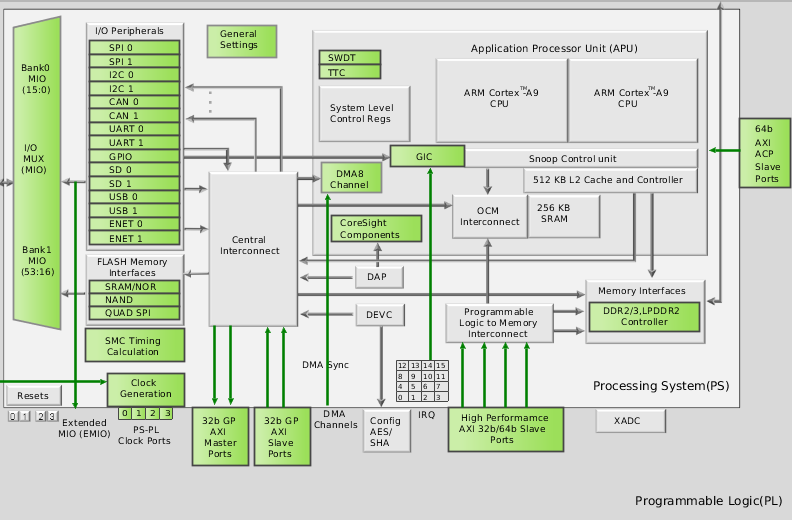
\includegraphics[width=0.9\textwidth]{images/zynqblockdiagram.png}
	\caption{Zynq Block Diagram\cite{12}}
	\label{zynq:blk}
\end{figure}


Figure~\ref{zynq:blk} represents the Zynq block diagram consisting of the Processing System and Programmable Logic(Fabric).

\section{OS Support for Programmable Fabric}
Efficient runtime scheduling of the software and the hardware tasks can be achieved using the Operating System support on the programmable fabric \cite{13}, \cite{14}. It simplifies the programming model. It relieves the user from the responsibility of managing the physical resources like input/output devices, memory and processors. Usage of reconfigurable platforms helps in efficient memory management, coordinating multiple hardware tasks and managing shared resources across the applications \cite{15}. Particularly, the presence of open-source operating system like Linux provides a good control over scheduling of tasks, synchronization, interrupt management etc. Due to overheads introduced, Linux applications will not perform as efficient compared to bare-metal applications, but as they are heavily abstracted from the underlying hardware, it simplifies application development for software developers. Thus, bare metal application requires explicit handling of the resources, synchronization and communication. Xillybus \cite{16} is among one of them that provides the Operating System support on the FPGA.

We came up with the procedure for setting Linux on ZedBoard for MXP applications. Experience gained from booting Linux on ZedBoard \cite{17} and with some hints from the Linux setup for using MXP \cite{18} made it possible to run Linux on ZedBoard for the MXP applications. Detailed description about the MXP architecture is provided in chapter 3 and the procedure for setting Linux on ZedBoard for the MXP will be discussed in chapter 4. This will help in better understanding of the booting process and in future we don’t have to deal with the set-up issues of Linux for the MXP. Furthermore, in the chapter 5, we will calculate the MXP performance against some standards benchmarks. In the chapter 6, we will have a brief discussion about the performance of MXP while dealing with the image processing application.  


\newpage
\chapter{MXP for High Performance Computing}

\section{VectorBlox MXP Matrix Processor}
VectorBlox MXP is a scalable supercomputer on FPGA. It is a SIMD accelerator, available as an IP core. MXP consist of the scratchpad memory which is its local memory and all vector operations are performed directly upon it which maximizes its performance. Unlike traditional processors which have address and data registers, there are no load-stores of vector data in MXP \cite{19}. The architecture of MXP is composed of DMA engine and vector engine. MXP soft-processor provides maximum improved performance because the DMA and vector engine can run at a frequency which is different from the host CPU frequency. DMA engine is used to transfer the data to the local scratchpad. Since MXP implements DMA to access the DDR memory directly, the cache-hierarchy is bypassed. Vector engine is composed of multiple parallel vector lanes, the number of which can be configured from 1 to 256 and 4KB of scratchpad is available for each vector lane. Each lane consists of 32-bit ALU and 4KB of scratchpad memory. The scratchpad and ALU can be divided to perform operations on 16-bits/halfword or 8-bits/byte of data. Thus, the architecture of the MXP soft processor during the byte (8-bits) and half-word (16-bits) level operation provides four and two times the performance respectively as compared to the performance obtained for word level operation. 

\begin{figure}
	\centering
	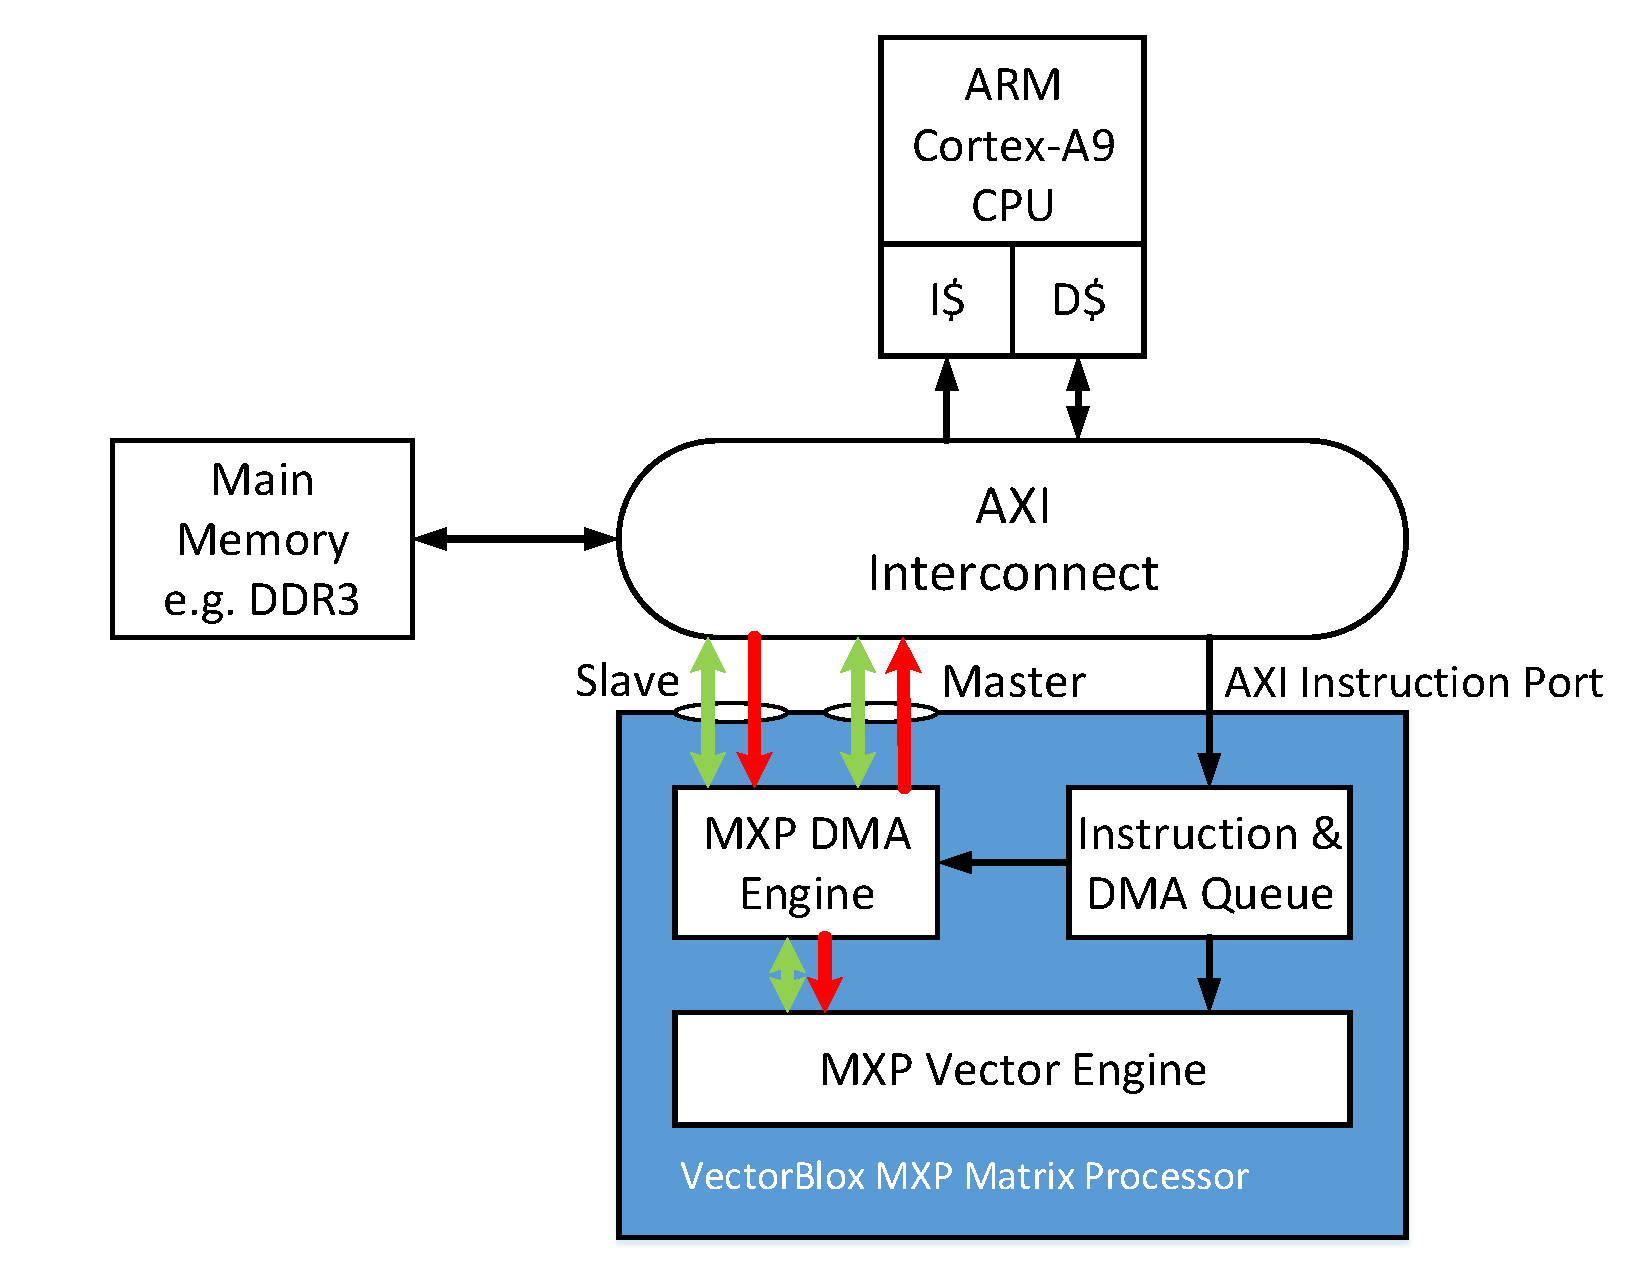
\includegraphics[width=0.9\textwidth]{images/mxp_diagram.pdf}
	\caption{Matrix Processor on ZedBoard\cite{19}}
	\label{zynq:mat}
\end{figure}

MXP vector processor is instantiated onto the programmable logic of the Zynq ZedBoard SoC as shown in Figure~\ref{zynq:mat}. The communication with ARM processor happens via general purpose ports whereas high performance ports are used for communication with the DDR memory. With 64 KB of scratchpad, we can put 32 16-bit lanes/ 16 32-bit lanes / 64 8-bit lanes. The instruction port uses a dedicated AXI slave interface connecting to master GP port on PS. The scratchpad also connects its slave interface to PS through one of the master GP ports. The DMA engine is connected to the DDR memory controller though AXI slave HP ports. Maximum frequency achievable for the 16-lane MXP soft processor is 110 MHz.

VectorBlox MXP can exploit the data parallelism in the computation by organizing the hardware into a tightly coupled array of the compute units that all execute the same instruction in the same cycle.

\subsection{Scratchpad}
MXP do not consist of any data or address registers. It performs all computations using scratchpad. This is used to maximize the performance as it prevents in performing the fetch and load. It does not require additional memory to hold the values.

The primary mechanism to transfer the data to the scratchpad is using the DMA (Direct Memory Access). Host processor can access the elements present in the scratchpad directly.

\subsection{Other Processor State}
MXP soft-processor consist of 32 bits control registers. First 16 registers are used for only hardware. Second group of control registers are software defined.

\subsection{Overlapping Communication with Computation}
Overlapping of the Communication with Computation is necessary to obtain maximum performance. Large set of data are processed usually by decomposing the computation into smaller blocks which further depends on the scratchpad size, and processing chunk of block simultaneously when other block is being transferred. Hence, the time required for transferring the data to the local scratchpad is hidden during the actual computation.   

\begin{figure}
	\centering
	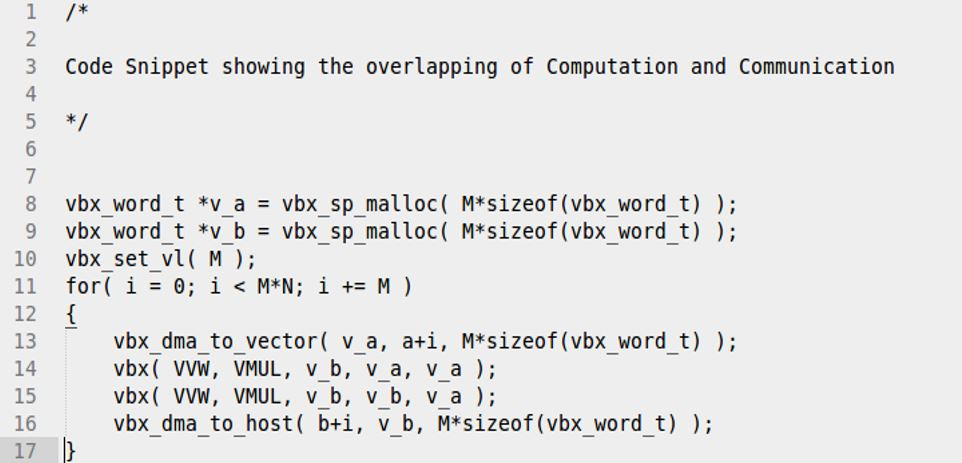
\includegraphics[width=0.9\textwidth]{images/c1.png}
	\caption{Overlapping of the Computation and Communication}
	\label{c1:mat}
\end{figure}

For example, consider the code in figure~\ref{c1:mat}, which calculates the cube of a and puts the result in variable b. It utilizes small blocks having size of M and the dataset being used is having a size of M*N.

For improved performance and efficiency, the code can be rewritten in such a way that the computation and communication can be overlapped. Double buffering is one of the methods through which you can achieve the overlapping of computation and communication. In this technique, one buffer holds the current processing data while the other buffer job is to transfer data in and out of the local scratchpad.

\begin{figure}
	\centering
	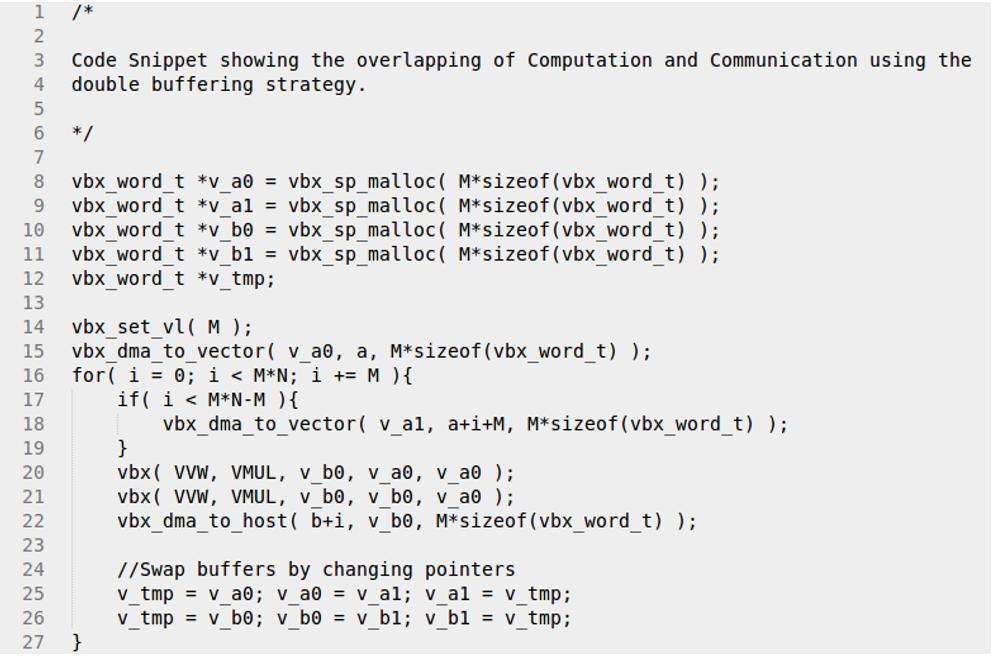
\includegraphics[width=0.9\textwidth]{images/c2.png}
	\caption{Overlapping Computation with Communication}
	\label{c2:mat}
\end{figure}

Consider the code in figure~\ref{c2:mat} which shows the overlapping of the communication and computation.
The same concept is used in measuring the performance for huge set of input data samples in chapter 5.


\section{Programming Model}
A basic program for MXP can be written by following the procedure below:

\begin{enumerate}

	\item Allocate the vectors in local scratchpad.

	\item DMA transfer from DDR to the local scratchpad.

	\item Set the vector length register. It indicates the number of vector elements on which the vector operations are to be performed.

	\item Perform vector operations and obtain result.

	\item Move data from the scratchpad to DDR. DMA transfer of result from local scratchpad to the DDR.

\end{enumerate}

\begin{figure}
	\centering
	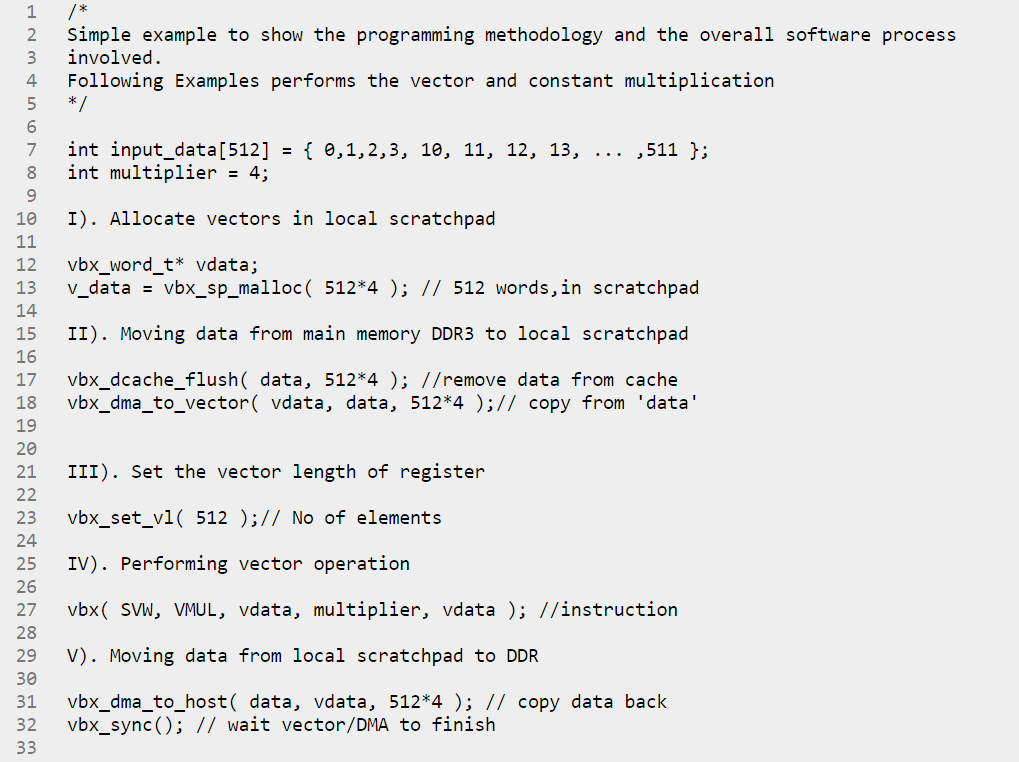
\includegraphics[width=1.2\textwidth]{images/MXPProcess.png}
	\caption{Overall Software Process followed by MXP}
	\label{c3:mat}
\end{figure}



A sample example to explain the methodology is shown in Figure~\ref{c3:mat} The details of the programming methodology used can be found at \cite{19}. The figure shows a sample MXP program with the overall software process followed by MXP. The program shown in Figure~\ref{c3:mat} works fine in a bare-metal system. 

%\subsection{What if we want to run any image and audio processing application?}

In the case when we want to run any image and audio processing application, we will need a filesystem through which information in form of bytes from the input file can be extracted without having to manually enter values as in the example above. Also, the results after processing needs to be written to a file in the appropriate file format depending on the input file type. Vectorblox do provide sources for Linux containing necessary device drivers along with prebuilt bitstreams and hardware design file generated through Vivado.

We provide detailed steps for setting up Linux OS to use MXP on the ZedBoard so that it becomes easy for others to develop application and make full use of the system. Chapter 4 consist of the detailed information on how the Linux can be set up to use MXP.


\newpage
\chapter{OS Support for MXP}
\section{Configuring the Linux For MXP on Xilinx ZedBoard}

Vivado Design Suite 2016 along with the SDK option is installed so that cross-compiler which is required for building the Linux kernel sources is already installed. We don't require to install cross-compiler toolchain for ARM now. We plan to use a persistent filesystem rather than ramdisk since ramdisk lose changes made to filesystem when the board is powered off. Xillybus on ZedBoard along with SD card with a persistent root filesystem was made ready. Next step was the need to build FSBL (First Stage Boot Loader), device tree, U-boot, and the Linux kernel for booting up the board along with the required MXP setup. For this we need to clone the following repositories from GitHub.

\begin{enumerate}

	\item MXP repo: \url{https://github.com/VectorBlox/mxp.git}

	\item Linux repo: 	 \url{https://github.com/VectorBlox/linux-xlnx.git}

	\item U-boot repo: \url{https://github.com/Xilinx/u-boot-xlnx.git}

	\item Device-tree repo: \url{https://github.com/Xilinx/device-tree-xlnx.git}

\end{enumerate}

\begin{figure}
	\centering
	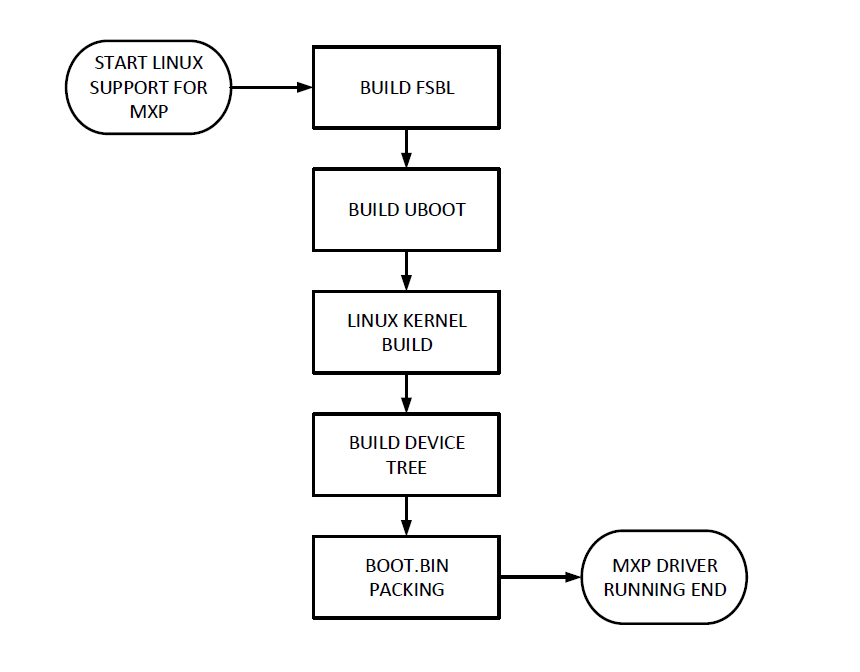
\includegraphics[width=.9\textwidth]{images/bootloader.png}
 
	\caption{Flowchart for Linux setup}
	\label{zed:boot}
\end{figure}



Inside the MXP repository, prebuilt bitstream (named system wrapper.bit to be instantiated on the FPGA) and hardware design file (named system.hdf) have been provided for 8 and 16 vector lanes configuration. We used the one with 16 vector lanes. Steps for setting up Linux on the ZedBoard for MXP are represented using the flowchart shown in figure~\ref{zed:boot} and have been explained in detail later in this chapter.

\section{Building First Stage Bootloader}


Inside the MXP repository, navigate to folder prebuilt\_zedboard\_arm\_viv\_v16 and type commands shown next. Once done rename executable.elf inside mxp\_fsbl to fsbl.elf.


\lstinputlisting[language=c,firstline=96, lastline=101, frame=none,numbers=left,basicstyle=\fontsize{11}{11}\selectfont\ttfamily, backgroundcolor=\color{gainsboro}]{codes.c}

\section{Building U-BOOT}

\begin{enumerate}
	\item Navigate to u-boot repository. We plan to use persistent filesystem rather than ramdisk. Below modifications are necessary in file include/configs/zynq common.h. Find sdboot entry and edit it. This is used to avoid loading ramdisk and make the filesystem persistent.
	
	\lstinputlisting[firstline=1, lastline=14, frame=none,numbers=left,basicstyle=\fontsize{11}{11}\selectfont\ttfamily, backgroundcolor=\color{gainsboro}]{CodeSnippet.txt}
	
	\item Then to compile u-boot give commands as shown below:
		\lstinputlisting[firstline=16, lastline=20, frame=none,numbers=left,basicstyle=\fontsize{11}{11}\selectfont\ttfamily, backgroundcolor=\color{gainsboro}]{CodeSnippet.txt}
		
\end{enumerate}

We renamed u-boot to u-boot.elf and while building Linux kernel we need mkimage utility, so add the tools/ folder to the \$PATH variable.

\section{Linux Kernel Build}

\begin{enumerate}
	\item Navigate to Linux repository and type the following commands.
	
	\lstinputlisting[firstline=22, lastline=23, frame=none,numbers=left,basicstyle=\fontsize{11}{11}\selectfont\ttfamily, backgroundcolor=\color{gainsboro}]{CodeSnippet.txt}
	
	This will generate a .config file.
	
	\item For building the kernel supporting the MXP we need to find out the necessary configuration parameters which needs to be tweaked. To do this, we do reverse engineering. If we look at example source codes provided in the bmark (benchmark) directory of MXP repo, we see the first function to be called in these sample examples is vbx\_test\_init(). For these source codes to run on Linux, this function calls VectorBlox MXP Initialize ("mxp0", "cma"). If we look at the definition of this function, it uses device files \/dev\/mxp0 and \/dev\/cma to do some memory mapping and other initializations. Since these device files are used, there must be corresponding device drivers for them in the Linux source. We surely find files named mxp.c and cma.c in the drivers/char/ directory which are responsible for creating these device files. We then look at the Makefile in drivers/char/ directory and find entries for these files as shown below:
	
	\lstinputlisting[firstline=25, lastline=26, frame=none,numbers=left,basicstyle=\fontsize{11}{11}\selectfont\ttfamily, backgroundcolor=\color{gainsboro}]{CodeSnippet.txt}
	
	Now we have the configuration parameters and hence we edit the .config file generated in step 1 and set these parameters as :
	
	\lstinputlisting[firstline=28, lastline=29, frame=none,numbers=left,basicstyle=\fontsize{11}{11}\selectfont\ttfamily, backgroundcolor=\color{gainsboro}]{CodeSnippet.txt}
	
	\item Compile the kernel and kernel modules:
	\lstinputlisting[firstline=31, lastline=32, frame=none,numbers=left,basicstyle=\fontsize{11}{11}\selectfont\ttfamily, backgroundcolor=\color{gainsboro}]{CodeSnippet.txt}
	
	This will generate compiled kernel uImage in arch/arm/boot/ directory.
	
	\item Insert the SD card with Xillybus setup into the computer where this kernel is compiled and give:
	
		\lstinputlisting[firstline=34, lastline=35, frame=none,numbers=left,basicstyle=\fontsize{11}{11}\selectfont\ttfamily, backgroundcolor=\color{gainsboro}]{CodeSnippet.txt}
		
	This will copy all the kernel modules built in step 4 into the path: IN-
	STALL MOD PATH/lib/modules/\{kernel image name\}/
	
\end{enumerate}

\section{Building Device Tree}

\begin{enumerate}
	\item Inside Linux repo, compile device tree source (dts) to generate device tree blob (dtb).

	\lstinputlisting[firstline=37, lastline=40, frame=none,numbers=left,basicstyle=\fontsize{11}{11}\selectfont\ttfamily, backgroundcolor=\color{gainsboro}]{CodeSnippet.txt}	
	
	To avoid using ramdisk, we replace the contents of bootargs under the chosen node in mxp\_linux.dts as shown:
	
		\lstinputlisting[firstline=42, lastline=46, frame=none,numbers=left,basicstyle=\fontsize{10}{11}\selectfont\ttfamily, backgroundcolor=\color{gainsboro}]{CodeSnippet.txt}
		
	\item Copy folders from drivers/ directory inside MXP repo to the Device tree repo. Navigate to folder prebuilt zedboard\_arm\_viv\_v16 in MXP repo, and enter following commands:
	
			\lstinputlisting[firstline=48, lastline=55, frame=none,numbers=left,basicstyle=\fontsize{11}{11}\selectfont\ttfamily, backgroundcolor=\color{gainsboro}]{CodeSnippet.txt}
			
			\begin{figure}
				\centering
				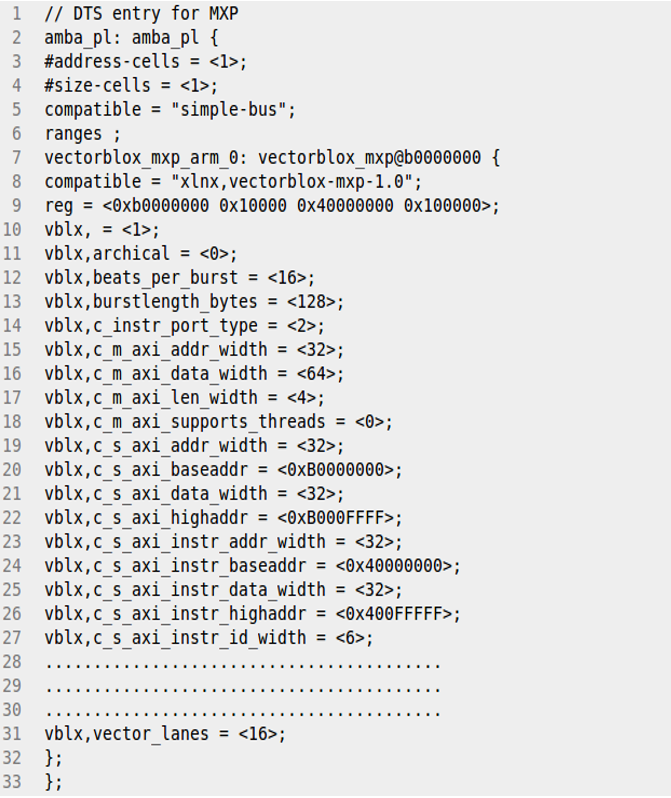
\includegraphics[width=1\textwidth]{images/c4.png}
				\caption{DTS Entry for MXP}
				\label{dts:blk}
			\end{figure}
			
			After this, we see some dts\/dtsi files created inside mxp\_dts folder. We already have the device tree entries corresponding to various peripherals in mxp\_linux.dts file created in step 1. Hence, we are only interested in pl.dtsi files which will contain the device tree node for the MXP soft processor instantiated on programmable logic. Contents in pl.dtsi is as shown in Figure~\ref{dts:blk}.
		
		Given the way in which the device driver file mxp.c parses this device tree
		node, we need to change contents of this file for the correct setup Specifically we need to change compatible string to
	
	\lstinputlisting[firstline=57, lastline=57, frame=none,numbers=left,basicstyle=\fontsize{11}{11}\selectfont\ttfamily, backgroundcolor=\color{gainsboro}]{CodeSnippet.txt}	
	
	Also, the register entry should contain instruction address first. So, node name and reg entry should be changed to
	
		\lstinputlisting[firstline=59, lastline=60, frame=none,numbers=left,basicstyle=\fontsize{11}{11}\selectfont\ttfamily, backgroundcolor=\color{gainsboro}]{CodeSnippet.txt}	
		
		Copy the edited amba\_pl node to the end of mxp\_linux.dts.
		
		\item Finally the device tree is compiled.
	
\lstinputlisting[firstline=62, lastline=62, frame=none,numbers=left,basicstyle=\fontsize{11}{11}\selectfont\ttfamily, backgroundcolor=\color{gainsboro}]{CodeSnippet.txt}			
		
			
\end{enumerate}
	
\section{Packing into BOOT.bin}

Create a file with name, say bootimage.bif. Paste following contents into it

\lstinputlisting[firstline=64, lastline=72, frame=none,numbers=left,basicstyle=\fontsize{11}{11}\selectfont\ttfamily, backgroundcolor=\color{gainsboro}]{CodeSnippet.txt}	

Save the file and generate boot.bin using the command below:

\lstinputlisting[firstline=74, lastline=74, frame=none,numbers=left,basicstyle=\fontsize{11}{11}\selectfont\ttfamily, backgroundcolor=\color{gainsboro}]{CodeSnippet.txt}

Copy files boot.bin, devicetree.dtb and uImage into the FAT partition of sdcard. Plug-in the sdcard and boot ZedBoard. While the kernel is getting loaded we should some message like this

\lstinputlisting[firstline=76, lastline=81, frame=none,numbers=left,basicstyle=\fontsize{11}{11}\selectfont\ttfamily, backgroundcolor=\color{gainsboro}]{CodeSnippet.txt}

This means mxp driver is successfully loaded.

\section{Configuration Parameters of MXP}
We successfully loaded the MXP drivers. The configuration parameters for the MXP setup includes some important parameters named as below:
\begin{enumerate}

	\item vector\_lanes.

	\item core\_freq.

	\item scratchpad\_size.

	\item dma data width in bytes.
 
\end{enumerate}

\lstinputlisting[firstline=83, lastline=87, frame=none,numbers=left,basicstyle=\fontsize{11}{11}\selectfont\ttfamily, backgroundcolor=\color{gainsboro}]{CodeSnippet.txt}


\section{Code for Configuration in Detail}

The configuration details can be found in the below link:

Github Link : \url{https://github.com/AdhikariSaurabh/mxpbenchmarks}


\newpage
\chapter{Performance Analysis of compute kernels}

\section{Benchmarks Evaluation}

The benchmark codes present in the MXP repository provided by VectorBlox gives further idea about the kind of speedup and throughput that can be obtained using MXP soft-vector processor. Scalar time is measured for code running on ARM v7 along with NEON SIMD unit and vector time represents time required when MXP is used for acceleration. We can run the benchmark code and obtain speedup which is the ratio of the scalar time and the vector time. The benchmarks are run on Linux. We need to compile vbxapi library present in MXP repo to use MXP API’s, on Linux.  Once built, this library needs to be linked while compiling the application which we will write on Linux. The results obtained are shown in Table~\ref{t11:tab}.

\begin{table}[htbp]
	\centering
	\begin{adjustbox}{width=1\textwidth}
		\small		
	
	\begin{tabular}{llll}
		\toprule
		\textbf{Benchmark} & \textbf{Scalar time (sec)} & \textbf{Vector time (sec)} & \textbf{Speedup = (Scalar time / Vector time)} \\
		\midrule
			vbw\_mtx\_median\_t & 124e-3 & 5.012e-6 & 24.75 \\
			vbw\_mtx\_sobel & 197.4e-3 & 24.9e-3 & 7.911 \\
			vbw\_vec\_fir\_t & 847e-6 & 58.5e-6 & 14.49 \\
			vbw\_mtx\_fir\_t & 10.62e-3 & 1.75e-3 & 6.057 \\
			vbw\_mtx\_mm\_t & 276e-6 & 18.65e-6 & 14.75 \\
		\bottomrule
	\end{tabular}%
\end{adjustbox}%
\caption{Speedup for the benchmarks on Linux}
\label{t11:tab}%
\end{table}%
%\begin{figure}
%\centering
%\begin{tikzpicture}
%\begin{axis}[
%width  = 0.8*\textwidth,
%height = 8cm,
%%major x tick style = transparent,
%x tick label style={rotate=45, anchor=east, align=right,text width=4cm},
%bar width=8pt,
%ymajorgrids = true,
%ylabel = {Time in $msec$},
%symbolic x coords={vbw\_mtx\_median\_t,vbw\_mtx\_sobel,vbw\_vec\_fir\_t,vbw\_mtx\_fir\_t,vbw\_mtx\_mm\_t},
%xtick = data,
%nodes near coords,
%ybar,
%every node near coord/.append style={rotate=90, anchor=west, font=\scriptsize, xshift=0.25cm},
%scaled y ticks = false,
%enlarge y limits={upper,value=0.2},
%%enlarge x limits=0.25,
%ybar=2*\pgflinewidth,
%legend cell align=left,
%legend style={
%	at={(.5,-0.5)},
%	anchor=north,
%	legend columns=-1
%	column sep=0.5ex
%}
%]
%\addplot[draw=black,fill=blue]
%coordinates {(vbw\_mtx\_median\_t, 124) (vbw\_mtx\_sobel,197.4) (vbw\_vec\_fir\_t,0.847) (vbw\_mtx\_fir\_t,10.62) (vbw\_mtx\_mm\_t,0.276)};
%
%\addplot[draw=black,fill=red, every node near coord/.append style={xshift=-0.25cm}]
%coordinates {(vbw\_mtx\_median\_t, 0.005012) (vbw\_mtx\_sobel,24.9) (vbw\_vec\_fir\_t,0.0585) (vbw\_mtx\_fir\_t,1.75) (vbw\_mtx\_mm\_t,0.01865)};
%
%\addplot[draw=black,fill=yellow,every node near coord/.append style={xshift=-0.55cm}]
%coordinates {(vbw\_mtx\_median\_t,24.75) (vbw\_mtx\_sobel,7.911) (vbw\_vec\_fir\_t,14.49) (vbw\_mtx\_fir\_t,6.057) (vbw\_mtx\_mm\_t,14.75)};
%
%%nodes near coords=\raisebox{1.7cm}{\pgfmathprintnumber\pgfplotspointmeta}
%
%\legend{Scalar time(msec),Vector time(msec), Speedup=(Scalar time / Vector time)}
%\end{axis}
%\end{tikzpicture}
%\caption{Speedup for different benchmarks}
%\label{g1:g1}
%\end{figure}


\pgfplotsset{
	axis background/.style={fill=none},
	tick style=black,
	tick label style=black,
	grid=both,
	xtick pos=left,
	ytick pos=left,
	tick style={
		major grid style={style=white,line width=1pt},minor grid style=white,
		tick align=outside,
	},
	minor tick num=4,
}

\begin{figure*}[!t]
	\centering
	\pgfplotstableread{
		0  124		0.0050    24.75		   
		1  197.4    24.9      7.911	
		2  0.847    0.058     14.49	 
		3  10.62    1.75      6.057    
		4  0.276  	0.0186    14.75    
	}\dataset
	\begin{tikzpicture}
	\centering
	\begin{axis}[ybar=0pt,
	%enlarge x limits=0.05,
	width=25cm,
	x = 1.8cm,
	height=8cm,
	ymin=0,
	ymax=240,        
	ylabel={Time in $msec$},
	grid style={dotted,gray},
	ymajorgrids=true,
	nodes near coords,    
	xtick=data,
	bar width = 0.15,
	xticklabels = {
		\strut vbw\_mtx\_median\_t,
		\strut vbw\_mtx\_sobel,
		\strut vbw\_vec\_fir\_t,
		\strut vbw\_mtx\_fir\_t,
		\strut vbw\_mtx\_mm\_t                                  
	},
	x tick label style={rotate=45, anchor=north east, inner sep=0mm},
	major x tick style = {opacity=0},
	minor x tick num = 1,
	minor tick length=1ex,
	every node near coord/.append style={
		anchor=west,
		rotate=90,
		font=\tiny
	},
	]
	\addplot[draw=black,fill=blue!90, draw opacity=1] table[x index=0,y index=1] \dataset;\label{Scalar time(msec)} %ano de 2013-2014
	\addplot[draw=black,fill=green!90, draw opacity=1] table[x index=0,y index=2] \dataset;\label{Vector time(msec)} %ano de 2012-2013
	\addplot[draw=black,fill=red!90, draw opacity=1] table[x index=0,y index=3] \dataset;\label{Speedup=(Scalar time / Vector time)} %ano de 2012-2013
	\end{axis}
	\node [draw,fill=white] at (rel axis cs: 0.55,-0.50) {\shortstack[l]{
			\ref{Scalar time(msec)} Scalar time(msec) \ref{Vector time(msec)}  Vector time(msec) \ref{Speedup=(Scalar time / Vector time)} Speedup=(Scalar time / Vector time)}};
	
	\end{tikzpicture}
	\caption{Speedup for different benchmarks}
	\label{speedupofnormalbenchmarks}
	
\end{figure*}






The graph showing the speedup of different benchmarks are shown in the Figure~\ref{speedupofnormalbenchmarks}




\section{Accelerating Compute Kernels}
We have taken into consideration a benchmark set shown in the table 5.2 consisting of various compute kernels. These compute kernels are considered from the paperwork \cite{20},\cite{21},\cite{22},\cite{23}.These are quite good benchmarks that can be used to analyze the performance of the MXP soft processor against other embedded processors such as ARM v7, NEON SIMD unit and INTEL i3. We took the throughput as one of the main performance measures and compared the results for various compute kernels.

\begin{table}[htbp]
	\centering
	\begin{adjustbox}{width=.9\textwidth}
		\small
	\begin{tabular}{llllllll}
		\toprule
		\textbf{No} & \textbf{Benchmark Name} & \textbf{Description} & \textbf{Add} & \textbf{Sub} & \textbf{Mul} & \textbf{OR} & \textbf{Operations} \\
		\midrule
		1     & poly  & degree-2 polynomial & 2     &       & 3     &       & 5 \\
		2     & poly  & Degree-3 polynomial & 3     &       & 6     &       & 9 \\
		\midrule
		3     & chebyshev & filter & 1     & 1     & 5     &       & 7 \\
		4     & mibench & filter & 8     &       & 7     &       & 15 \\
		5     & sgfilter & filter & 5     & 4     & 9     &       & 18 \\
		6     & qspline & filter & 4     &       & 23    &       & 27 \\
		\midrule
		7     & fft   & kernel & 3     & 3     & 4     &       & 10 \\
		8     & kmeans & kernel & 7     & 8     & 8     &       & 23 \\
		9     & mm    & kernel & 7     &       & 8     &       & 15 \\
		10    & spmv  & kernel & 6     &       & 8     &       & 14 \\
		11    & stencil & kernel & 10    & 2     & 2     &       & 14 \\
		12    & mri   & kernel & 4     &       & 5     & 1     & 10 \\
		\bottomrule
	\end{tabular}%
\end{adjustbox}%
    \caption{Benchmarks Characteristics}
	\label{b1:g1}%
\end{table}%


The Table~\ref{b1:g1} demonstrates the characteristics of the benchmarks. Total number of the operations which are used to obtain the corresponding DAG (Directed Acyclic Graph) expression for compute kernels and corresponding Add, Sub, Mul and OR operations required are shown in table 5.2. 


Table~\ref{dag:dag} demonstrates the kernel benchmarks along with the DAG expression corresponding to it. We mapped the kernel benchmarks on the MXP soft processor and obtained the corresponding throughput as it's one of the performance criterion that differentiates MXP from the other embedded hard processors.

\begin{table}
	\centering
	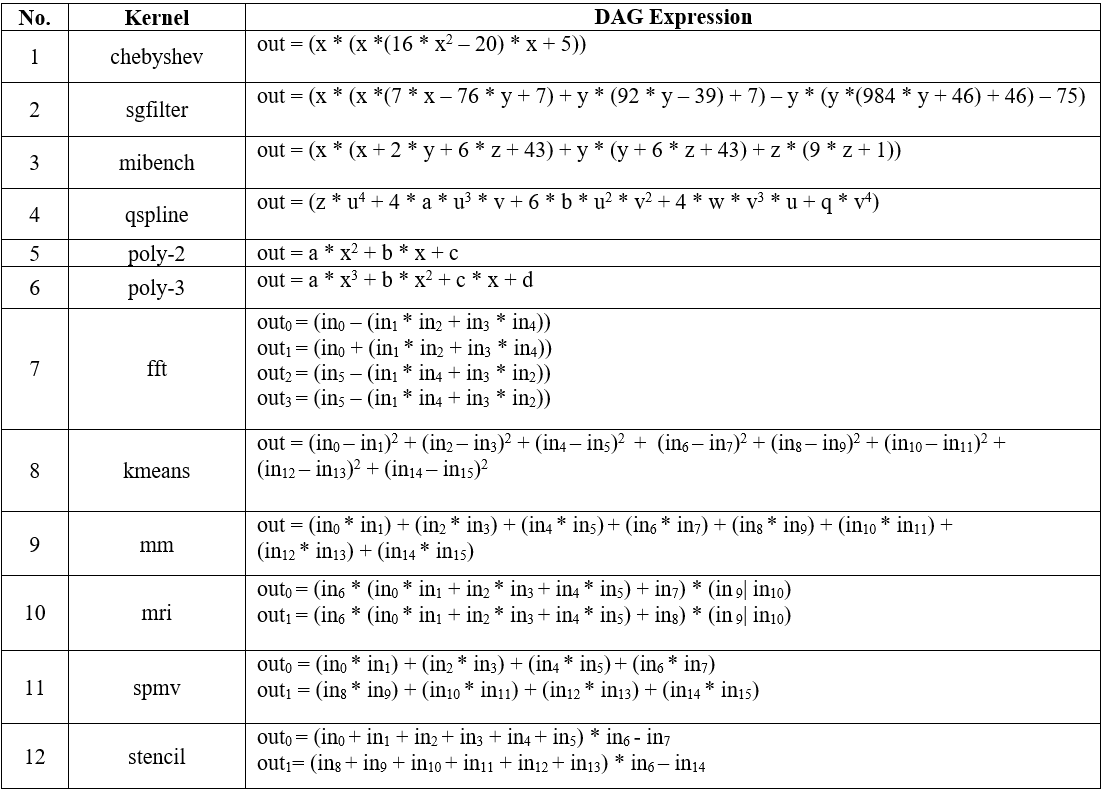
\includegraphics[width=1\textwidth]{images/dag.png}
	\caption{Kernel Benchmarks}
	\label{dag:dag}
\end{table}

\section{Experimentation and Results}

In our work, Xilinx ZedBoard is being used for experimentation and result analysis. We used the gcc for generating the ARM binaries and running the code for the NEON SIMD at the highest optimization level. We used -mfloat-abi=hard -mfpu=neon for running the code on the MXP soft-vector processor.

\subsection{Runtime Comparison}
We compared the runtime for the poly benchmarks (degree-2 and degree-3 polynomial) for huge number of input samples. We observed that MXP outperforms NEON SIMD unit and ARM v7 as it parallelizes the computation and communication. MXP has very high speedups due to the superior double-buffered memory transfer optimization [3.1.3]. The Table~\ref{x:20} and Table~\ref{y:21} represents the runtime in milliseconds for different number of input samples for the poly-2 (quadratic) and poly-3 (cubic) benchmarks respectively. We also plotted a graph between Time in Milliseconds Vs Datasize which shows that the time taken by the MXP soft-vector processor for processing the input samples is very less and provides high speedups. Figure~\ref{dag:q} and Figure~\ref{dag:c} shows the observed runtime for the poly (degree-2 and degree-3) benchmarks. This clearly infers that the MXP soft-vector processor takes less runtime as compared to ARM v7 and Neon while we keep on increasing the number of the input samples. MXP has very high speedups due to the superior double-buffered memory transfer optimization [3.1.3].

\begin{table}[htbp]
	\centering
		\begin{adjustbox}{width=.9\textwidth}
		\small
	\begin{tabular}{lllll}
		\toprule
		\textbf{No of Samples} & \textbf{MXP (ms)} & \textbf{ARMv7 CPU (ms)} & \textbf{INTEL i3 (ms)} & \textbf{NEON(auto vector) (ms)} \\
		\midrule
		$2^{17}$ & 0.4239 & 10 & 0.127 & 0 \\
		$2^{18}$ & 0.884 & 10 & 0.262 & 0 \\
		$2^{19}$ & 1.88 & 10 & 0.654 & 10 \\
		$2^{20}$ & 3.465 & 20 & 1.057 & 10 \\
		$2^{21}$ & 6.949 & 40 & 4.951 & 10 \\
		$2^{22}$ & 13.86 & 70 & 7.962 & 20 \\
		$2^{23}$ & 27.72 & 130 & 9.447 & 40 \\
		$2^{24}$ & 55.46 & 250 & 17.275 & 80 \\
		\bottomrule
	\end{tabular}%
    \end{adjustbox}%
   \caption{Poly-2 Benchmark Runtime in $ms$ for 8-bit data}
	\label{x:20}%
\end{table}%

\begin{table}[htbp]
	\centering
	\begin{adjustbox}{width=.9\textwidth}
		\small
	\begin{tabular}{lllll}
		\toprule
		\textbf{No of Samples} & \textbf{MXP (ms)} & \textbf{ARMv7 CPU (ms)} & \textbf{INTEL i3 (ms)} & \textbf{NEON(auto vector) (ms)} \\
		\midrule
		$2^{17}$ & 0.534 & 10 & 0.127 & 0 \\
		$2^{18}$ & 1.032 & 10 & 0.262 & 0 \\
		$2^{19}$ & 2.064 & 10 & 0.654 & 10 \\
		$2^{20}$ & 4.166 & 30 & 1.057 & 10 \\
		$2^{21}$ & 8.294 & 40 & 4.951 & 20 \\
		$2^{22}$ & 16.50 & 80 & 7.962 & 40 \\
		$2^{23}$ & 33.01 & 160 & 9.447 & 50 \\
		$2^{24}$ & 65.97 & 330 & 17.275 & 80 \\
		
		\bottomrule
	\end{tabular}%
     \end{adjustbox}%
      \caption{Poly-3 Benchmark Runtime in $ms$ for 8-bit data}
	\label{y:21}%
\end{table}%



%% \hfill
%	 \begin{figure}[!b]
%	 \centering 
%	 \begin{tikzpicture}[scale = 1.1]
%	 \begin{semilogyaxis}[
%		xlabel=Datasize$(N)$,
%		ylabel=Time $(ms)$,
%	 % 	scaled ticks=base 10:-5,
%	 xtick pos=left,
%	 ytick pos=left,
%	 ymax = 600,
%	 xmax = 16777216,
%	 yticklabels={1,10,100,1000},
%	 %	symbolic y coords={0.4239,0.847,1.67,3.33,6.69,13.33,26.63,54.41,70,150,290,560},
%	 %  symbolic y coords = {-1,-0.698,-0.522,-0.397,-0.301,-0.221,-0.154,-0.0969,-0.0457,0.0,0.3010,0.4771,0.6021,0.6990,0.7782,0.8450,0.9030,0.9542,1.0,1.3010,1.4771,1.6021,1.6990,1.7782,1.8450,1.9030,1.9542,2.0,2.3010,2.4771,2.6021,2.6990,2.7782,2.8452,2.9030,2.9542,3.0},
%	 %    ytick=data, 
%	 %    yticklabels={0.1,0.2,0.3,0.4,0.5,0.6,0.7,0.8,0.9,1,2,3,4,5,6,7,8,9,10,20,30,40,50,60,70,80,90,100,200,300,400,500,600,700,800,900,1000},
%	 symbolic x coords={131072,262144,524288,1048576,2097152,4194304,8388608,16777216},
%	 enlargelimits=true,
%	 xtick=data,
%	 xticklabels={$2^{17}$,$2^{18}$,$2^{19}$,$2^{20}$,$2^{21}$,$2^{22}$,$2^{23}$,$2^{24}$},
%	 width = 10cm,
%	 xmode = normal,
%	 legend pos=north west,
%	 legend style={draw=none}
%	 ] 
	 
	 
	 % \hfill
	 \begin{figure}[!b]
	 \centering 
	 \begin{tikzpicture}[scale = .8]
	 \begin{semilogyaxis}[
    xlabel=Datasize$(N)$,
	ylabel=Time $(ms)$,
	 % 	scaled ticks=base 10:-5,
	 xtick pos=left,
	 ytick pos=left,
	 ymax = 1000,
	 xmax = 16777216,
	 %	 ymode=log,log ticks with fixed point,
	 %	grid=major,
	 %   symbolic y coords={0.4239, 0.847, 1.67, 3.33, 6.69, 13.33,26.63,54.41},
	 %   ytick={data},
	 symbolic x coords={131072,262144,524288,1048576,2097152,4194304,8388608,16777216},
	 xtick=data,
	 xticklabels={$2^{17}$,$2^{18}$,$2^{19}$,$2^{20}$,$2^{21}$,$2^{22}$,$2^{23}$,$2^{24}$},
	 %	symbolic y coords={0.4239,0.847,1.67,3.33,6.69,13.33,26.63,54.41,70,150,290,560},
	 width = 10cm,
	 xmode = normal,
	 legend pos=north west,
	 legend style={draw=none}
	 ]    
   
	\addplot plot coordinates {
	    (131072,     0.4239)
		(262144,     0.884)
		(524288,    1.88)
		(1048576,    3.465)
		(2097152,    6.949)
		(4194304,    13.86)
		(8388608,   27.72)
		(16777216,   55.46)
		};

%	\addplot plot coordinates {
%	(131072,     0.628)
%	(262144,     1.432)
%	(524288,    2.71)
%	(1048576,    5.266)
%	(2097152,   10.695)
%	(4194304,   21.55)
%	(8388608,   43.143)
%	(16777216,   95.41)
%	
%	};      
	\addplot plot coordinates {
	(131072,     10)
	(262144,     10)
	(524288,    10)
	(1048576,    20)
	(2097152,    40)
	(4194304,    70)
	(8388608,   130)
	(16777216,   250)
	
	};   
   
   	\addplot plot coordinates {
    	(131072,     0)
    	(262144,     0)
    	(524288,    10)
    	(1048576,    10)
    	(2097152,    10)
    	(4194304,    20)
    	(8388608,   40)
    	(16777216,   80)
    
    };   

%	\legend{MXP(Byte)\\Intel i3(Byte)\\ARMv7(Byte)\\Neon(Byte)\\} 
    \legend{MXP(Byte)\\ARMv7(Byte)\\Neon(Byte)\\} 
	\end{semilogyaxis}
	\end{tikzpicture} 
	\label{throughput} 
 \hspace{2.0cm}       $f(samples,time) = a * x ^ 2 + b* x + c$
\caption{Comparing Runtime for \textit{Poly-2} benchmark.} 
\label{dag:q}

\end{figure}

	 % \hfill
	 \begin{figure}[!b]
	 	\centering 
	 	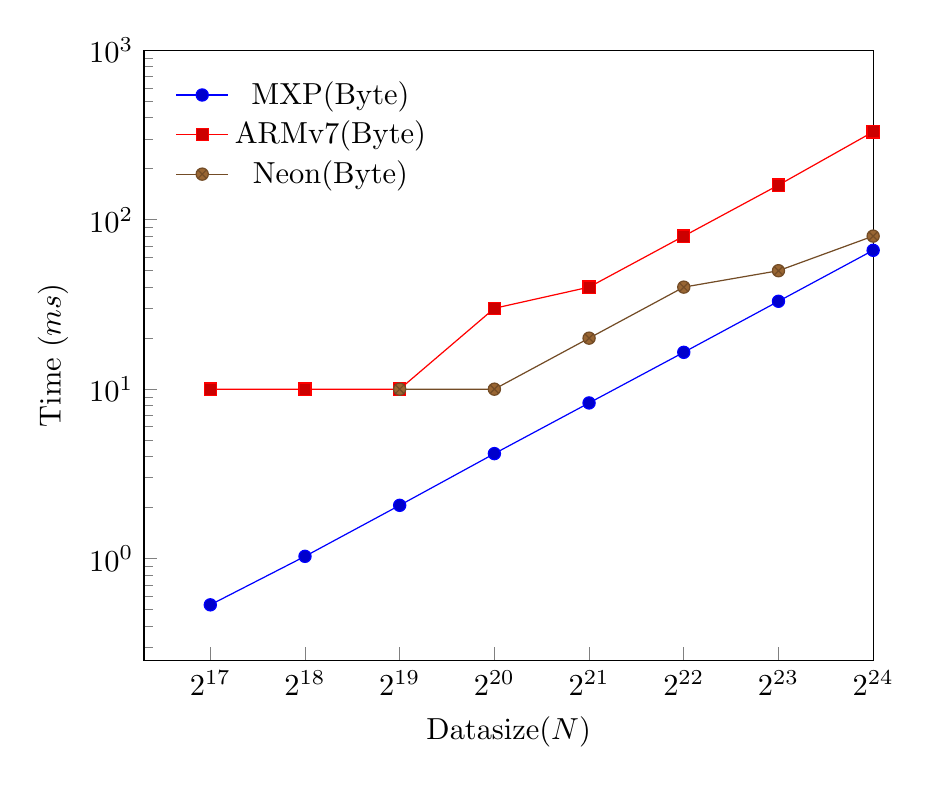
\begin{tikzpicture}[scale = 1.1]
	 	\begin{semilogyaxis}[
	 	xlabel=Datasize$(N)$,
	 	ylabel=Time $(ms)$,
	 	% 	scaled ticks=base 10:-5,
	 	xtick pos=left,
	 	ytick pos=left,
	 	ymax = 1000,
	 	xmax = 16777216,
	 	%	 ymode=log,log ticks with fixed point,
	 	%	grid=major,
	 	%   symbolic y coords={0.4239, 0.847, 1.67, 3.33, 6.69, 13.33,26.63,54.41},
	 	%   ytick={data},
	 	symbolic x coords={131072,262144,524288,1048576,2097152,4194304,8388608,16777216},
	 	xtick=data,
	 	xticklabels={$2^{17}$,$2^{18}$,$2^{19}$,$2^{20}$,$2^{21}$,$2^{22}$,$2^{23}$,$2^{24}$},
	 	%	symbolic y coords={0.4239,0.847,1.67,3.33,6.69,13.33,26.63,54.41,70,150,290,560},
	 	width = 10cm,
	 	xmode = normal,
	 	legend pos=north west,
	 	legend style={draw=none}
	 	]    
	 	
	   	\addplot plot coordinates {
	   		(131072,     0.534)
	   		(262144,     1.032)
	   		(524288,    2.064)
	   		(1048576,    4.166)
	   		(2097152,    8.294)
	   		(4194304,    16.50)
	   		(8388608,   33.01)
	   		(16777216,  65.97)
	   		
	   	};
%	   	\addplot plot coordinates {
%	   		(131072,     0.71)
%	   		(262144,     3.389)
%	   		(524288,    5.86)
%	   		(1048576,    8.431)
%	   		(2097152,   12.075)
%	   		(4194304,   23.431)
%	   		(8388608,   44.572)
%	   		(16777216,   113.9)
%	   		
%	   	};      
	   	\addplot plot coordinates {
	   		(131072,     10)
	   		(262144,     10)
	   		(524288,    10)
	   		(1048576,    30)
	   		(2097152,    40)
	   		(4194304,    80)
	   		(8388608,   160)
	   		(16777216,  330)
	   		
	   	};   
	   	
	   	\addplot plot coordinates {
	   		(131072,     0)
	   		(262144,     0)
	   		(524288,    10)
	   		(1048576,    10)
	   		(2097152,    20)
	   		(4194304,    40)
	   		(8388608,   50)
	   		(16777216,   80)
	   	};   
	   	
	 
%	 \legend{MXP(Byte)\\Intel i3(Byte)\\ARMv7(Byte)\\Neon(Byte)\\} 
	 \legend{MXP(Byte)\\ARMv7(Byte)\\Neon(Byte)\\} 
	 \end{semilogyaxis}
	 \end{tikzpicture} 
	 \label{throughput} 
	}
\hspace{3.5cm}     $f(samples,time) = a * x ^ 3 + b* x ^ 2 + c *x + d$
\caption{Comparing Runtime for \textit{Poly-3} benchmark.} 
\label{dag:c}
	
\end{figure}

\pgfplotsset{
	axis background/.style={fill=none},
	tick style=black,
	tick label style=black,
	grid=both,
	xtick pos=left,
	ytick pos=left,
	tick style={
		major grid style={style=white,line width=1pt},minor grid style=white,
		tick align=outside,
	},
	minor tick num=4,
}

\begin{figure*}[!t]
\centering
\pgfplotstableread{
	0  0.33		0.93	1.5		2.85   
	1  0.4      1.8     2.28	4.74
	2  0.28     0.5     0.75	1.9 
	3  0.35    	0.9     1.14    3.43
	4  0.16    	0.25    0.38    1.77
	5  0.28    	0.43    0.57    2.35
}\dataset
\begin{tikzpicture}
\centering
\begin{axis}[ybar=0pt,
%enlarge x limits=0.05,
width=25cm,
x = 1.8cm,
height=8cm,
ymin=0,
ymax=8,        
ylabel={Throughput in GOPS},
grid style={dotted,gray},
ymajorgrids=true,
nodes near coords,    
xtick=data,
bar width = 0.15,
xticklabels = {
	\strut quad-byte,
	\strut cubic-byte,
	\strut quad-half,
	\strut cubic-half,
	\strut quad-word,
	\strut cubic-word,	                                  
},
x tick label style={rotate=45, anchor=north east, inner sep=0mm},
major x tick style = {opacity=0},
minor x tick num = 1,
minor tick length=1ex,
every node near coord/.append style={
        anchor=west,
        rotate=90,
        font=\tiny
},
]
\addplot[draw=black,fill=blue!90, draw opacity=1] table[x index=0,y index=1] \dataset;\label{ARM} %ano de 2013-2014
\addplot[draw=black,fill=green!90, draw opacity=1] table[x index=0,y index=2] \dataset;\label{NEON} %ano de 2012-2013
\addplot[draw=black,fill=red!90, draw opacity=1] table[x index=0,y index=3] \dataset;\label{MXP} %ano de 2012-2013
\addplot[draw=black,fill=black!90, draw opacity=1] table[x index=0,y index=4] \dataset;\label{Intel-i3} %ano de 2012-2013
\end{axis}
	\node [draw,fill=white] at (rel axis cs: 0.55,0.8) {\shortstack[l]{
			\ref{ARM} ARM \ref{NEON} NEON \ref{MXP} MXP \ref{Intel-i3} Intel-i3}};

\end{tikzpicture}
\caption{The performance comparisons of different architectures for quad and cubic}
\label{throughput}

\end{figure*}



\subsection{Benchmarks Performance Analysis}
In this section, we are going to compare the MXP soft-vector processor with other embedded hard processor such as ARM v7, NEON SIMD unit and INTEL i3. The main criterion of the comparison would be the throughput expressed in terms of Gops/sec.

\subsubsection{Throughput Analysis for poly benchmark}

The compute kernels for the first part of performance comparison work which we took were polynomial with degree-2 (quadratic) and degree-3 (cubic).
We observed that for these benchmarks, MXP has very high throughput when it is operating at the byte(8-bits) level. MXP has very high speedups due to the superior double-buffered memory transfer optimization [3.1.3]. Architecture specification and the corresponding performance in terms of throughput for the poly (degree-2 and degree-3) benchmarks are mentioned in table~\ref{poly:c}.  Figure~\ref{throughput_quad_cubic} demonstrates the average throughput (Gops/sec) obtained while operating on the byte, halfword and word level.

\begin{table}[htbp]
	\centering
	\begin{adjustbox}{width=1\textwidth}
		\small
		\begin{tabular}{llllll}
			\toprule
			\textbf{Metrics} &   & \textbf{ARMv7 CPU} & \textbf{NEON (auto vector)} & \textbf{MXP} & \textbf{INTEL i3} \\
			\midrule
			\textbf{arch} &   & Scalar & SIMD unit & Vector & Scalar \\
			\textbf{clock} &   & $667 X 10^{6}Hz$ & $667 X 10^{6}Hz$ & $110 X 10^{6}Hz$ & $2 X 10^{9}Hz$ \\
			\textbf{no of lanes} &   & 1 & 2 x 32b & 1-16 x 32b & 1 \\
			&   &   & 4 x 16b & 2-32 x 16b &  \\
			&   &   & 8 x 8b & 4-64 x 8b &  \\
			\midrule
			 \textbf{Throughput} & \textbf{Benchmark} &   &   &   &  \\
			\midrule
			 32b(Gops/sec)/ Word   & Quadratic- Poly Deg 2  & 0.1608  & 0.2500 & 0.3782 & 1.77 \\
			 16b(Gops/sec)/Halfword &   & 0.2819 & 0.4988 & 0.758 & 1.914\\
			 8b(Gops/sec)/Byte &   & 0.33656 & 0.9341 & 1.513 & 2.85 \\
			   &   &   &   &   &  \\
			\midrule
			 \textbf{Throughput} & \textbf{Benchmark} &   &   &   &  \\
			\midrule
			 32b(Gops/sec)/ Word   & Cubic- Poly Deg 3    & 0.2886 & 0.4311 & 0.571 & 2.35 \\
			 16b(Gops/sec)/Halfword &   & 0.356 & 0.893 & 1.144 & 3.43 \\
			 8b(Gops/sec)/Byte &   & 0.40054 & 1.7816 & 2.287 & 4.74 \\
			   &   &   &   &   &  \\
			\bottomrule
		\end{tabular}%
	\end{adjustbox}%
	\caption{Throughput(Gops/sec) Analysis for Poly Benchmarks}
	\label{poly:c}%
\end{table}%

%%\begin{figure}
%	\centering
%	\begin{tikzpicture}
%	\begin{axis}[
% 	width  = 0.85*\textwidth,
%	height = 8cm,
%	major x tick style = transparent,
%	bar width=10pt,
%	ymajorgrids = true,
%	ylabel = {Throughput in $Gops/sec$},
%	xlabel = {Poly Benchmarks},
%	symbolic x coords={Quadratic Poly-2,Cubic Poly-3},
%	xtick = data,
%	nodes near coords,
%	ybar,
%	every node near coord/.append style={rotate=90, anchor=west, font=\scriptsize,xshift=0.5cm},
%	scaled y ticks = false,
%	enlarge y limits={upper,value=0.2},
%	enlarge x limits=0.25,
%	ybar=2*\pgflinewidth,
%	legend cell align=left,
%	legend style={
%	at={(.5,-0.2)},
%	anchor=north,
%	legend columns=-1
%	column sep=0.5ex
%}
%	]
%	\addplot[draw=black,fill=blue]
%	coordinates {(Quadratic Poly-2, 1.5130) (Cubic Poly-3,2.287)};
%	
%	\addplot[draw=black,fill=orange,every node near coord/.append style={xshift=-0.25cm}]
%	coordinates {(Quadratic Poly-2,2.85) (Cubic Poly-3,4.74)};
%	
%	\addplot[draw=black,fill=yellow,every node near coord/.append style={xshift=-0.70cm}]
%	coordinates {(Quadratic Poly-2,0.336) (Cubic Poly-3,0.40)};
%	
%	\addplot[draw=black,fill=red,every node near coord/.append style={xshift=-1.10cm}]
%	coordinates {(Quadratic Poly-2,0.9341) (Cubic Poly-3,1.732)};
%	
%	\legend{MXP,Intel i3,ARM v7,NEON}
%	\end{axis}
%	\end{tikzpicture}
%	\caption{Byte(8-bits) level throughput(Gops/sec) for polynomial benchmarks }
%	\label{poly:1}
%\end{figure}
%\begin{figure}
	\centering
	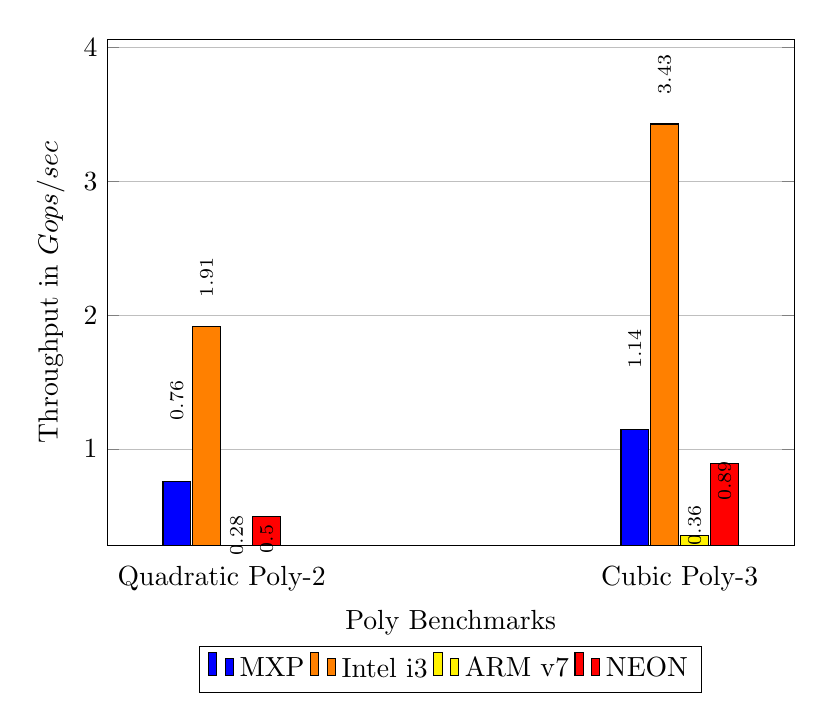
\begin{tikzpicture}
	\begin{axis}[
	width  = 0.85*\textwidth,
	height = 8cm,
	major x tick style = transparent,
	bar width=10pt,
	ymajorgrids = true,
	ylabel = {Throughput in $Gops/sec$},
	xlabel = {Poly Benchmarks},
	symbolic x coords={Quadratic Poly-2,Cubic Poly-3},
	xtick = data,
	nodes near coords,
	ybar,
	every node near coord/.append style={rotate=90, anchor=west, font=\scriptsize, xshift=0.25cm},
	scaled y ticks = false,
	enlarge y limits={upper,value=0.2},
	enlarge x limits=0.25,
	ybar=2*\pgflinewidth,
	legend cell align=left,
		legend style={
		at={(.5,-0.2)},
		anchor=north,
		legend columns=-1
		column sep=0.5ex
	}
	]
	\addplot[draw=black,fill=blue, every node near coord/.append style={xshift=0.4cm}]
	coordinates {(Quadratic Poly-2,0.758 ) (Cubic Poly-3,1.144)};
	
	\addplot[draw=black,fill=orange]
	coordinates {(Quadratic Poly-2,1.914) (Cubic Poly-3,3.43)};
	
	\addplot[draw=black,fill=yellow,every node near coord/.append style={xshift=-0.50cm}]
	coordinates {(Quadratic Poly-2,0.2819) (Cubic Poly-3,0.356)};
	
	\addplot[draw=black,fill=red, every node near coord/.append style={xshift=-0.85cm}]
	coordinates {(Quadratic Poly-2,0.4988) (Cubic Poly-3,0.8939)};
	
	\legend{MXP,Intel i3,ARM v7,NEON}
	\end{axis}
	\end{tikzpicture}
	\caption{Halfword(16-bits) level throughput(Gops/sec) for polynomial benchmarks }
	\label{poly:2}
\end{figure}

%\begin{figure}
	\centering
	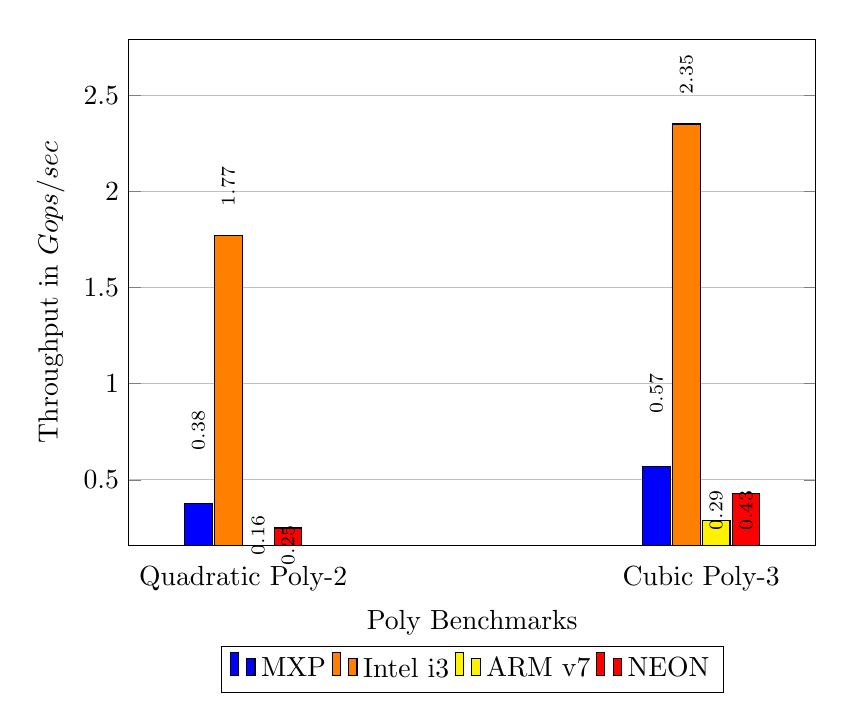
\begin{tikzpicture}
	\begin{axis}[
	width  = 0.85*\textwidth,
	height = 8cm,
	major x tick style = transparent,
	bar width=10pt,
	ymajorgrids = true,
	ylabel = {Throughput in $Gops/sec$},
	xlabel = {Poly Benchmarks},
	symbolic x coords={Quadratic Poly-2,Cubic Poly-3},
	xtick = data,
	nodes near coords,
	ybar,
	every node near coord/.append style={rotate=90, anchor=west,font=\scriptsize, xshift=0.25cm},
	scaled y ticks = false,
	enlarge y limits={upper,value=0.2},
	enlarge x limits=0.25,
	ybar=2*\pgflinewidth,
	legend cell align=left,
		legend style={
		at={(.5,-0.2)},
		anchor=north,
		legend columns=-1
		column sep=0.5ex
	}
	]
	\addplot[draw=black,fill=blue,every node near coord/.append style={xshift=0.3cm}]
	coordinates {(Quadratic Poly-2, 0.378) (Cubic Poly-3,0.571)};
	
	\addplot[draw=black,fill=orange]
	coordinates {(Quadratic Poly-2,1.77) (Cubic Poly-3,2.35)};
	
	\addplot[draw=black,fill=yellow,every node near coord/.append style={xshift=-0.50cm}]
	coordinates {(Quadratic Poly-2,0.1608) (Cubic Poly-3,0.2886)};
	
	\addplot[draw=black,fill=red,every node near coord/.append style={xshift=-0.85cm}]
	coordinates {(Quadratic Poly-2,0.2500) (Cubic Poly-3,0.4311)};
	
	\legend{MXP,Intel i3,ARM v7,NEON}
	\end{axis}
	\end{tikzpicture}
	\caption{Word(32-bits) level throughput(Gops/sec) for polynomial benchmarks }
	\label{poly:3}
\end{figure}


\pgfplotsset{
	axis background/.style={fill=none},
	tick style=black,
	tick label style=black,
	grid=both,
	xtick pos=left,
	ytick pos=left,
	tick style={
		major grid style={style=white,line width=1pt},minor grid style=white,
		tick align=outside,
	},
	minor tick num=4,
}


\begin{figure*}[!t]
\centering
\pgfplotstableread{
	0  0.23		0.55	1.41	2.32   
	1  0.37     0.47    1.54	3.33
	2  0.56     2.34    1.76	5.93 
	3  0.11    	0.58    0.69    3.80
	4  0.09    	0.68    0.91    6.96
	5  0.07    	0.44    0.62    3.49
	6  0.06		0.32	0.55	3.05
	7  0.065	0.11	0.58	2.35
	8  0.064	0.27	0.38	1.40		
}\dataset
\begin{tikzpicture}[scale=0.90]
\centering
\begin{axis}[ybar=0pt,
%enlarge x limits=0.05,
width=25cm,
x = 1.5cm,
height=6cm,
ymin=0,
ymax=8,        
ylabel={Throughput in $Gops$},
grid style={dotted,gray},
ymajorgrids=true,
nodes near coords,    
xtick=data,
bar width = 0.15,
xticklabels = {
	\strut chebyshev-byte,
	\strut mibench-byte,
	\strut qspline-byte,
	\strut fft-byte,
	\strut kmeans-byte,
	\strut mm-byte,
	\strut spmv-byte,
	\strut stencil-byte,
	\strut
	mri-byte,                               
},
x tick label style={rotate=45, anchor=north east, inner sep=0mm},
major x tick style = {opacity=0},
minor x tick num = 1,
minor tick length=1ex,
every node near coord/.append style={
        anchor=west,
        rotate=90,
        font=\tiny
},
]
\addplot[draw=black,fill=blue!90, draw opacity=1] table[x index=0,y index=1] \dataset;\label{ARM} %ano de 2013-2014
\addplot[draw=black,fill=green!90, draw opacity=1] table[x index=0,y index=2] \dataset;\label{NEON} %ano de 2012-2013
\addplot[draw=black,fill=red!90, draw opacity=1] table[x index=0,y index=3] \dataset;\label{MXP} %ano de 2012-2013
\addplot[draw=black,fill=black!90, draw opacity=1] table[x index=0,y index=4] \dataset;\label{Intel-i3} %ano de 2012-2013
\end{axis}
	\node [draw,fill=white] at (rel axis cs: 0.55,-0.40) {\shortstack[l]{
			\ref{ARM} ARM \ref{NEON} NEON \ref{MXP} MXP \ref{Intel-i3} Intel-i3}};

\end{tikzpicture}
\caption{Byte Level performance comparisons of different architectures for kernels}
\label{throughput_kernel_byte}

\end{figure*}

\pgfplotsset{
	axis background/.style={fill=none},
	tick style=black,
	tick label style=black,
	grid=both,
	xtick pos=left,
	ytick pos=left,
	tick style={
		major grid style={style=white,line width=1pt},minor grid style=white,
		tick align=outside,
	},
	minor tick num=4,
}


\begin{figure*}[!t]
\centering
\pgfplotstableread{
	0  0.19		0.51	0.70	2.18   
	1  0.35     0.78    0.77	3.73
	2  0.49     1.17    0.88	3.3 
	3  0.09    	0.28    0.34    2.01
	4  0.065    0.26    0.46    5.3
	5  0.038    0.16    0.31    3.45
	6  0.031	0.15	0.27	2.7
	7  0.053	0.12	0.29	2.57
	8  0.054	0.18	0.19	2.36		
}\dataset
\begin{tikzpicture}[scale=0.90]
\centering
\begin{axis}[ybar=0pt,
%enlarge x limits=0.05,
width=25cm,
x = 1.8cm,
height=8cm,
ymin=0,
ymax=6,        
ylabel={Throughput in $Gops$},
grid style={dotted,gray},
ymajorgrids=true,
nodes near coords,    
xtick=data,
bar width = 0.15,
xticklabels = {
	\strut chebyshev-half,
	\strut mibench-half,
	\strut qspline-half,
	\strut fft-half,
	\strut kmeans-half,
	\strut mm-half,
	\strut spmv-half,
	\strut stencil-half,
	\strut
	mri-half,                               
},
x tick label style={rotate=45, anchor=north east, inner sep=0mm},
major x tick style = {opacity=0},
minor x tick num = 1,
minor tick length=1ex,
every node near coord/.append style={
        anchor=west,
        rotate=90,
        font=\tiny
},
]
\addplot[draw=black,fill=blue!90, draw opacity=1] table[x index=0,y index=1] \dataset;\label{ARM} %ano de 2013-2014
\addplot[draw=black,fill=green!90, draw opacity=1] table[x index=0,y index=2] \dataset;\label{NEON} %ano de 2012-2013
\addplot[draw=black,fill=red!90, draw opacity=1] table[x index=0,y index=3] \dataset;\label{MXP} %ano de 2012-2013
\addplot[draw=black,fill=black!90, draw opacity=1] table[x index=0,y index=4] \dataset;\label{Intel-i3} %ano de 2012-2013
\end{axis}
	\node [draw,fill=white] at (rel axis cs: 0.55,-0.40) {\shortstack[l]{
			\ref{ARM} ARM \ref{NEON} NEON \ref{MXP} MXP \ref{Intel-i3} Intel-i3}};

\end{tikzpicture}
\caption{Halfword performance comparisons of different architectures for kernels}
\label{throughput_kernel_half}

\end{figure*}

\pgfplotsset{
	axis background/.style={fill=none},
	tick style=black,
	tick label style=black,
	grid=both,
	xtick pos=left,
	ytick pos=left,
	tick style={
		major grid style={style=white,line width=1pt},minor grid style=white,
		tick align=outside,
	},
	minor tick num=4,
}


\begin{figure*}[!t]
	\centering
	\pgfplotstableread{
		0  0.18		0.29	0.35	2.04   
		1  0.34     0.42    0.38	3.8
		2  0.29     0.46    0.44	2.3 
		3  0.08    	0.13    0.17    1.02
		4  0.03     0.09    0.15    1.24
		5  0.020    0.06    0.16    1.24
		6  0.017	0.05	0.13	1.12
		7  0.0035	0.059	0.14	1.43
		8  0.039	0.077	0.097	1.221		
	}\dataset
	\begin{tikzpicture}[scale=0.95]
	\centering
	\begin{axis}[ybar=0pt,
	%enlarge x limits=0.05,
	width=25cm,
	x = 1.8cm,
	height=8cm,
	ymin=0,
	ymax=6,        
	ylabel={Throughput in GOPS},
	grid style={dotted,gray},
	ymajorgrids=true,
	nodes near coords,    
	xtick=data,
	bar width = 0.15,
	xticklabels = {
		\strut chebyshev-word,
		\strut mibench-word,
		\strut qspline-word,
		\strut fft-word,
		\strut kmeans-word,
		\strut mm-word,
		\strut spmv-word,
		\strut stencil-word,
		\strut
		mri-word,                               
	},
	x tick label style={rotate=45, anchor=north east, inner sep=0mm},
	major x tick style = {opacity=0},
	minor x tick num = 1,
	minor tick length=1ex,
	every node near coord/.append style={
		anchor=west,
		rotate=90,
		font=\tiny
	},
	]
	\addplot[draw=black,fill=blue!90, draw opacity=1] table[x index=0,y index=1] \dataset;\label{ARM} %ano de 2013-2014
	\addplot[draw=black,fill=green!90, draw opacity=1] table[x index=0,y index=2] \dataset;\label{NEON} %ano de 2012-2013
	\addplot[draw=black,fill=red!90, draw opacity=1] table[x index=0,y index=3] \dataset;\label{MXP} %ano de 2012-2013
	\addplot[draw=black,fill=black!90, draw opacity=1] table[x index=0,y index=4] \dataset;\label{Intel-i3} %ano de 2012-2013
	\end{axis}
	\node [draw,fill=white] at (rel axis cs: 0.55,-0.40) {\shortstack[l]{
			\ref{ARM} ARM \ref{NEON} NEON \ref{MXP} MXP \ref{Intel-i3} Intel-i3}};
	
	\end{tikzpicture}
	\caption{Word Level performance comparisons of different architectures for kernels}
	\label{throughput_kernel_word}
	
\end{figure*}
\subsubsection{Throughput Analysis for filter compute kernel}

The compute kernels for second part of performance comparison which we took were the standard filter kernel. Throughput analysis for filter compute Kernels such as Chebyshev, Mibench, Sgfilter and Qspline were done.
We observed that for these benchmarks, MXP has very high throughput when it is operating at the byte(8-bits) level. MXP has very high speedups due to the superior double-buffered memory transfer optimization [3.1.3]. Table~\ref{poly:d} explains the architecture specification and the corresponding throughput obtained in terms of Gops/sec for various benchmarks. Figure~\ref{throughput_kernel_byte}, ~\ref{throughput_kernel_half} and ~\ref{throughput_kernel_word} demonstrates the average throughput (Gops/sec) obtained while operating on the word (32-bits), halfword (16- bits) and byte (8-bits) levels.
 We also observed that for a specific benchmark, the performance at the byte level was 4 times and at the halfword level was 2 times when compared with the performance at the word level for the MXP soft-vector processor. For MXP, we have the width of the data as selectable parameter.

\begin{table}[htbp]
	\centering
		\begin{adjustbox}{width=1\textwidth}
		\small
	\begin{tabular}{llllll}
		\toprule
		\textbf{Metrics} &   & \textbf{ARMv7 CPU} & \textbf{NEON (auto vector)} & \textbf{MXP} & \textbf{INTEL i3} \\
		\midrule
		\textbf{arch} &   & Scalar & SIMD unit & Vector & Scalar \\
		\textbf{clock} &   & $667 x 10^{6}Hz$ & $667 x 10^{6}Hz$ & $110 x 10^{6}Hz$ & $2 x 10^{9}Hz$ \\
		\textbf{no of lanes} &   & 1 & 2 x 32b & 1-16 x 32b & 1 \\
		&   &   & 4 x 16b & 2-32 x 16b &  \\
		&   &   & 8 x 8b & 4-64 x 8b &  \\
		&   &   &   &   &  \\
		\midrule
		 \textbf{Throughput} & \textbf{Benchmark} &   &   &   &  \\
		\midrule
		 32b(Gops/sec)/ Word   & CHEBYSHEV & 0.1832 & 0.296 & 0.354 & 2.040 \\
	 16b(Gops/sec)/Halfword &   & 0.1955 & 0.5159 & 0.7085 & 2.186 \\
		 8b(Gops/sec)/Byte &   & 0.2219 & 0.5585 & 1.41 & 2.324 \\
		   &   &   &   &   &  \\
		   &   &   &   &   &  \\
		\midrule
		 \textbf{Throughput} & \textbf{Benchmark} &   &   &   &  \\
		\midrule
		 32b(Gops/sec)/ Word   & MIBENCH & 0.3478 & 0.426 & 0.386 & 3.816 \\
		 16b(Gops/sec)/Halfword &   & 0.352 & 0.7831 & 0.773 & 6.738 \\
		 8b(Gops/sec)/Byte &   & 0.3659 & 0.460 & 1.547 & 3.338 \\
		  &   &   &   &   &  \\
		   &   &   &   &   &  \\
		\midrule
	 \textbf{Throughput} & \textbf{Benchmark} &   &   &   &  \\
		\midrule
	 32b(Gops/sec)/ Word   & QSPLINE & 0.298 & 0.4641 & 0.442 & 2.372 \\
	16b(Gops/sec)/Halfword &   & 0.493 & 1.169 & 0.88 & 13.38 \\
		 8b(Gops/sec)/Byte &   & 0.561 & 2.341 & 1.76 & 5.935 \\
		\bottomrule
	\end{tabular}%
    \end{adjustbox}%

		\caption{Throughput(Gops/sec) Analysis for Filter Benchmarks}
		\label{poly:d}%
\end{table}%
%\begin{figure}
	\centering
	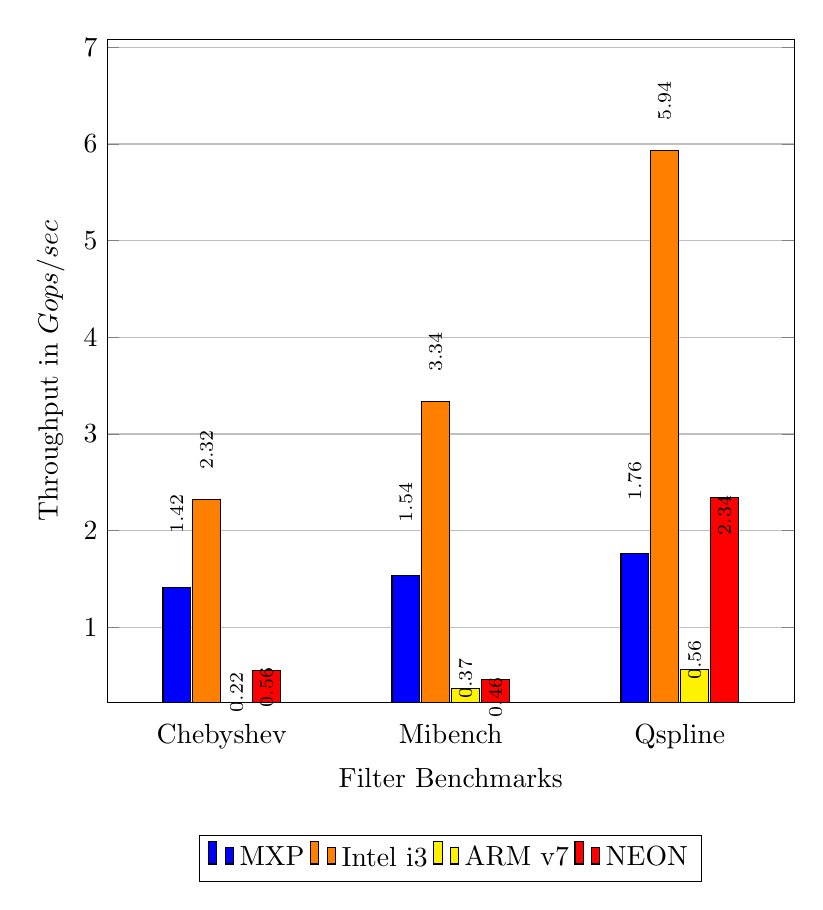
\begin{tikzpicture}
	\begin{axis}[
	width  = 0.85*\textwidth,
	height = 10cm,
	major x tick style = transparent,
	bar width=10pt,
	ymajorgrids = true,
	ylabel = {Throughput in $Gops/sec$},
	xlabel = {Filter Benchmarks},
	symbolic x coords={Chebyshev,Mibench,Qspline},
	xtick = data,
	nodes near coords,
	ybar,
	every node near coord/.append style={rotate=90, anchor=west,font=\scriptsize, xshift=0.25cm},
	scaled y ticks = false,
	enlarge y limits={upper,value=0.2},
	enlarge x limits=0.25,
	ybar=2*\pgflinewidth,
	legend cell align=left,
		legend style={
		at={(.5,-0.2)},
		anchor=north,
		legend columns=-1
		column sep=0.5ex
	}
	]
	\addplot[draw=black,fill=blue, every node near coord/.append style={xshift=.3cm}]
	coordinates {(Chebyshev, 1.417) (Mibench,1.54) (Qspline,1.76)};
	
	\addplot[draw=black,fill=orange]
	coordinates {(Chebyshev, 2.324) (Mibench,3.338) (Qspline,5.935)};
	
	\addplot[draw=black,fill=yellow, every node near coord/.append style={xshift=-0.5cm}]
	coordinates {(Chebyshev, 0.2219) (Mibench,0.3659) (Qspline,0.561)};
	
	\addplot[draw=black,fill=red, every node near coord/.append style={xshift=-0.85cm}]
	coordinates {(Chebyshev, 0.5585) (Mibench,0.460) (Qspline,2.341)};
	
	\legend{MXP,Intel i3,ARM v7,NEON}
	\end{axis}
	\end{tikzpicture}
	\caption{Byte(8-bits) level throughput(Gops/sec) for filter benchmarks }
    \label{filter:1}
\end{figure}
%
\begin{figure}
	\centering
	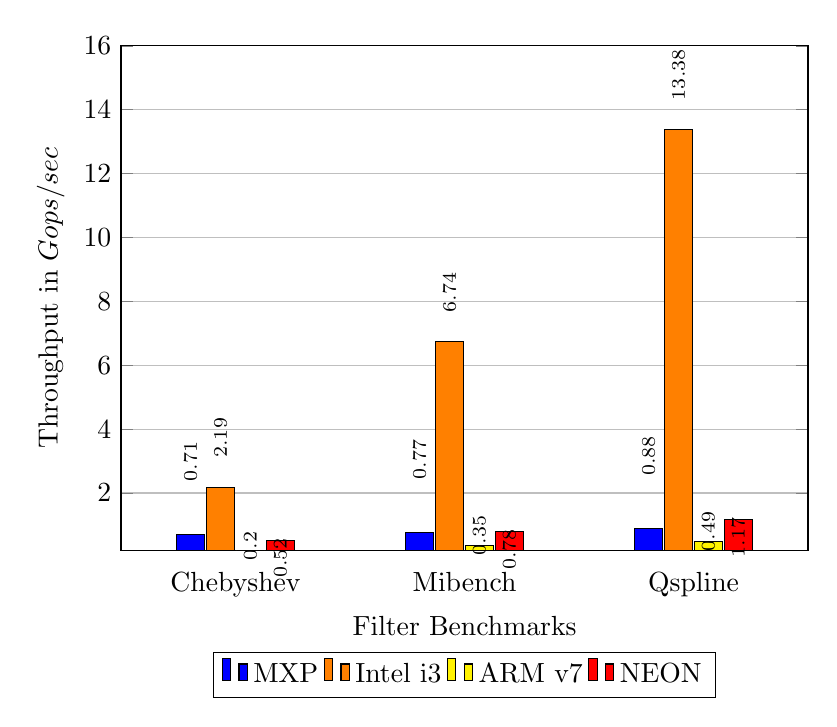
\begin{tikzpicture}
	\begin{axis}[
	width  = 0.85*\textwidth,
	height = 8cm,
	major x tick style = transparent,
	bar width=10pt,
	ymajorgrids = true,
	ylabel = {Throughput in $Gops/sec$},
	xlabel = {Filter Benchmarks},
	symbolic x coords={Chebyshev,Mibench,Qspline},
	xtick = data,
	nodes near coords,
	ybar,
	every node near coord/.append style={rotate=90, anchor=west,font=\scriptsize, xshift=0.25cm},
	scaled y ticks = false,
	enlarge y limits={upper,value=0.2},
	enlarge x limits=0.25,
	ybar=2*\pgflinewidth,
	legend cell align=left,
	legend style={
	at={(.5,-0.2)},
	anchor=north,
	legend columns=-1
	column sep=0.5ex
}
	]
	\addplot[draw=black,fill=blue,every node near coord/.append style={xshift=.3cm}]
	coordinates {(Chebyshev, 0.708) (Mibench,0.77) (Qspline,0.88)};
	
	\addplot[draw=black,fill=orange]
	coordinates {(Chebyshev, 2.186) (Mibench,6.738) (Qspline,13.38)};
	
	\addplot[draw=black,fill=yellow,every node near coord/.append style={xshift=-0.5cm}]
	coordinates {(Chebyshev, 0.1955) (Mibench,0.352) (Qspline,0.493)};
	
	\addplot[draw=black,fill=red,every node near coord/.append style={xshift=-0.85cm}]
	coordinates {(Chebyshev, 0.5159) (Mibench,0.7831) (Qspline,1.169)};
	
	\legend{MXP,Intel i3,ARM v7,NEON}
	\end{axis}
	\end{tikzpicture}
	\caption{Halfword(16-bits) level throughput(Gops/sec) for filter benchmarks }
	\label{filter:2}
\end{figure}
%\begin{figure}
	\centering
	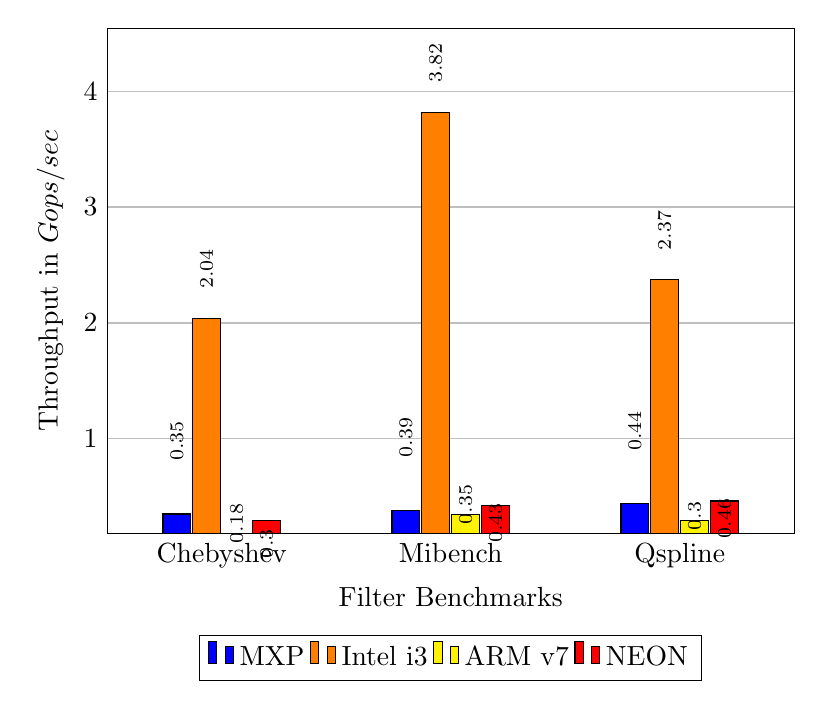
\begin{tikzpicture}
	\begin{axis}[
	width  = 0.85*\textwidth,
	height = 8cm,
	major x tick style = transparent,
	bar width=10pt,
	ymajorgrids = true,
	ylabel = {Throughput in $Gops/sec$},
	xlabel = {Filter Benchmarks},
	symbolic x coords={Chebyshev,Mibench,Qspline},
	major tick length=0cm,
	xtick = data,
	nodes near coords,
	ybar,
	every node near coord/.append style={rotate=90, anchor=west,font=\scriptsize, xshift=0.25cm},
	scaled y ticks = false,
	enlarge y limits={upper,value=0.2},
	enlarge x limits=0.25,
	ybar=2*\pgflinewidth,
	legend cell align=left,
	legend style={
	at={(.5,-0.2)},
	anchor=north,
	legend columns=-1
	column sep=0.5ex
}
	]
	\addplot[draw=black,fill=blue,every node near coord/.append style={xshift=.3cm}]
	coordinates {(Chebyshev, 0.352) (Mibench,0.385) (Qspline,0.44)};
	
	\addplot[draw=black,fill=orange]
	coordinates {(Chebyshev, 2.040) (Mibench,3.816) (Qspline,2.372)};
	
	\addplot[draw=black,fill=yellow, every node near coord/.append style={xshift=-0.5cm}]
	coordinates {(Chebyshev, 0.1832) (Mibench,0.3478) (Qspline,0.298)};
	
	\addplot[draw=black,fill=red, every node near coord/.append style={xshift=-.85cm}]
	coordinates {(Chebyshev, 0.296) (Mibench,0.426) (Qspline,0.4641)};
	
	\legend{MXP,Intel i3,ARM v7,NEON}
	\end{axis}
	\end{tikzpicture}
	\caption{Word(32-bits) level throughput(Gops/sec) for filter benchmarks }
	\label{filter:3}
\end{figure}
%
\pgfplotsset{
	axis background/.style={fill=none},
	tick style=black,
	tick label style=black,
	grid=both,
	xtick pos=left,
	ytick pos=left,
	tick style={
		major grid style={style=white,line width=1pt},minor grid style=white,
		tick align=outside,
	},
	minor tick num=4,
}


\begin{figure*}[!t]
\centering
\pgfplotstableread{
	0  0.23		0.55	1.41	2.32   
	1  0.37     0.47    1.54	3.33
	2  0.56     2.34    1.76	5.93 
	3  0.11    	0.58    0.69    3.80
	4  0.09    	0.68    0.91    6.96
	5  0.07    	0.44    0.62    3.49
	6  0.06		0.32	0.55	3.05
	7  0.065	0.11	0.58	2.35
	8  0.064	0.27	0.38	1.40		
}\dataset
\begin{tikzpicture}[scale=0.90]
\centering
\begin{axis}[ybar=0pt,
%enlarge x limits=0.05,
width=25cm,
x = 1.5cm,
height=6cm,
ymin=0,
ymax=8,        
ylabel={Throughput in $Gops$},
grid style={dotted,gray},
ymajorgrids=true,
nodes near coords,    
xtick=data,
bar width = 0.15,
xticklabels = {
	\strut chebyshev-byte,
	\strut mibench-byte,
	\strut qspline-byte,
	\strut fft-byte,
	\strut kmeans-byte,
	\strut mm-byte,
	\strut spmv-byte,
	\strut stencil-byte,
	\strut
	mri-byte,                               
},
x tick label style={rotate=45, anchor=north east, inner sep=0mm},
major x tick style = {opacity=0},
minor x tick num = 1,
minor tick length=1ex,
every node near coord/.append style={
        anchor=west,
        rotate=90,
        font=\tiny
},
]
\addplot[draw=black,fill=blue!90, draw opacity=1] table[x index=0,y index=1] \dataset;\label{ARM} %ano de 2013-2014
\addplot[draw=black,fill=green!90, draw opacity=1] table[x index=0,y index=2] \dataset;\label{NEON} %ano de 2012-2013
\addplot[draw=black,fill=red!90, draw opacity=1] table[x index=0,y index=3] \dataset;\label{MXP} %ano de 2012-2013
\addplot[draw=black,fill=black!90, draw opacity=1] table[x index=0,y index=4] \dataset;\label{Intel-i3} %ano de 2012-2013
\end{axis}
	\node [draw,fill=white] at (rel axis cs: 0.55,-0.40) {\shortstack[l]{
			\ref{ARM} ARM \ref{NEON} NEON \ref{MXP} MXP \ref{Intel-i3} Intel-i3}};

\end{tikzpicture}
\caption{Byte Level performance comparisons of different architectures for kernels}
\label{throughput_kernel_byte}

\end{figure*}
%
\pgfplotsset{
	axis background/.style={fill=none},
	tick style=black,
	tick label style=black,
	grid=both,
	xtick pos=left,
	ytick pos=left,
	tick style={
		major grid style={style=white,line width=1pt},minor grid style=white,
		tick align=outside,
	},
	minor tick num=4,
}


\begin{figure*}[!t]
\centering
\pgfplotstableread{
	0  0.19		0.51	0.70	2.18   
	1  0.35     0.78    0.77	3.73
	2  0.49     1.17    0.88	3.3 
	3  0.09    	0.28    0.34    2.01
	4  0.065    0.26    0.46    5.3
	5  0.038    0.16    0.31    3.45
	6  0.031	0.15	0.27	2.7
	7  0.053	0.12	0.29	2.57
	8  0.054	0.18	0.19	2.36		
}\dataset
\begin{tikzpicture}[scale=0.90]
\centering
\begin{axis}[ybar=0pt,
%enlarge x limits=0.05,
width=25cm,
x = 1.8cm,
height=8cm,
ymin=0,
ymax=6,        
ylabel={Throughput in $Gops$},
grid style={dotted,gray},
ymajorgrids=true,
nodes near coords,    
xtick=data,
bar width = 0.15,
xticklabels = {
	\strut chebyshev-half,
	\strut mibench-half,
	\strut qspline-half,
	\strut fft-half,
	\strut kmeans-half,
	\strut mm-half,
	\strut spmv-half,
	\strut stencil-half,
	\strut
	mri-half,                               
},
x tick label style={rotate=45, anchor=north east, inner sep=0mm},
major x tick style = {opacity=0},
minor x tick num = 1,
minor tick length=1ex,
every node near coord/.append style={
        anchor=west,
        rotate=90,
        font=\tiny
},
]
\addplot[draw=black,fill=blue!90, draw opacity=1] table[x index=0,y index=1] \dataset;\label{ARM} %ano de 2013-2014
\addplot[draw=black,fill=green!90, draw opacity=1] table[x index=0,y index=2] \dataset;\label{NEON} %ano de 2012-2013
\addplot[draw=black,fill=red!90, draw opacity=1] table[x index=0,y index=3] \dataset;\label{MXP} %ano de 2012-2013
\addplot[draw=black,fill=black!90, draw opacity=1] table[x index=0,y index=4] \dataset;\label{Intel-i3} %ano de 2012-2013
\end{axis}
	\node [draw,fill=white] at (rel axis cs: 0.55,-0.40) {\shortstack[l]{
			\ref{ARM} ARM \ref{NEON} NEON \ref{MXP} MXP \ref{Intel-i3} Intel-i3}};

\end{tikzpicture}
\caption{Halfword performance comparisons of different architectures for kernels}
\label{throughput_kernel_half}

\end{figure*}
%
\pgfplotsset{
	axis background/.style={fill=none},
	tick style=black,
	tick label style=black,
	grid=both,
	xtick pos=left,
	ytick pos=left,
	tick style={
		major grid style={style=white,line width=1pt},minor grid style=white,
		tick align=outside,
	},
	minor tick num=4,
}


\begin{figure*}[!t]
	\centering
	\pgfplotstableread{
		0  0.18		0.29	0.35	2.04   
		1  0.34     0.42    0.38	3.8
		2  0.29     0.46    0.44	2.3 
		3  0.08    	0.13    0.17    1.02
		4  0.03     0.09    0.15    1.24
		5  0.020    0.06    0.16    1.24
		6  0.017	0.05	0.13	1.12
		7  0.0035	0.059	0.14	1.43
		8  0.039	0.077	0.097	1.221		
	}\dataset
	\begin{tikzpicture}[scale=0.95]
	\centering
	\begin{axis}[ybar=0pt,
	%enlarge x limits=0.05,
	width=25cm,
	x = 1.8cm,
	height=8cm,
	ymin=0,
	ymax=6,        
	ylabel={Throughput in GOPS},
	grid style={dotted,gray},
	ymajorgrids=true,
	nodes near coords,    
	xtick=data,
	bar width = 0.15,
	xticklabels = {
		\strut chebyshev-word,
		\strut mibench-word,
		\strut qspline-word,
		\strut fft-word,
		\strut kmeans-word,
		\strut mm-word,
		\strut spmv-word,
		\strut stencil-word,
		\strut
		mri-word,                               
	},
	x tick label style={rotate=45, anchor=north east, inner sep=0mm},
	major x tick style = {opacity=0},
	minor x tick num = 1,
	minor tick length=1ex,
	every node near coord/.append style={
		anchor=west,
		rotate=90,
		font=\tiny
	},
	]
	\addplot[draw=black,fill=blue!90, draw opacity=1] table[x index=0,y index=1] \dataset;\label{ARM} %ano de 2013-2014
	\addplot[draw=black,fill=green!90, draw opacity=1] table[x index=0,y index=2] \dataset;\label{NEON} %ano de 2012-2013
	\addplot[draw=black,fill=red!90, draw opacity=1] table[x index=0,y index=3] \dataset;\label{MXP} %ano de 2012-2013
	\addplot[draw=black,fill=black!90, draw opacity=1] table[x index=0,y index=4] \dataset;\label{Intel-i3} %ano de 2012-2013
	\end{axis}
	\node [draw,fill=white] at (rel axis cs: 0.55,-0.40) {\shortstack[l]{
			\ref{ARM} ARM \ref{NEON} NEON \ref{MXP} MXP \ref{Intel-i3} Intel-i3}};
	
	\end{tikzpicture}
	\caption{Word Level performance comparisons of different architectures for kernels}
	\label{throughput_kernel_word}
	
\end{figure*}

\subsubsection{Throughput Analysis for Standard kernels}

As a third part of performance comparison work, we took various benchmarks such as FFT, KMEANS, MM, SPMV, STENCIL and MRI which are the standard compute kernels. We observed that for these compute kernels, MXP has high throughput. MXP has very high speedups due to the superior double-buffered memory transfer optimization [3.1.3]. Table~\ref{poly:a} explains the architecture specification and the corresponding throughput obtained in terms of Gops/sec for various benchmarks. Figure~\ref{throughput_kernel_byte}, ~\ref{throughput_kernel_half}and ~\ref{throughput_kernel_word} demonstrates the average throughput (Gops/sec) obtained while operating on the word (32-bits), halfword (16- bits) and byte (8-bits) levels.

\begin{table}[htbp]
	\centering
    	\begin{adjustbox}{width=.8\textwidth}
    	\small
	\begin{tabular}{llllll}
		\toprule
		\textbf{Metrics} &   & \textbf{ARMv7 CPU} & \textbf{NEON (auto vector)} & \textbf{MXP} & \textbf{INTEL i3} \\
		\midrule
		\textbf{arch} &   & Scalar & SIMD unit & Vector & Scalar \\
		\textbf{clock} &   & $667 X 10^{6}Hz$ & $667 X 10^{6}Hz$ & $110 X 10^{6}Hz$ & $2 X 10^{9}Hz$ \\
		\textbf{no of lanes} &   & 1 & 2 x 32b & 1-16 x 32b & 1 \\
		&   &   & 4 x 16b & 2-32 x 16b &  \\
		&   &   & 8 x 8b & 4-64 x 8b &  \\
		\midrule
		  \textbf{Throughput} & \textbf{Benchmark} &   &   &   &  \\
		\midrule
		  32b(Gops/sec)/ Word   & FFT & 0.0867 & 0.137 & 0.174 & 1.0283 \\
		  16b(Gops/sec)/Halfword &   & 0.0937 & 0.2887 & 0.349 & 2.01 \\
		  8b(Gops/sec)/Byte &   & 0.1042 & 0.5833 & 0.6995 & 3.809 \\
		    &   &   &   &   &  \\
		\midrule
		  \textbf{Throughput} & \textbf{Benchmark} &   &   &   &  \\
		\midrule
		  32b(Gops/sec)/ Word   & KMEANS & 0.03174 & 0.09083 & 0.2285 & 1.918 \\
		  16b(Gops/sec)/Halfword &   & 0.06582 & 0.257 & 0.457 & 5.301 \\
		  8b(Gops/sec)/Byte &   & 0.0986 & 0.689 & 0.9143 & 6.96 \\
		    &   &   &   &   &  \\
		\midrule
		  \textbf{Throughput} & \textbf{Benchmark} &   &   &   &  \\
		\midrule
		  32b(Gops/sec)/ Word   & MM & 0.02015 & 0.06009 & 0.156 & 1.24 \\
		  16b(Gops/sec)/Halfword &   & 0.03806 & 0.165 & 0.3136 & 3.456 \\
		  8b(Gops/sec)/Byte &   & 0.0667 & 0.443 & 0.627 & 3.495 \\
		    &   &   &   &   &  \\
		\midrule
		  \textbf{Throughput} & \textbf{Benchmark} &   &   &   &  \\
		\midrule
		  32b(Gops/sec)/ Word   & SPMV & 0.01680 & 0.0532 & 0.1399 & 1.126 \\
		  16b(Gops/sec)/Halfword &   & 0.0307 & 0.1529 & 0.279 & 2.696 \\
		  8b(Gops/sec)/Byte &   & 0.061 & 0.391 & 0.5596 & 3.05 \\
		    &   &   &   &   &  \\
		\midrule
		  \textbf{Throughput} & \textbf{Benchmark} &   &   &   &  \\
		\midrule
		  32b(Gops/sec)/ Word   & STENCIL & 0.03589 & 0.05866 & 0.14 & 1.437 \\
		  16b(Gops/sec)/Halfword &   & 0.0534 & 0.1146 & 0.29 & 2.57 \\
		  8b(Gops/sec)/Byte &   & 0.0651 & 0.1162 & 0.589 & 2.35 \\
		    &   &   &   &   &  \\
		\midrule
		  \textbf{Throughput} & \textbf{Benchmark} &   &   &   &  \\
		\midrule
		  32b(Gops/sec)/ Word   & MRI & 0.039 & 0.077 & 0.097 & 1.221 \\
		  16b(Gops/sec)/Halfword &   & 0.0537 & 0.183 & 0.194 & 2.36 \\
		  8b(Gops/sec)/Byte &   & 0.064 & 0.277 & 0.388 & 1.406 \\
		\bottomrule
	\end{tabular}%
\end{adjustbox}%
	\caption{Throughput(Gops/sec) Analysis for Standard Compute Kernels}
		\label{poly:a}%
\end{table}%
%
\begin{figure}
	\centering
	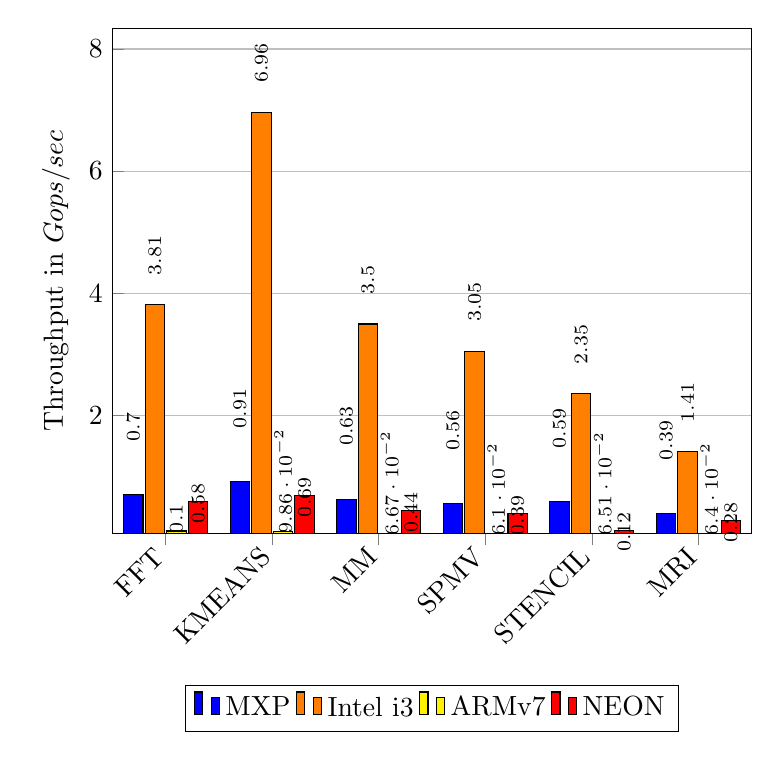
\begin{tikzpicture}
	\begin{axis}[
	width  = 0.8*\textwidth,
	height = 8cm,
	xtick pos=left,
    ytick pos=left,
%	major x tick style = transparent,
	x tick label style={rotate=45, anchor=east, align=right,text width=2cm},
	bar width=7pt,
	ymajorgrids = true,
	ylabel = {Throughput in $Gops/sec$},
	symbolic x coords={FFT,KMEANS,MM,SPMV,STENCIL,MRI},
	xtick = data,
	nodes near coords,
	ybar,
	every node near coord/.append style={rotate=90, anchor=west,font=\scriptsize, xshift=0.25cm},
	scaled y ticks = false,
	enlarge y limits={upper,value=0.2},
%	enlarge x limits=0.25,
	ybar=2*\pgflinewidth,
	legend cell align=left,
	legend style={
	at={(.5,-0.3)},
	anchor=north,
	legend columns=-1
	column sep=0.5ex
}
	]
	\addplot[draw=black,fill=blue,every node near coord/.append style={xshift=0.3cm}]
	coordinates {(FFT, 0.69951) (KMEANS,0.914) (MM,0.627) (SPMV,0.559) (STENCIL,0.589) (MRI,0.388)};
	
	\addplot[draw=black,fill=orange]
	coordinates  {(FFT,3.809) (KMEANS,6.96) (MM,3.495) (SPMV,3.05) (STENCIL,2.35) (MRI,1.406)};
	
	\addplot[draw=black,fill=yellow,every node near coord/.append style={xshift=-0.4cm}]
	coordinates  {(FFT,0.1042) (KMEANS,0.0986) (MM,0.0667) (SPMV,0.061) (STENCIL,0.0651) (MRI,0.064)};
	
	\addplot[draw=black,fill=red,every node near coord/.append style={xshift=-0.65cm}]
	coordinates {(FFT, 0.5833) (KMEANS,0.689) (MM,0.443) (SPMV,0.391) (STENCIL,0.1162) (MRI,0.277)};
	
	\legend{MXP,Intel i3,ARMv7,NEON}
	\end{axis}
	\end{tikzpicture}
	\caption{Byte(8-bits) level throughput(Gops/sec) for compute Kernels}
	\label{kernel:1}
\end{figure}


%
\begin{figure}
	\centering
	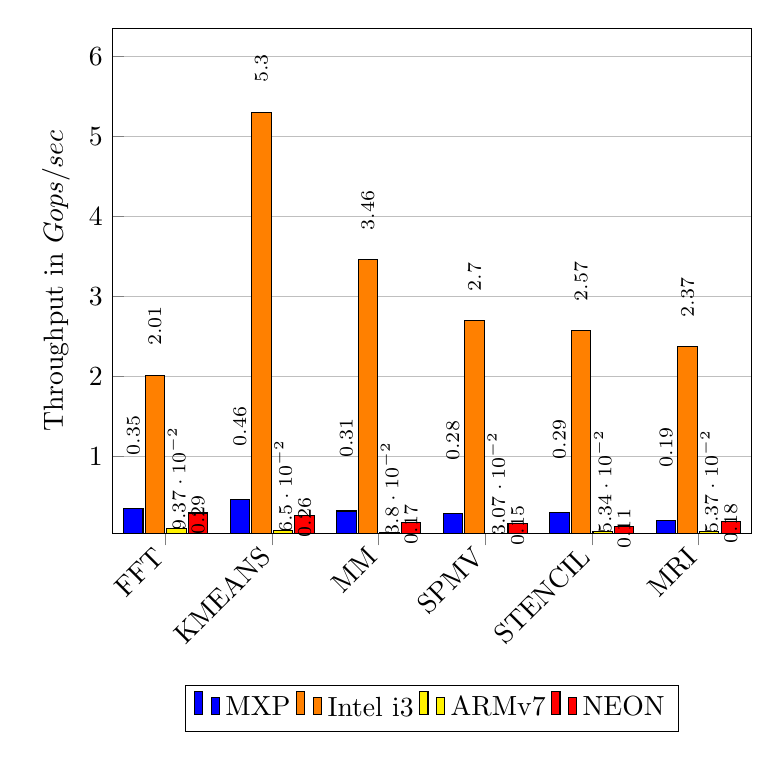
\begin{tikzpicture}
	\begin{axis}[
	width  = 0.8*\textwidth,
	height = 8cm,
	xtick pos=left,
	ytick pos=left,
%	major x tick style = transparent,
	x tick label style={rotate=45, anchor=east, align=right,text width=2cm},
	bar width=7pt,
	ymajorgrids = true,
	ylabel = {Throughput in $Gops/sec$},
	symbolic x coords={FFT,KMEANS,MM,SPMV,STENCIL,MRI},
	xtick = data,
	nodes near coords,
	ybar,
	every node near coord/.append style={rotate=90, anchor=west,font=\scriptsize, xshift=0.25cm},
	scaled y ticks = false,
	enlarge y limits={upper,value=0.2},
%	enlarge x limits=0.25,
	ybar=2*\pgflinewidth,
	legend cell align=left,
	legend style={
		at={(.5,-0.3)},
		anchor=north,
		legend columns=-1
		column sep=0.5ex
	}
	]
	\addplot[draw=black,fill=blue,every node near coord/.append style={xshift=.3cm}]
	coordinates {(FFT, 0.349) (KMEANS,0.457) (MM,0.313) (SPMV,0.2798) (STENCIL,0.294) (MRI,0.194)};
	
	\addplot[draw=black,fill=orange]
	coordinates  {(FFT, 2.01) (KMEANS,5.301) (MM,3.456) (SPMV,2.696) (STENCIL,2.57) (MRI,2.368)};
	
	\addplot[draw=black,fill=yellow,every node near coord/.append style={xshift=-0.4cm}]
	coordinates  {(FFT,0.0937) (KMEANS,0.065) (MM,0.038) (SPMV,0.0307) (STENCIL,0.0534) (MRI,0.0537)};
	
	\addplot[draw=black,fill=red,every node near coord/.append style={xshift=-0.65cm}]
	coordinates {(FFT, 0.2887) (KMEANS,0.257) (MM,0.165) (SPMV,0.1529) (STENCIL,0.1146) (MRI,0.1839)};
	
	\legend{MXP,Intel i3,ARMv7,NEON}
	\end{axis}
	\end{tikzpicture}
	\caption{Halfword(16-bits) level throughput(Gops/sec) for compute Kernels}
	\label{kernel:2}
\end{figure}
%
\begin{figure}
	\centering
	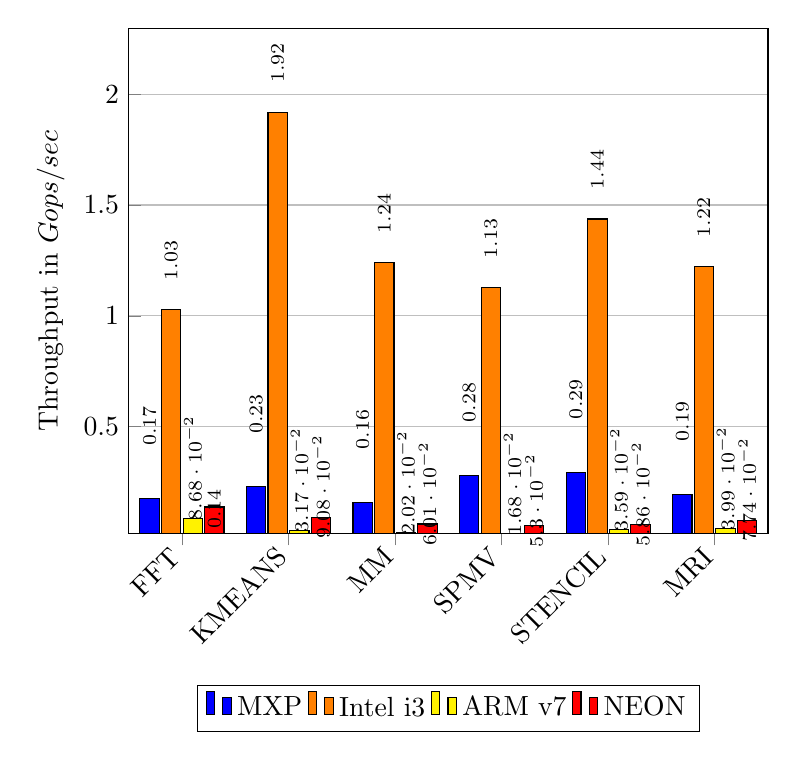
\begin{tikzpicture}
	\begin{axis}[
	width  = 0.8*\textwidth,
	height = 8cm,
	xtick pos=left,
	ytick pos=left,
%	major x tick style = transparent,
	x tick label style={rotate=45, anchor=east, align=right,text width=2cm},
	bar width=7pt,
	ymajorgrids = true,
	ylabel = {Throughput in $Gops/sec$},
	symbolic x coords={FFT,KMEANS,MM,SPMV,STENCIL,MRI},
	xtick = data,
	nodes near coords,
	ybar,
	every node near coord/.append style={rotate=90, anchor=west,font=\scriptsize, xshift=0.25cm},
	scaled y ticks = false,
	enlarge y limits={upper,value=0.2},
%	enlarge x limits=0.25,
	ybar=2*\pgflinewidth,
	legend cell align=left,
	legend style={
	at={(.5,-0.3)},
	anchor=north,
	legend columns=-1
	column sep=0.5ex
}
	]
	\addplot[draw=black,fill=blue,every node near coord/.append style={xshift=0.3cm}]
	coordinates {(FFT,0.174) (KMEANS,0.2285) (MM,0.1567) (SPMV,0.2798) (STENCIL,0.2945) (MRI,0.194)};
	
	\addplot[draw=black,fill=orange]
	coordinates  {(FFT,1.0283) (KMEANS,1.918) (MM,1.24) (SPMV,1.126) (STENCIL,1.437) (MRI,1.2211)};
	
	\addplot[draw=black,fill=yellow,every node near coord/.append style={xshift=-0.4cm}]
	coordinates  {(FFT, 0.08677) (KMEANS,0.03174) (MM,0.02015) (SPMV,0.01680) (STENCIL,0.03589) (MRI,0.0399)};
	
	\addplot[draw=black,fill=red,every node near coord/.append style={xshift=-0.65cm}]
	coordinates {(FFT, 0.13705) (KMEANS,0.0908) (MM,0.06009) (SPMV,0.053) (STENCIL,0.0586) (MRI,0.07735)};
	
	\legend{MXP,Intel i3,ARM v7,NEON}
	\end{axis}
	\end{tikzpicture}
	\caption{Word(32-bits) level throughput(Gops/sec) for compute Kernels}
	\label{kernel:3}
\end{figure}

\subsubsection{Throughput Analysis for Linear Algebra Kernel}

We accelerate two linear algebra kernels namely atax and bicg using MXP overlay. We change the default data type which is double to integer for the computations to have proper comparison analysis about the speedup. We accelerate the kernel for a small dataset with size of matrix 500x500 and for standard dataset size of matrix 4000x4000. The speedup obtained using MXP is as shown in the below table~\ref{lin:a}. We observed that MXP provide high speedup for small as well as standard dataset. For the BiCG kernel, MXP provide speedup of 3 for the small dataset and 3.25 for the standard dataset when compared with the embedded hard processor ARM v7. For ATAX compute kernel, speedup was observed to be 5.62 for the small dataset and 4.63 for standard dataset.



% Table generated by Excel2LaTeX from sheet 'Sheet1'
\begin{table}[htbp]
	\centering
	\begin{adjustbox}{width= .8\textwidth}
		\small
		\begin{tabular}{rrrrr}
			\toprule
			\multicolumn{1}{l}{\textbf{Metrics}} &   & \multicolumn{1}{l}{\textbf{ARMv7 CPU}} & \multicolumn{1}{l}{\textbf{MXP}} & \multicolumn{1}{l}{\textbf{NEON(auto vector)}} \\
			\midrule
			\multicolumn{1}{l}{\textbf{uarch}} &   & \multicolumn{1}{l}{Scalar} & \multicolumn{1}{l}{Soft vector} & \multicolumn{1}{l}{SIMD unit} \\
			\multicolumn{1}{l}{\textbf{Clock}} &   & \multicolumn{1}{l}{667 Mhz} & \multicolumn{1}{l}{110 Mhz} & \multicolumn{1}{l}{667 Mhz} \\
			\multicolumn{1}{l}{\textbf{No of Lanes}} &   & \multicolumn{1}{l}{1} & \multicolumn{1}{l}{1-16 X32b} & \multicolumn{1}{l}{2 X32b} \\
			&   &   & \multicolumn{1}{l}{2-32 X16b} & \multicolumn{1}{l}{4 X16b} \\
			&   &   & \multicolumn{1}{l}{4-64 X8b} & \multicolumn{1}{l}{8 X8b} \\
			\midrule
			\multicolumn{1}{l}{\textbf{Runtime (ms)}} & \multicolumn{1}{l}{\textbf{Benchmark}} &   &   &  \\
			\midrule
			\multicolumn{1}{l}{500 X 500 (small dataset)} & \multicolumn{1}{l}{BiCG} & \multicolumn{1}{l}{5.935} & \multicolumn{1}{l}{1.972} & \multicolumn{1}{l}{5.89} \\
			&   &   &   &  \\
			\multicolumn{1}{l}{4000 X 4000 (standard dataset)} &   & \multicolumn{1}{l}{234.69} & \multicolumn{1}{l}{72.033} & \multicolumn{1}{l}{216.26} \\
			&   &   &   &  \\
			\midrule
			\multicolumn{1}{l}{\textbf{Runtime (ms)}} & \multicolumn{1}{l}{\textbf{Benchmark}} &   &   &  \\
			\midrule
			\multicolumn{1}{l}{500 X 500 (small dataset)} & \multicolumn{1}{l}{ATAX} & \multicolumn{1}{l}{6.598} & \multicolumn{1}{l}{1.172} & \multicolumn{1}{l}{6.581} \\
			&   &   &   &  \\
			\multicolumn{1}{l}{4000 X 4000 (standard dataset)} &   & \multicolumn{1}{l}{486.96} & \multicolumn{1}{l}{105.303} & \multicolumn{1}{l}{483.99} \\
			&   &   &   &  \\
			\bottomrule
		\end{tabular}%
	\end{adjustbox}%
	\caption{Throughput(Gops/sec) Analysis for Linear Algebra kernel}
	\label{lin:a}%	
\end{table}%


    
    
    \subsubsection{Speedup Analysis w.r.t ARM cortex A9}
    Speedup analysis for MXP, SIMD NEON and INTEL i3 was obtained taking ARM Cortex A9 as the reference processor. The DFG processing for the various kernels on MXP is summarized in this section. The speedup factors were calculated for standard kernels at the byte, halfword and the word level. The analysis shows that when we are operating at the byte level the MXP provides the four times parallelism and hence is supposed to give high speedup as compared to other processors. Figure~\ref{speedup:1} demonstrates the byte level speedup obtained with respect to the ARM cortex A9 processor. It can be inferred that the MXP provides high speedup for the kernel with much more computation as MXP make use of the overlapping of communication and computation feature to hide the time incurred in transferring the data. Figure~\ref{speedup:2} and Figure~\ref{speedup:3} demonstrates the halfword and the word level speedup obtained with respect to the ARM cortex A9 processor. With respect to these graphs it can be observed that the INTEL i3 processor have some better speedup for kernels requiring high computation.
  
  \section{Compute Kernel Code}
  
  Runtime and Throughput calculation application for all the compute kernels can be found from the below given repository:
  
  Github Link : \url{https://github.com/AdhikariSaurabh/mxpbenchmarks/polyresults}
  
  
\begin{figure}
	\centering
	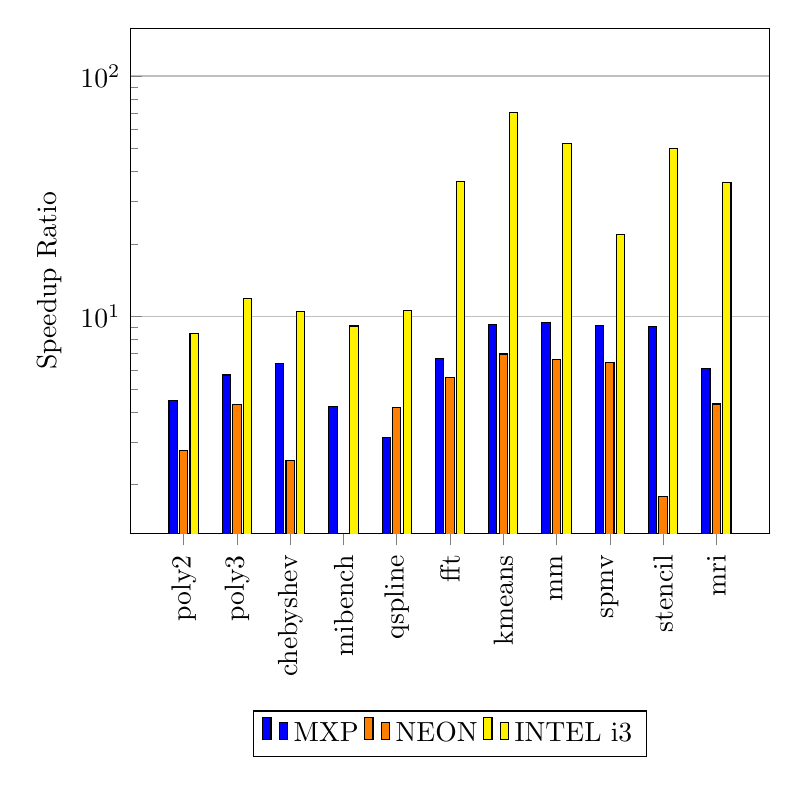
\begin{tikzpicture}
	\begin{semilogyaxis}[
	width  = 0.8*\textwidth,
	height = 8cm,
	xtick pos=left,
	ytick pos=left,
	%	major x tick style = transparent,
	x tick label style={rotate=90, anchor=east, align=right,text width=2cm},
	bar width=3pt,
	ymajorgrids = true,
	ylabel = {Speedup Ratio},
	symbolic x coords={poly2,poly3,chebyshev,mibench,qspline,fft,kmeans,mm,spmv,stencil,mri},
	xtick = data,
%	nodes near coords,
%	ybar,
%	every node near coord/.append style={rotate=90, anchor=west,font=\tiny, xshift=0.25cm},
	%	nodes near coords,
	%	ybar,
	%	every node near coord/.append style={rotate=90, anchor=west,font=\scriptsize},
	scaled y ticks = false,
	enlarge y limits={upper,value=0.2},
	%test
	%	enlarge x limits=0.25,
	ybar=2*\pgflinewidth,
	legend cell align=left,
	legend style={
		at={(.5,-0.35)},
		anchor=north,
		legend columns=-1
		column sep=0.5ex
	}
	]
	\addplot[draw=black,fill=blue]
	coordinates {(poly2,4.49) (poly3,5.709) (chebyshev,6.386) (mibench,4.22) (qspline,3.13) (fft,6.71) (kmeans,9.26) (mm,9.400) (spmv,9.1737) (stencil,9.0538) (mri,6.059) };
	
	\addplot[draw=black,fill=orange]
	coordinates	{(poly2,2.775 ) (poly3,4.32) (chebyshev,2.51) (mibench,1.25) (qspline,4.17) (fft,5.597) (kmeans,6.983) (mm,6.641) (spmv,6.4098) (stencil,1.784) (mri,4.326) };
	
	\addplot[draw=black,fill=yellow]
	coordinates	{(poly2,8.469 ) (poly3,11.834) (chebyshev,10.47) (mibench,9.122) (qspline,10.57) (fft,36.55) (kmeans,70.54) (mm,52.39) (spmv,21.96) (stencil,50) (mri,36.098) };
	
	\legend{MXP,NEON,INTEL i3}
	\end{semilogyaxis}	
	\end{tikzpicture}
	\caption{Byte level Speedup Analysis w.r.t ARMv7 for  different benchmarks.}
	\label{speedup:1}
\end{figure}

   
 
 \begin{figure}
 	\centering
 	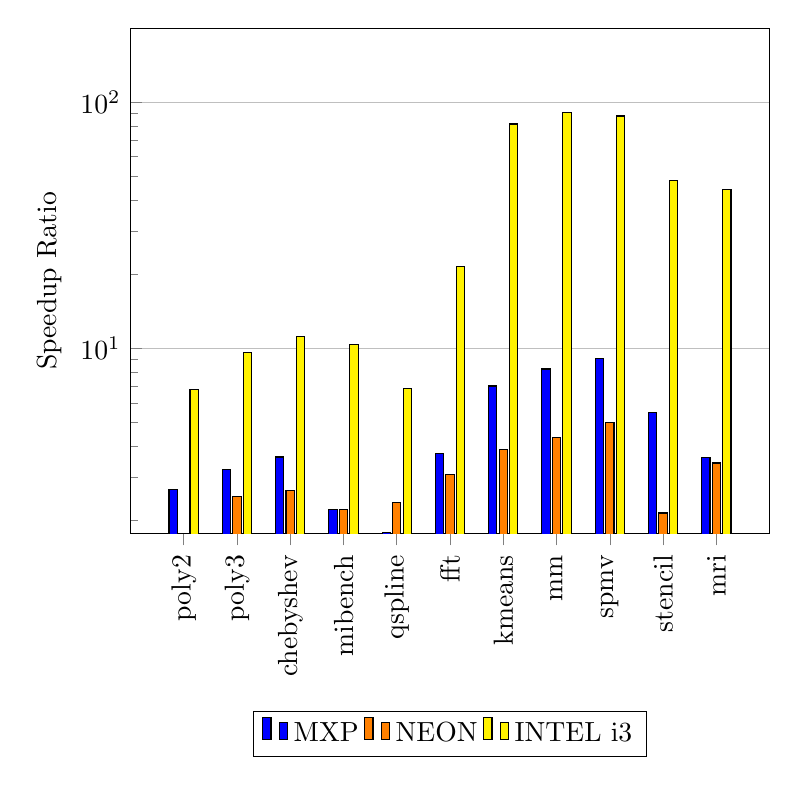
\begin{tikzpicture}
 	\begin{semilogyaxis}[
 	width  = 0.8*\textwidth,
 	height = 8cm,
 	xtick pos=left,
 	ytick pos=left,
 	%	major x tick style = transparent,
 	x tick label style={rotate=90, anchor=east, align=right,text width=2cm},
 	bar width=3pt,
 	ymajorgrids = true,
 	ylabel = {Speedup Ratio},
 	symbolic x coords={poly2,poly3,chebyshev,mibench,qspline,fft,kmeans,mm,spmv,stencil,mri},
 	xtick = data,
% 	nodes near coords,
% 	ybar,
% 	every node near coord/.append style={rotate=90, anchor=west,font=\tiny},
 	scaled y ticks = false,
 	enlarge y limits={upper,value=0.2},
 	%test
 	%	enlarge x limits=0.25,
 	ybar=2*\pgflinewidth,
 	legend cell align=left,
 	legend style={
 		at={(.5,-0.35)},
 		anchor=north,
 		legend columns=-1
 		column sep=0.5ex
 	}
 	]
 	\addplot[draw=black,fill=blue]
 	coordinates {(poly2,2.683) (poly3,3.21) (chebyshev,3.62) (mibench,2.216) (qspline,1.784) (fft,3.729) (kmeans,7.033) (mm,8.25) (spmv,9.11) (stencil,5.51) (mri,3.61) };
 	
 	\addplot[draw=black,fill=orange]
 	coordinates	{(poly2,1.769 ) (poly3,2.51) (chebyshev,2.638) (mibench,2.224) (qspline,2.3711) (fft,3.0811) (kmeans,3.90) (mm,4.335) (spmv,4.980) (stencil,2.146) (mri,3.424) };
 	
 	\addplot[draw=black,fill=yellow]
 	coordinates	{(poly2,6.78 ) (poly3,9.634) (chebyshev,11.18) (mibench,10.38) (qspline,6.855) (fft,21.45) (kmeans,81.5) (mm,90.8) (spmv,87.81) (stencil,48.12) (mri,44) };
 	
 	\legend{MXP,NEON,INTEL i3}
 	\end{semilogyaxis}	
 	\end{tikzpicture}
 	\caption{Half Word level Speedup Analysis w.r.t ARMv7 for  different benchmarks.}
 	\label{speedup:2}
 \end{figure}
 

  

\begin{figure}
	\centering
	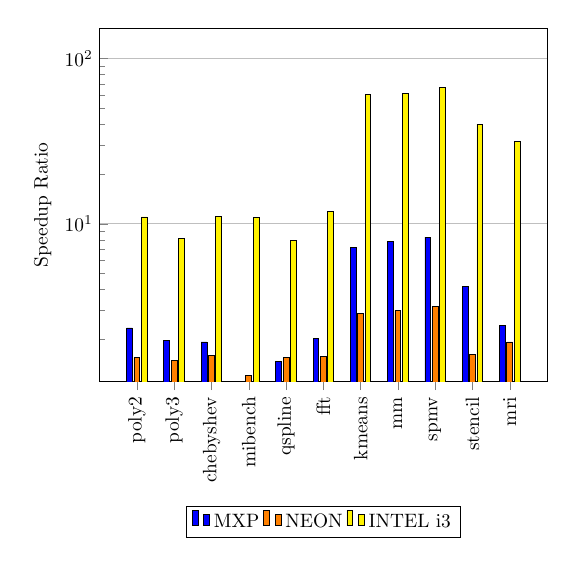
\begin{tikzpicture}[scale=0.7]
	\begin{semilogyaxis}[
	width  = 0.8*\textwidth,
	height = 8cm,
	xtick pos=left,
	ytick pos=left,
	%	major x tick style = transparent,
	x tick label style={rotate=90, anchor=east, align=right,text width=2cm},
	bar width=3pt,
	ymajorgrids = true,
	ylabel = {Speedup Ratio},
	symbolic x coords={poly2,poly3,chebyshev,mibench,qspline,fft,kmeans,mm,spmv,stencil,mri},
	xtick = data,
%	nodes near coords,
%	ybar,
%	every node near coord/.append style={rotate=90, anchor=west,font=\tiny},
	scaled y ticks = false,
	enlarge y limits={upper,value=0.2},
	%test
	%	enlarge x limits=0.25,
	ybar=2*\pgflinewidth,
	legend cell align=left,
	legend style={
		at={(.5,-0.35)},
		anchor=north,
		legend columns=-1
		column sep=0.5ex
	}
	]
	\addplot[draw=black,fill=blue]
	coordinates {(poly2,2.35) (poly3,1.98) (chebyshev,1.933) (mibench,1.11) (qspline,1.47) (fft,2.033) (kmeans,7.20) (mm,7.779) (spmv,8.32) (stencil,4.20) (mri,2.42) };
	
	\addplot[draw=black,fill=orange]
	coordinates	{(poly2,1.55 ) (poly3,1.49) (chebyshev,1.61) (mibench,1.22) (qspline,1.55) (fft,1.58) (kmeans,2.86) (mm,2.98) (spmv,3.16) (stencil,1.63) (mri,1.934) };
	
	\addplot[draw=black,fill=yellow]
	coordinates	{(poly2,11 ) (poly3,8.14) (chebyshev,11.13) (mibench,10.97) (qspline,7.95) (fft,11.85) (kmeans,60.42) (mm,61.53) (spmv,67.023) (stencil,40.039) (mri,31.28) };
	
	\legend{MXP,NEON,INTEL i3}
	\end{semilogyaxis}	
	\end{tikzpicture}
	\caption{Word level Speedup Analysis w.r.t ARMv7 for  different benchmarks.}
	\label{speedup:3}
\end{figure}

   
%    \begin{figure}
%    	\centering
%    	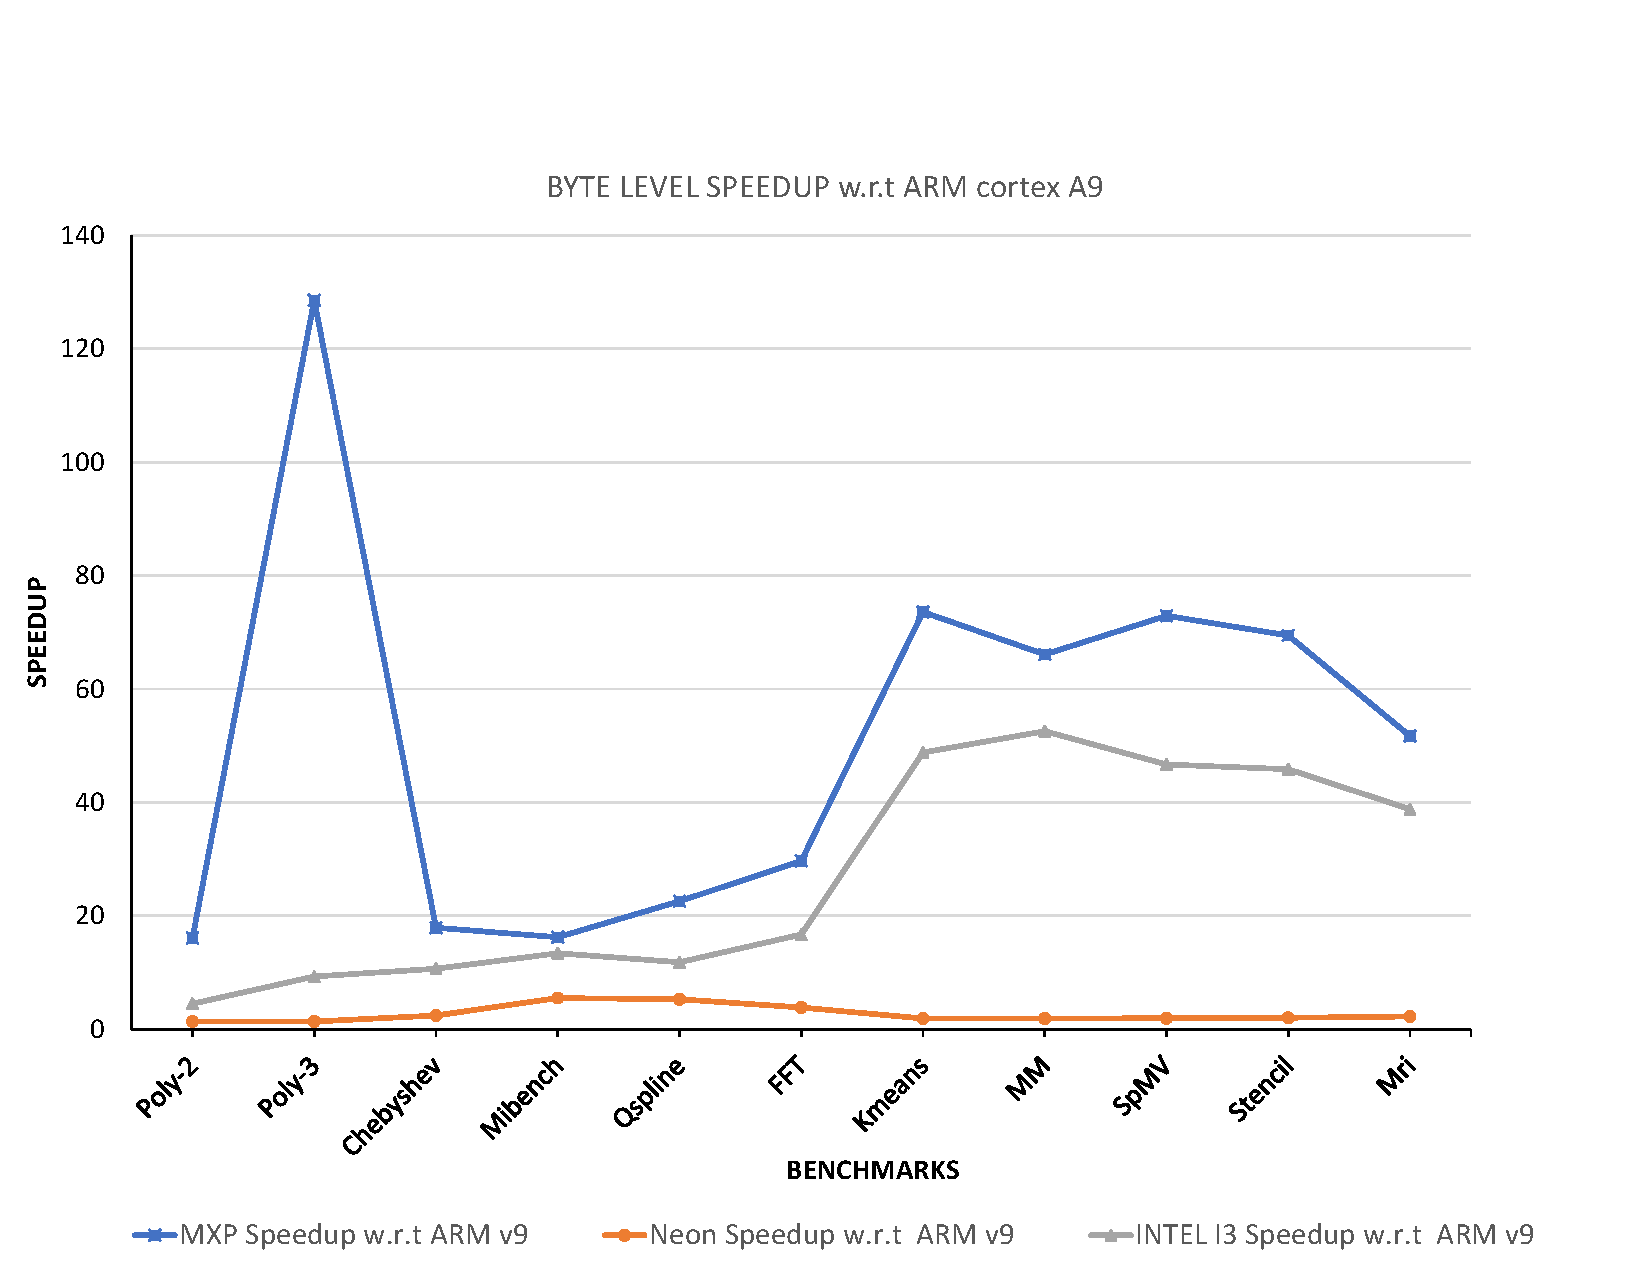
\includegraphics[width=.7\textwidth]{images/speedupbyte.pdf}
%    	\caption{Byte(8-bits) level Speedup w.r.t ARM A9}
%    	\label{random:1000}
%    \end{figure}
%  
% 
%    
%    \begin{figure}
%    	\centering
%    	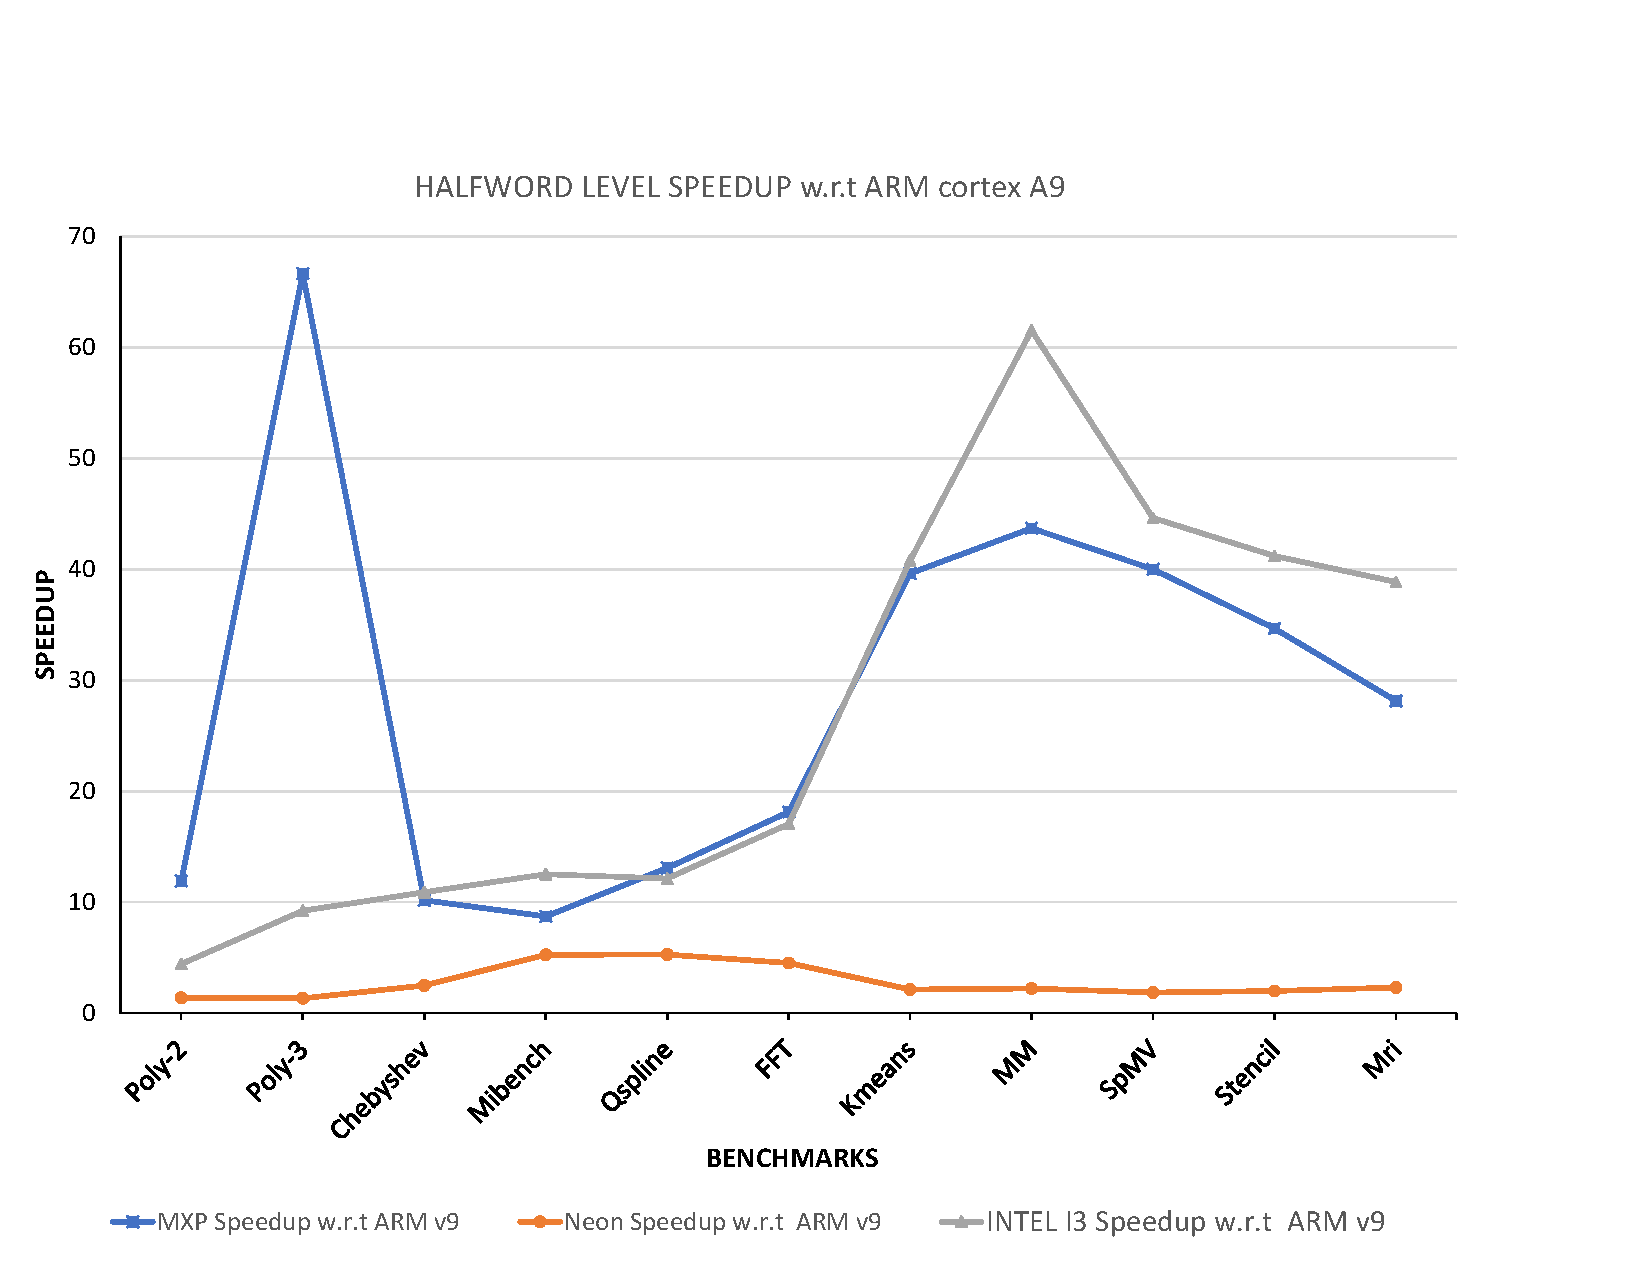
\includegraphics[width=.7\textwidth]{images/speeduphalf.pdf}
%    	\caption{Halfword(16-bits) level Speedup w.r.t ARM A9}
%    	\label{randomm:10000}
%    \end{figure}
%
%
%\begin{figure}
%	\centering
%	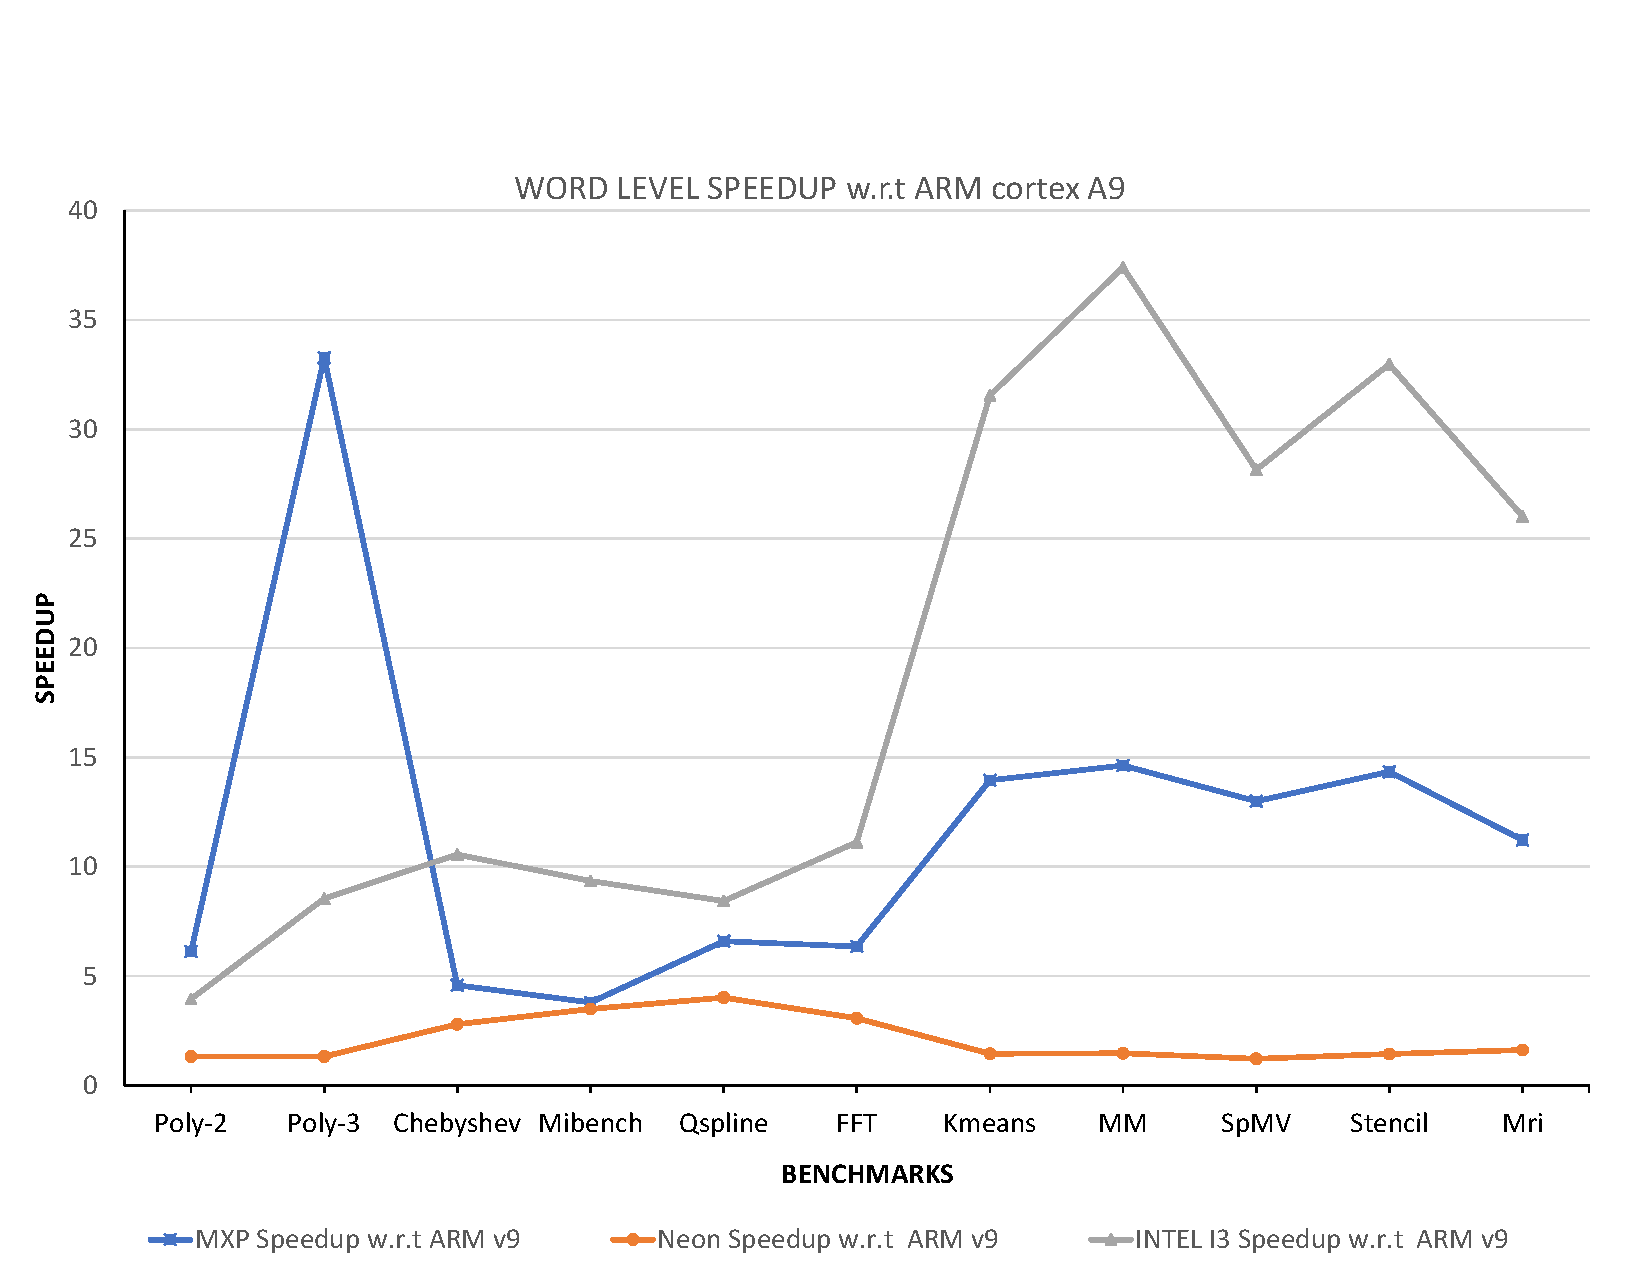
\includegraphics[width=.7\textwidth]{images/speedupword.pdf}
%	\caption{Word(32-bits) level Speedup w.r.t ARM A9}
%	\label{randommm:100000}
%\end{figure}
    
%    \section{Source Code for Measuring Performance}
    
%    The code for calculating the throughput for standard  kernels can be found in the below link:
    
%    Github Link : \url{https://github.com/AdhikariSaurabh/mxpbenchmarks}

%test
%
%\begin{figure}
%	\centering
%	\begin{tikzpicture}
%	\begin{axis}[
%	width  = 0.8*\textwidth,
%	height = 8cm,
%	%	major x tick style = transparent,
%	x tick label style={rotate=90, anchor=east, align=right,text width=2cm},
%	bar width=3pt,
%	ymajorgrids = true,
%	ylabel = {Throughput in $Gops/sec$},
%	symbolic x coords={poly2,poly3,chebyshev,mibench,qspline,fft,kmeans,mm,spmv,stencil,mri},
%	xtick = data,
%	nodes near coords,
%	ybar,
%	every node near coord/.append style={rotate=90, anchor=west,font=\scriptsize},
%	scaled y ticks = false,
%	enlarge y limits={upper,value=0.2},
%	%test
%	%	enlarge x limits=0.25,
%	ybar=2*\pgflinewidth,
%	legend cell align=left,
%	legend style={
%		at={(.5,-0.3)},
%		anchor=north,
%		legend columns=-1
%		column sep=0.5ex
%	}
%	]
%	\addplot[draw=black,fill=blue]
%	coordinates {(poly2, 0.1587) (poly3,0.2079) (chebyshev,0.142) (mibench,0.1279) (qspline,0.134) (fft,0.138) (kmeans,0.1279) (mm,0.134) (spmv,0.138) (stencil,0.134) (mri,0.138) };
%	
%	%	\addplot[draw=black,fill=orange]
%	%	coordinates  {(FFT, 0.278) (KMEANS,0.4702) (MM,0.3628) (SPMV,0.277) (STENCIL,0.308) (MRI,0.3201)};
%	
%	%	\addplot[draw=black,fill=yellow]
%	%	coordinates  {(FFT, 0.025) (KMEANS,0.0149) (MM,0.0097) (SPMV,0.00984) (STENCIL,0.00934) (MRI,0.0123)};
%	
%	%	\addplot[draw=black,fill=red]
%	%	coordinates {(FFT, 0.0769) (KMEANS,0.0216) (MM,0.01435) (SPMV,0.012) (STENCIL,0.0134) (MRI,0.02)};
%	\end{axis}	
%	\end{tikzpicture}
%	\caption{Comparing speedup in different benchmarks.}
%	\label{speedupcomparison}
%\end{figure}
%


\newpage
\chapter{Accelerating Image Processing and SpMV}

\section{Basic Image Processing Application}

We need to compile vbxapi library present in MXP repository to use MXP API’s, on Linux. Once built, this library needs to be linked while compiling the application which we will write on Linux. To start with, we built application for image negation and scaling operations. The input and processed image obtained after running the image negation application are shown in Figure~\ref{lena:7}

\begin{figure}
	\centering
	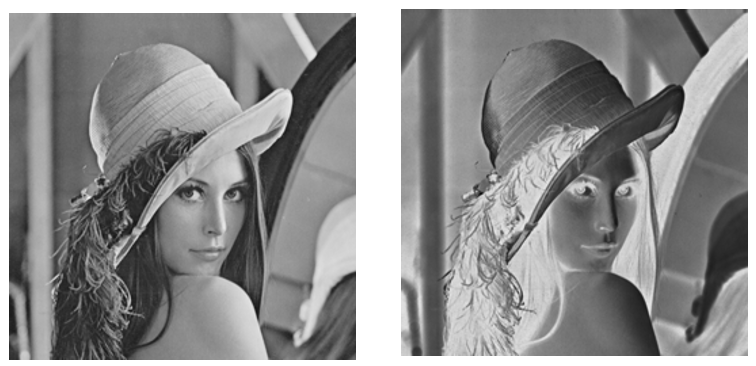
\includegraphics[width=.9\textwidth]{images/lena.png}
	\caption{Results of the Image Negation}
	\label{lena:7}
\end{figure}

The MXP application code for processing the input image for a negation operation is provided in Figure~\ref{cod:7}


%\lstinputlisting[firstline=89, lastline=132, frame=none,numbers=left,basicstyle=\fontsize{10}{10}\selectfont\ttfamily, backgroundcolor=\color{gainsboro}]{CodeSnippet.txt}


\begin{figure}
	\centering
	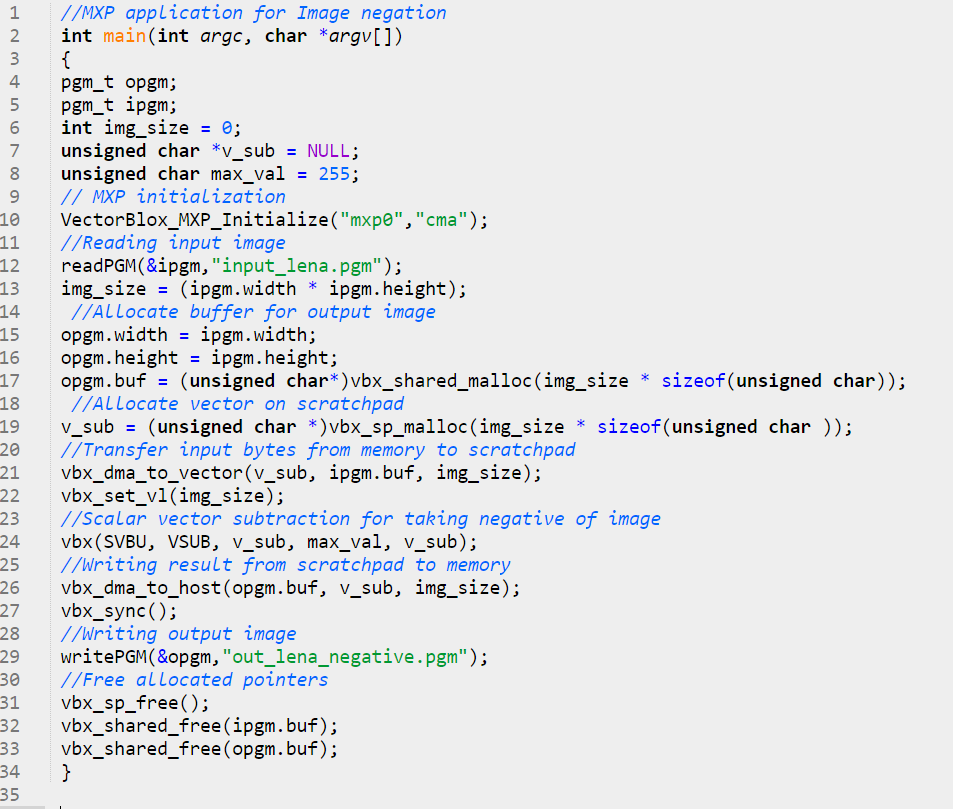
\includegraphics[width=1\textwidth]{images/code2.png}
	\caption{MXP application for Image negation}
	\label{cod:7}
\end{figure}


%\lstinputlisting[language=c,firstline=89, lastline=122, frame=none,numbers=left,basicstyle=\fontsize{11}{13}\selectfont\ttfamily, backgroundcolor=\color{gainsboro}]{hi.txt}

\section{Experiments and Results}

We took images of different dimensions and tried building image negative application for different platforms such as ARM v7, MXP and SIMD NEON unit. We tested the application with 128 X 128 pixels and 256 X 256 pixels. The runtime for the MXP soft-vector processor was then compared with the other processors. We observed that MXP seems to outperform other processors with a very good runtime obtained.  Table~\ref{ga:100} shows the runtime analysis of the MXP against the other processors.

\begin{table}[htbp]
	\centering
		\begin{adjustbox}{width=.9\textwidth}
		\small
	\begin{tabular}{lllll}
		\toprule
		\textbf{Metrics} & \textbf{ARMv7 CPU} & \textbf{NEON (auto vector)} & \textbf{MXP} \\
		\midrule
		\textbf{arch} & Scalar & SIMD unit & Vector \\
		\textbf{clock} & $667 x 10^{6}Hz$ & $667 x 10^{6}Hz$ & $110 x 10^{6}Hz$ \\
		\textbf{no of lanes} & 1 & 2 x 32b & 1-16 x 32b \\
		&   & 4 x 16b & 2-32 x 16b \\
		&   & 8 x 8b & 4-64 x 8b \\
		\midrule
	\textbf{Runtime (milliseconds)} &   &   &  \\
		\midrule
     128 x  128      pixels & 0.406 & 0.424 & 0.03686  \\	
	 256 x  256      pixels & 1.714 & 1.198 & 0.1843  \\
		\bottomrule
	\end{tabular}%
     \end{adjustbox}%
	\caption{Image Processing Runtime Analysis}
		\label{ga:100}%
\end{table}%



\section{Accelerating the SpMV Computational Kernel}

Sparse matrix dense vector also known as SpMV is one of the widely used computational kernel. It finds its application to solve the sparse linear system in information retrieval and many other applications. Since it is widely used, it is important to have a benchmark for SpMV. However, SpMV is really very difficult to benchmark because the data structure which is used in sparse matrix, it's density of the non-zero entries and it's dimensions - all have a significant impact on SpMV performance \cite{24},\cite{25}. We present a method on how the pre-existing benchmark for SpMV can be used and how MXP soft-processor can be used to accelerate the SpMV.

\subsection{SpMV basics}
	
In the case of a dense matrix, simple contiguous array is used as the data structure containing all the entries. Two orderings are most common: 
\begin{enumerate}

	\item row- major, where the rows are stored contiguously.
	\item column-major, where the columns are stored contiguously.
 
\end{enumerate}

The sparse multiplication depends on the structure of the sparse matrix. We can have regular and irregular structure for the SpMV. The general idea of performing a SpMV is to decompose the matrix into regular and the irregular parts. Compressed Sparse Row Format and Compressed Sparse Column Format are the basic formats in which the sparse matrix 
are stored.

\subsubsection{Compressed Sparse Row Format}

In CSR format, all the nonzero entries of the matrix will be in the form of row-major order consisting of two different arrays namely row\_start and col\_idx. The row\_start consist of index of non-zero entry present in the matrix in each row and the col\_index consist of the index of the non-zero entry present in the matrix in each column. Figure~\ref{aa:100} shows how the matrix elements will be stored while using the CSR format.

\begin{figure}
	\centering
	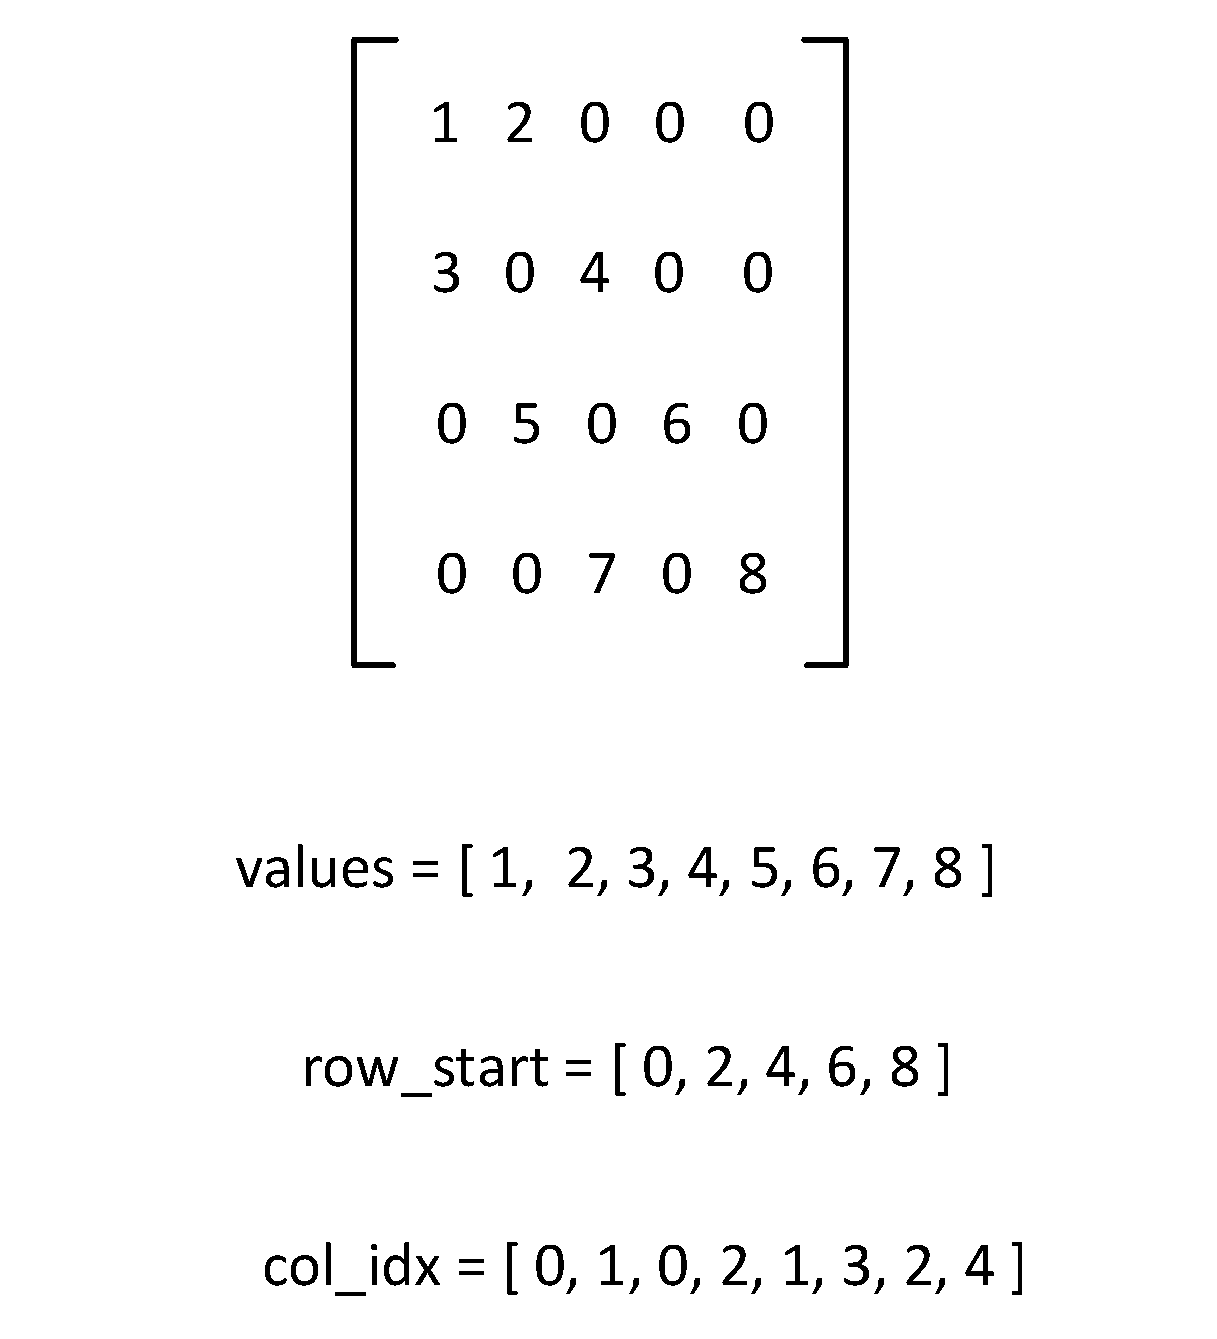
\includegraphics[width=.4\textwidth]{images/csr.pdf}
	\caption{Compressed Sparse Row Format}
	\label{aa:100}
\end{figure}

\subsubsection{Compressed Sparse Column Format}

In CSC format, all the nonzero entries of the matrix are kept in form of column major order consist-ing of two arrays namely col\_start and row\_idx. The col\_index consists of index of element of each row present and row\_idx consist of the index of the non-zero entry present in each row of matrix. The figure shows how the matrix elements will be stored while using the CSR format. When above Figure~\ref{aaa:1000} is stored in Compressed Sparse Row (CSR), it will be represented in the following form

\begin{figure}
	\centering
	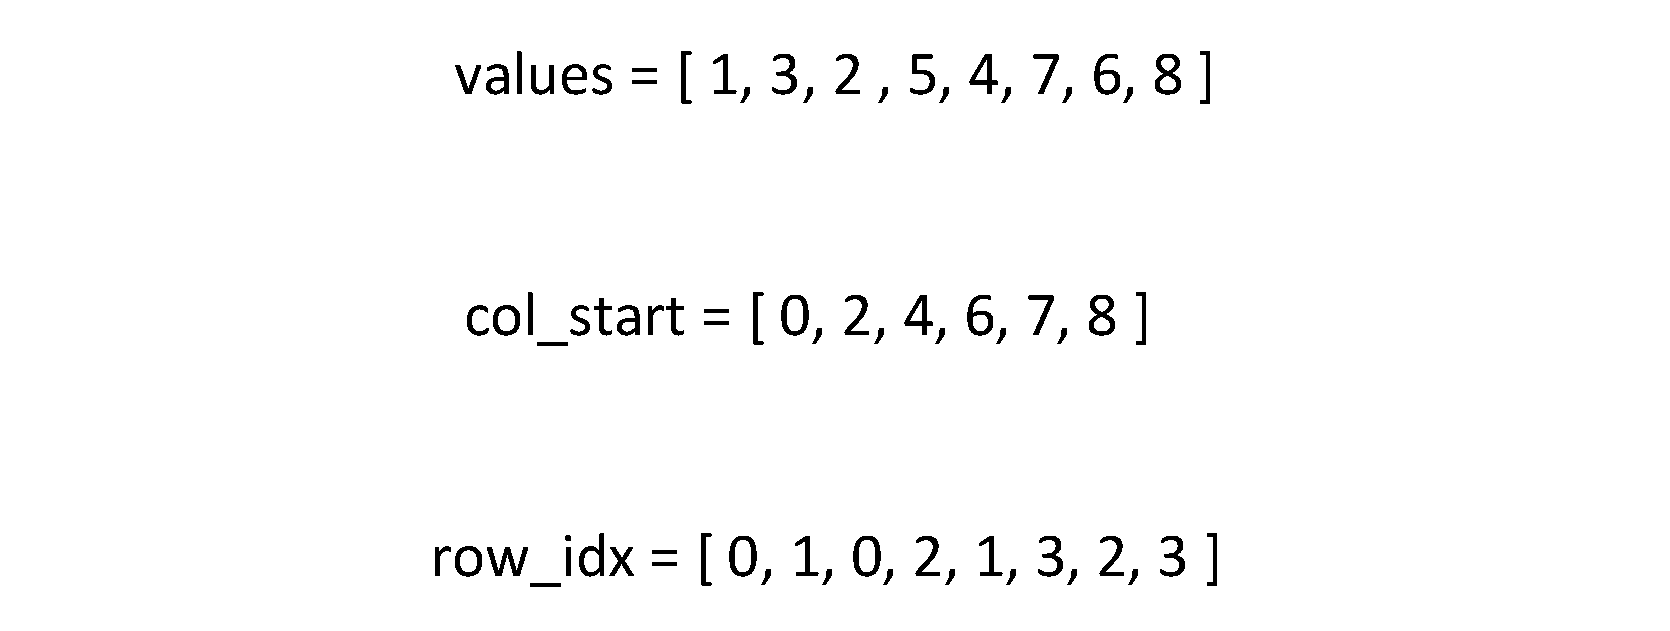
\includegraphics[width=.6\textwidth]{images/csc.pdf}
	\caption{Compressed Sparse Column Format}
	\label{aaa:1000}
\end{figure}

\subsection{Details of Pre-existing SpMV Benchmark}

The Pre-existing benchmarking framework mentioned in \cite{24}, stores the elements of the matrix in BCSR (Blocked Compressed Sparse Row) format. The idea behind the BCSR is to divide a given sparse matrix of size m x n into blocks of size r x c. By doing so we would obtain m / r blocks of rows and n / c blocks of columns which further can be stored in CSR format. Hence, at the end we will obtain m / r blocks where each of them represents r number of rows of the matrix and n / c blocks where each of them represents c number of columns of the matrix. This method helps in improving the accessing the elements of the sparse matrix and efficiently storing them in contiguous array either in row order or column order form. The operations are performed very efficiently providing high speedups. The blocks inside the dense matrix in Figure~\ref{aaaa:10000} are coloured and row major ordering is being used.  


\begin{figure}
	\centering
	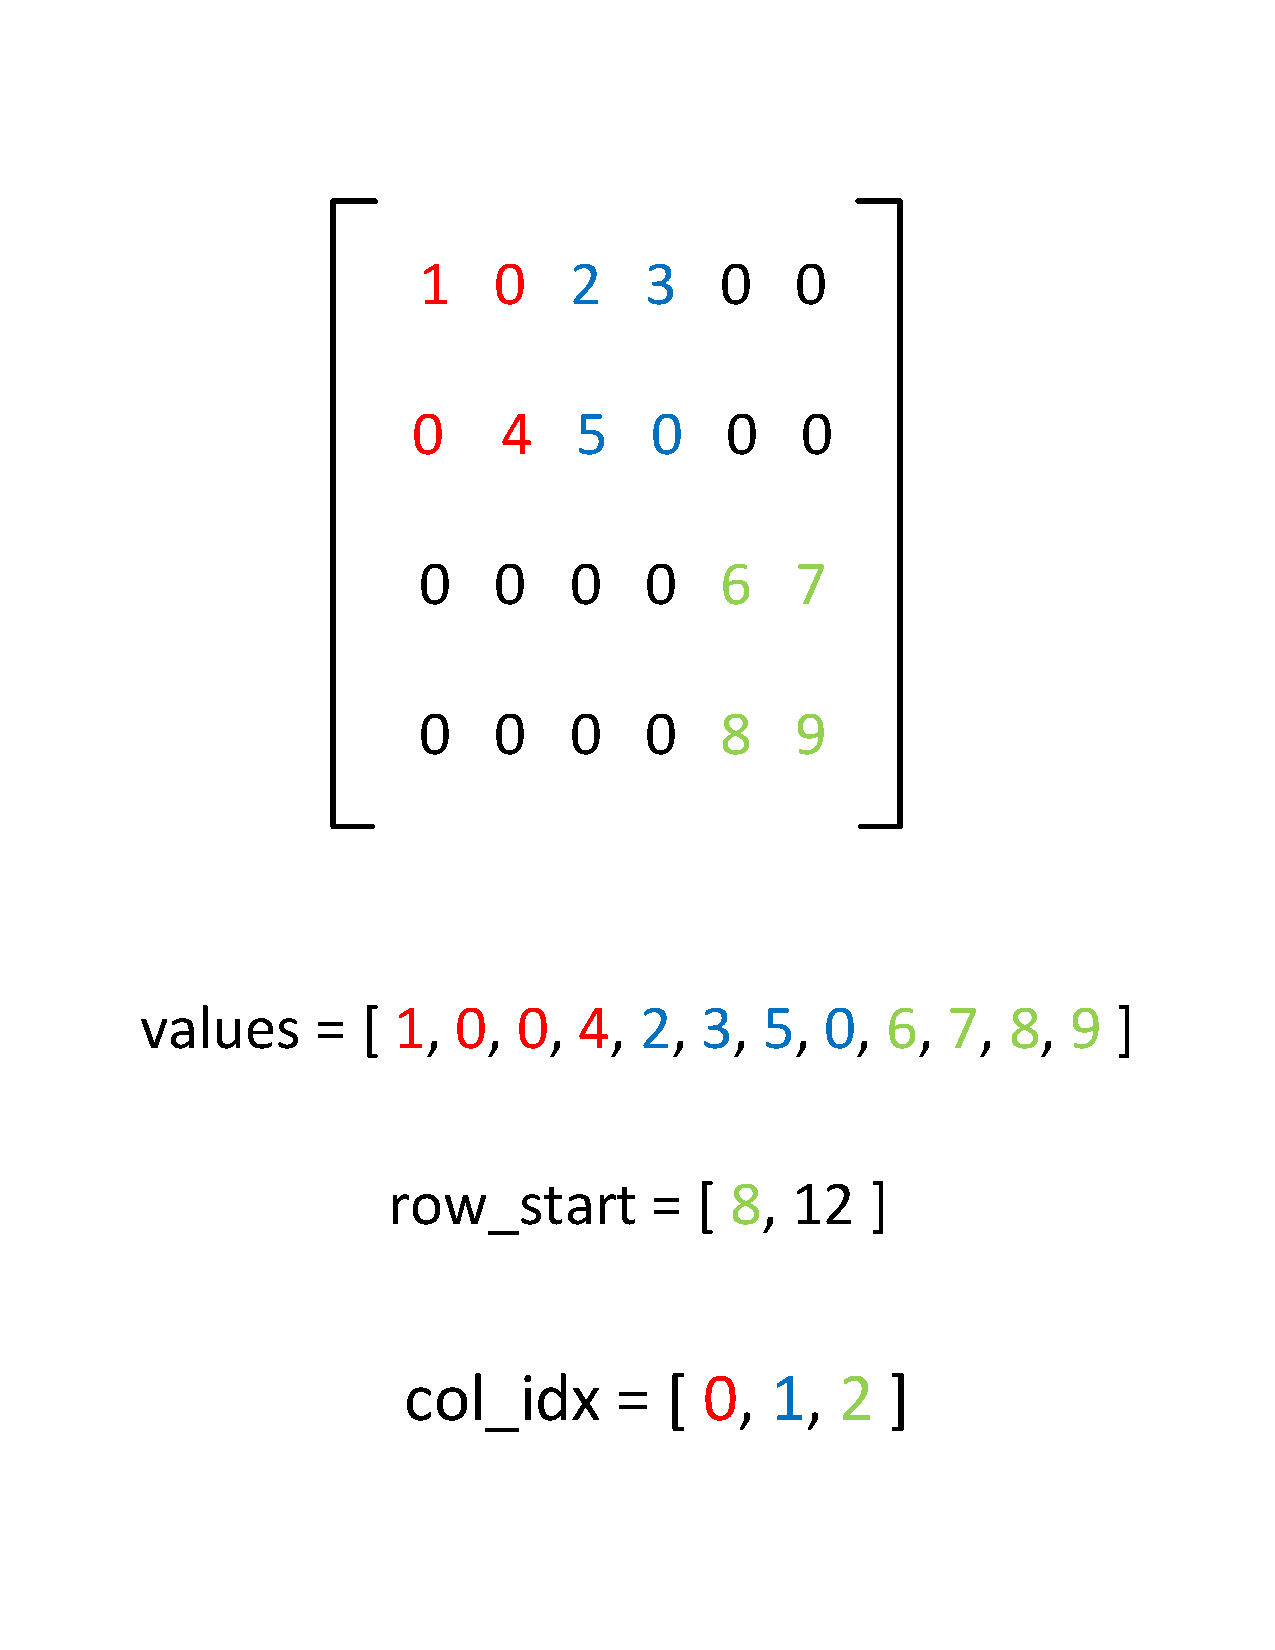
\includegraphics[width=.6\textwidth]{images/bcr.pdf}
	\caption{Blocked Compressed Sparse Row ordered}
	\label{aaaa:10000}
\end{figure}

\subsection{SpMV Usage Parameters}

When the main application will run in the existing framework it will generate the following usage parameters. User have the freedom to select one of the pre-defined block size. Below are the results which were obtained when Block Dim (r x c) was by default set to 1 x 1. Table~\ref{ww:101} shows the list of the SpMV usage parameters.
%\begin{figure}
%	\centering
%	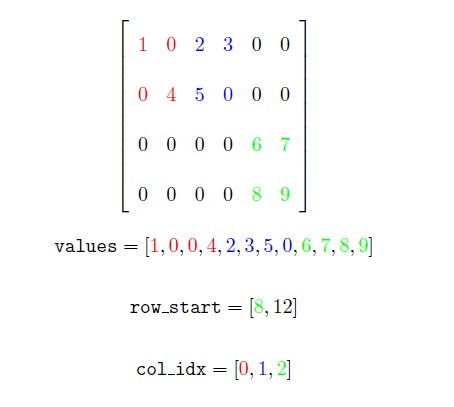
\includegraphics[width=.6\textwidth]{images/bcsr.jpg}
%	\caption{Blocked Compressed Sparse Row ordered}
%	\label{aaaa:10000}
%\end{figure}



\begin{table}[htbp]
	\centering	
	\begin{adjustbox}{width=.4\textwidth}
		\small
  \begin{tabular}{ll}
		\toprule
		\textbf{Parameters} & \textbf{Usage} \\
		\midrule
		   SpMV time & 0.886775 \\
		   Oper Time & 0.886774 \\
		   Cache time & 0.000001 \\
		   Matrix Dim (r x c) & 2097152 x 2097152 \\
		   Block Dim (r x c) & 1 x 1 \\
		   Non-zero blocks & 71303168 \\
		   Repetitions & 1 \\
		   Mflop/s & 160.814565 \\
		   num\_loads & 293601308 \\
		   num\_stores & 570425344 \\
		\bottomrule
	\end{tabular}%
\end{adjustbox}%
\caption{SpMV Usage}
\label{ww:101}%
\end{table}%

This pre-existing benchmarking framework consist of the block routine of dimensions \{2 x 2\}, \{4 x 4\}, \{8 x 8\}... Based on the block size we divide the sparse matrix into different blocks. This gives some hint to accelerate this benchmarking framework for SpMV by changing these block routines using the MXP APIs.


\subsection{Accelerating SpMV Framework Using MXP APIs}

MXP APIs are configured for the existing benchmarking framework so that we can use these APIs to accelerate the benchmarking process of the SpMV. There are block routines which are present in the existing framework. These block routines operate on the given sparse matrix at the block level. Thus, using the MXP APIs the block routines are modified to improve its performance.  Table~\ref{www:1010} shows the speedup obtained while performing SpMV multiplication which is in the form of $y = Ax$, one of the widely used computational kernel where A is a Sparse Matrix and x is the input vector and output y is the dense matrix. Result analysis shows that while performing SpMV product the MXP soft processor can be faster than ARMv7 ($2.07\times$).


\begin{table}[htbp]
	\centering
	
	\begin{adjustbox}{width=.7\textwidth}
		\small
		
	\begin{tabular}{lllll}
		\toprule
		\textbf{Metrics} & \textbf{ARMv7 CPU} & \textbf{MXP}  \\
		\midrule
		\textbf{uarch} & Scalar & Vector \\
		\textbf{Clock} & $667 X 10^{6} Hz$ & $110 X 10^{6}Hz$  \\
		\textbf{No of Lanes} & 1 & 1-16 x 32b  \\
		&   & 2-32 X16b  \\
		&   & 4-64 X8b \\
		&   &   \\
		\midrule
		\textbf{Runtime (millisecond)  } &   &   &   &  \\
		\midrule
		\textbf{SpMV \{25 x 25\} kernel} & 0.037 & 0.01843  \\
		\textbf{SpMV \{50 x 25\} kernel} & 0.055 & 0.03686  \\
		\bottomrule
	\end{tabular}%
    \end{adjustbox}%
      \caption{Runtime for SpMV kernel Computation}
	\label{www:1010}%
\end{table}%	
    	 

\section{SpMV Kernel Code}

The algorithm along with the code for calculating the runtime for SpMV kernel Computation can be found in the below link:

Github Link : \url{https://github.com/AdhikariSaurabh/mxpbenchmarks/tree/master/SpMV}







\newpage
\chapter{Conclusion and Future Work}

\section{Conclusions}

This thesis focuses upon using FPGA overlay architecture as an accelerator for accelerating different standard benchmarks. Configuring the Linux for MXP on the ZedBoard to provide the OS support for MXP is among one of the work done in this thesis. The performance, speedup and runtime analysis of different compute kernels are obtained using the MXP overlay as a FPGA accelerator. Moreover, MXP performance is compared with different embedded hard processors such as ARM v7, NEON SIMD unit and INTEL i3. The performance in terms of throughput was measured at the byte, halfword and word level.

We accelerated Poly-2 and Poly-3 benchmarks where we could get a very high throughput as well as speedup using the MXP overlay. The results show that MXP provides speedup of ${\approx}4.5$ times the speedup provided by ARM v7 and speedup of ${\approx}1.5$ times the speedup provided by NEON SIMD unit. Throughput obtained by the MXP while accelerating poly benchmarks was 1.5130 (Gops/sec) for poly-2 and 2.287 (Gops/sec) for poly-3 benchmark which is higher as compared to throughput obtained by other processors. The above results are mentioned for the word (32-bits) level operation whereas this thesis covers the throughput measurement at byte (8-bits) and halfword (16-bits) level also.

Filter kernels such as CHEBYSHEV, QSPLINE and MIBENCH were accelerated using MXP. For CHEBYSHEV, we could get throughput of 1.41 (Gops/sec) which is greater than SIMD NEON unit and ARM v7 processor. For MIBENCH, we could get throughput of 1.54 (Gops/sec) which is greater than SIMD NEON unit and ARM v7 processor. For QSPLINE, we could get throughput of 1.76 (Gops/sec) which is greater than SIMD NEON unit and ARM v7 processor. The above results are mentioned for the word (32-bits) level operation whereas this thesis covers the throughput measurement at byte (8-bits) and halfword (16-bits) level also.


Standard kernels such as FFT, KMEANS, MM, SPMV, STENCIL and MRI were also accelerated using MXP. For FFT, we could get throughput of 0.699 (Gops/sec) which is greater than SIMD NEON unit and ARM v7 processor. For KMEANS, we could get throughput of 0.9143 (Gops/sec) which is greater than SIMD NEON unit and ARM v7 processor. For MM, we could get throughput of 0.62 (Gops/sec) which is greater than SIMD NEON unit and ARM v7 processor. For SPMV, we could get throughput of 0.55 (Gops/sec) which is greater than SIMD NEON unit and ARM v7 processor. For STENCIL, we could get throughput of 0.589 (Gops/sec) which is greater than SIMD NEON unit and ARM v7 processor. For MRI, we could get throughput of 0.388 (Gops/sec) which is greater than SIMD NEON unit and ARM v7 processor. The above results are mentioned for the word (32-bits) level operation whereas this thesis covers the throughput measurement at byte (8-bits) and halfword (16-bits) level also.



Polybench kernels, ATAX and BiCG were accelerated using MXP. For ATAX, we could get speedup of ${\approx}6$ for small dataset size and ${\approx}5$ for standard dataset size. For BiCG, we could get speedup of ${\approx}7$ for small dataset size and ${\approx}3$ for standard dataset size.



We also accelerated an image processing application using the MXP overlay and measured the runtime. The time took by the MXP was 0.03686 milliseconds for image having dimension as 128 X 128 pixels and 0.1843 milliseconds for image having dimension as 256 X 256 pixels. The speedup provided by the MXP overlay was very high when compared with the speedup provided by ARM v7, NEON SIMD unit and INTEL i3 processors. SpMV existing benchmarking framework was configured such that MXP APIs can be used to accelerate SpMV computational kernel.



\section{Future Work}

\subsection{Power Analysis}
In our work, focus was more on throughput (Gops/sec) as one of the performance parameter. We can run different MXP applications and measure the power dissipated. The power rails of the ZedBoard gives some hints of measuring the power for the application running on the ZedBoard. 

\subsection{Audio Processing Application}
Building an audio processing application and accelerating it using the MXP overlay. The performance analysis for the audio processing application and its comparison with the other embedded hard processors like ARM v7, SIMD NEON unit and INTEL i3.

\subsection{Completion of the SpMV Benchmarking Framework}
The current existing SpMV benchmarking framework consist of different block routines that divide the input sparse dense matrix into different blocks and then process it i.e. BCSR (Blocked Compressed Sparse Row). The MXP APIs can be used to build and change the entire block routines to accelerate the SpMV computational kernel.  



\begin{thebibliography}{1}
%\addcontentsline{toc}{chapter}{References}

\bibitem{kapre2016optimizing}Nachiket Kapre, \emph{Optimizing Soft Vector Processing in FPGA-based Embedded
	Systems}, \url{http://nachiket.github.io/publications/soft-vector_trets2016.pdf}

\bibitem{1}Charles Eric LaForest, \emph{High Speed Soft Processor Architecture for FPGA Overlays}, \url{http://fpgacpu.ca/octavo/High-Speed_Soft-Processor_Architecture_for_FPGA_Overlays.pdf}

\bibitem{2}Overlay Architectures for FPGA (OLAF), Berkeley. \url{http://olaf.eecs.berkeley.edu}

\bibitem{3}Michael Feldman and Addison Snell, \emph{ACCELERATED COMPUTING: A TIPPING POINT FOR HPC.}
\url{http://images.nvidia.com/content/pdf/tesla/accelerated-computing-at-a-tipping-point.pdf}

\bibitem{4}Davor Capalija and Tarek S. Abdelrahman,\emph{FPGA Overlays for High Performance Computing.} \url{https://www.eee.hku.hk/~hso/olaf2013/abdelrahman_olaf.pdf}

\bibitem{5}Kevin Morris, \emph{FPGA Wars: It’s Getting Hot at the Top.}
\url{http://www.eejournal.com/archives/articles/20130305-fpgawars}

\bibitem{6}A. K. Jain, K. D. Pham, J. Cui, S. A. Fahmy, and D. L. Maskell,\emph{Virtualized
	execution and management of hardware tasks on a hybrid ARM-FPGA platform}, 2Journal of Signal Processing Systems, 77(1–2):61–76, Oct. 2014

\bibitem{7}Jesse Benson, Ryan Cofell, Chris Frericks, Chen-Han Ho, Venkatraman Govin-
daraju, Tony Nowatzki, and Karthikeyan Sankaralingam,\emph{Design, integration
	and implementation of the dyser hardware accelerator into opensparc}, In In-
ternational Symposium on High Performance Computer Architecture (HPCA),
pages 1–12, 2012

\bibitem{8}Neil W. Bergmann, Sunil K. Shukla, and Jrgen Becker,\emph{QUKU: a dual-layer
	reconfigurable architecture}, ACM Transactions on Embedded Computing Systems
(TECS), 12:63:1–63:26, March 2013

\bibitem{9}A. Severance and G. G. F. Lemieux,\emph{Embedded supercomputing in fpgas with the
	vectorblox mxp matrix processor}, In Hardware/Software Codesign and System
Synthesis (CODES+ISSS), 2013 International Conference on, pages 1–10, 2013

\bibitem{10}Xilinx Ltd. Zynq-7000 technical reference manual\url{http://www.xilinx.com/
	support/documentation/user_guides/ug585-Zynq-7000-TRM.pdf} 2013

\bibitem{11}\url{http://www.nxp.com/assets/documents/data/en/application-notes/AN4991.pdf}

\bibitem{12}\url{http://zedboard.org/sites/default/files/documentations/ZedBoard_HW_UG_v2_2.pdf}

\bibitem{13}Xilinx Ltd. Zynq-7000 technical reference manual\url{http://www.xilinx.com/
	support/documentation/user_guides/ug585-Zynq-7000-TRM.pdf}

\bibitem{14}Gordon Brebner,\emph{A virtual hardware operating system for the Xilinx XC6200}, In
Field-Programmable Logic Smart Applications, New Paradigms and Compilers,
pages 327–336. 1996

\bibitem{15}C. Steiger, H. Walder, and M. Platzner,\emph{Operating systems for reconfigurable
	embedded platforms: online scheduling of real-time tasks}, IIEEE Transactions
on Computers, 53(11):1393–1407, November 2004

\bibitem{16}C. Aws Ismail,\emph{Operating system abstractions of hardware accelerators on field-
	programmable gate arrays}, Thesis, August 2011

\bibitem{17}Xillybus Ltd. Xillybus: IP Core Product Brief\url{http://xillybus.com/downloads/xillybus_product_brief.pdf}

\bibitem{18}\url{http://www.wiki.xilinx.com/Linux}

\bibitem{19}\url{http://vectorblox.github.io/mxp/mxp_quickstart_vivado.html}

\bibitem{20}\url{http://vectorblox.github.io/mxp/mxp_reference.html}

\bibitem{21}S. Gopalakrishnan, P. Kalla, M. B. Meredith, and F. Enescu,\emph{Finding
	linear building-blocks for RTL synthesis of polynomial datapaths with
	fixed-size bit-vectors}, ICCAD, 2007

\bibitem{22}Abhishek Kumar Jain, Douglas L. Maskell,Suhaib A. Fahmy, \emph{Throughput Oriented FPGA Overlays Using DSP Blocks.}
\url{https://www2.warwick.ac.uk/fac/sci/eng/staff/saf/publications/date2016-jain.pdf}

\bibitem{23}Soh Jun Jie and N. Kapre,\emph{Comparing soft and hard vector processing in FPGA-based embedded systems}, 2014 24th International Conference on Field Programmable Logic and Applications (FPL), Munich, 2014, pp. 1-7.
doi: 10.1109/FPL.2014.6927467

\bibitem{24}Nachiket Kapre,\emph{Optimizing Soft Vector Processing in FPGA-Based Embedded Systems}, ACM Transactions on Reconfigurable Technology and Systems, vol. 9, pp. 1, 2016, ISSN 19367406

\bibitem{25}Hormozd Benjamin Gahvari, \emph{Benchmarking Sparse Matrix-Vector Multiply.}
\url{https://pdfs.semanticscholar.org/8abd/d65f91a25d724b393f5ff07cdd3f4b033468.pdf}

\bibitem{26}Rajesh Nishtala, Richard W. Vuduc, James W. Demmel, Katherine A. Yelick, \emph{Performance Modeling and Analysis of Cache Blocking in Sparse Matrix Vector Multiply.
}
\url{https://www2.eecs.berkeley.edu/Pubs/TechRpts/2004/CSD-04-1335.pdf}



\end{thebibliography}



\end{document}
